\documentclass[mathserif,serif]{beamer}
\useoutertheme{infolines}
%\usepackage{tabularx}
%\usepackage{amsmath}
\graphicspath{{data/plot/plot_SR/}}

\title[Lo Cheuk Yee]{Search for chargino and neutralino production in final states with two same-sign leptons, jets and missing transverse momentum at $\sqrt{s} = 13$ TeV with the ATLAS detector}
\author[]
{
Samuel Lo
}
\institute[]
{
The University of Hong Kong
}
\date[]{\today}

\newcommand\Wider[2][2em]{%
\makebox[\linewidth][c]{%
\begin{minipage}{\dimexpr\textwidth+#1\relax}
\raggedright
\centering#2
\end{minipage}%
}%
}

\begin{document}

\frame{\titlepage}
%\frame{\tableofcontents}

\begin{frame}{Contents}
\begin{itemize}
\item Introduction
\item Experimental Setup
\item Background
\begin{itemize}
\item Charge Flip Background
\item Fake Lepton Background
\end{itemize}
\item Signal Region
\item Validation Region
\item Results
\end{itemize}
\end{frame}

\section{Introduction}
\begin{frame}
\begin{center}
\huge
Introduction
\end{center}
\end{frame}

\begin{frame}{Standard Model : Fundamental Particles}
\begin{itemize}
\item Standard Model(SM) is the current mainstream theory to describe the electromagnetic force, weak force and strong force.
\end{itemize}

\begin{figure}
\centering
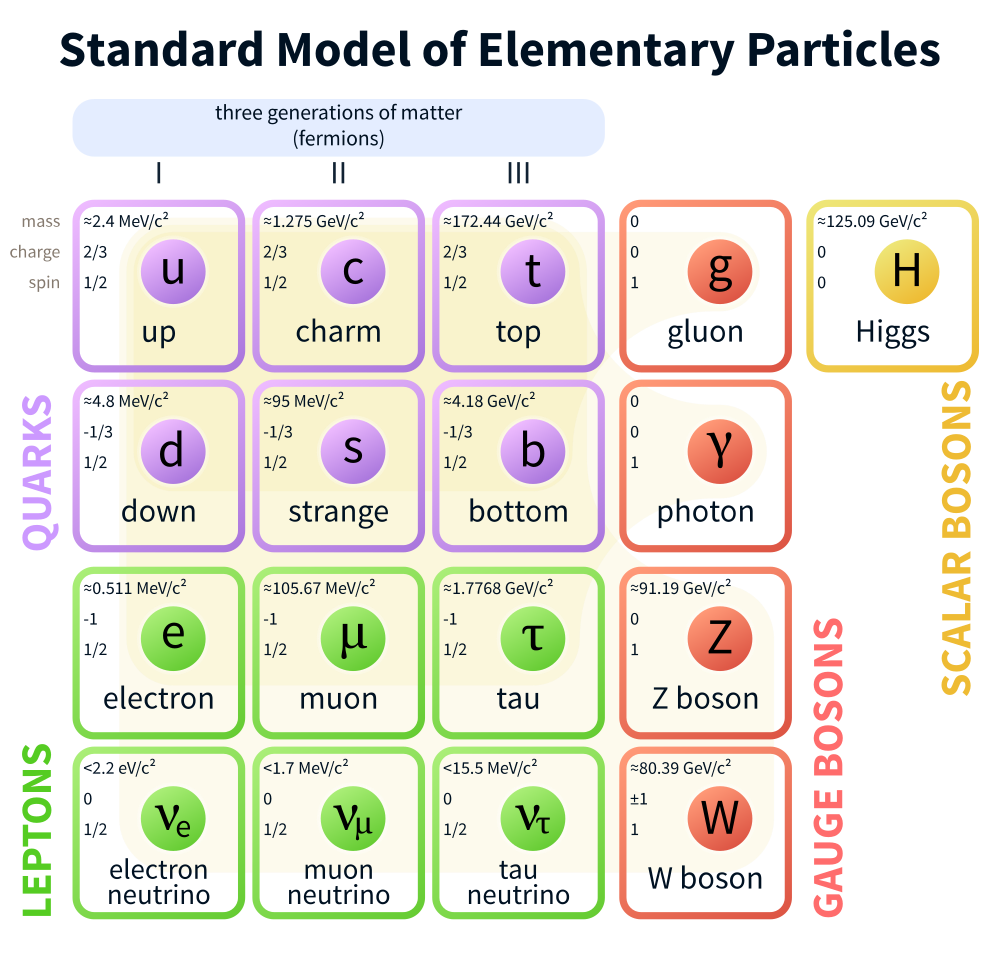
\includegraphics[width=0.5\textwidth]{data/photo/theory/SM_particles.png}
\caption{The ``periodic'' table for all fundamental particles in SM.}
\end{figure}
\end{frame}

\begin{frame}{Standard Model : Fundamental Interaction}
\begin{columns}

\begin{column}{0.5\textwidth}
\begin{figure}
\centering
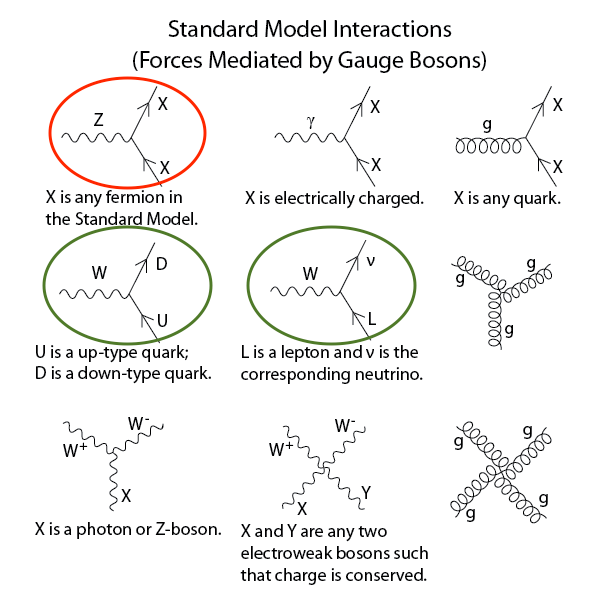
\includegraphics[width=\textwidth]{data/photo/theory/vertices_SM_circle.png}
\caption{All allowed fundamental Feynman vertices in SM, except higgs-related vertices.}
\end{figure}

\end{column}

\begin{column}{0.5\textwidth}
\begin{figure}
\centering
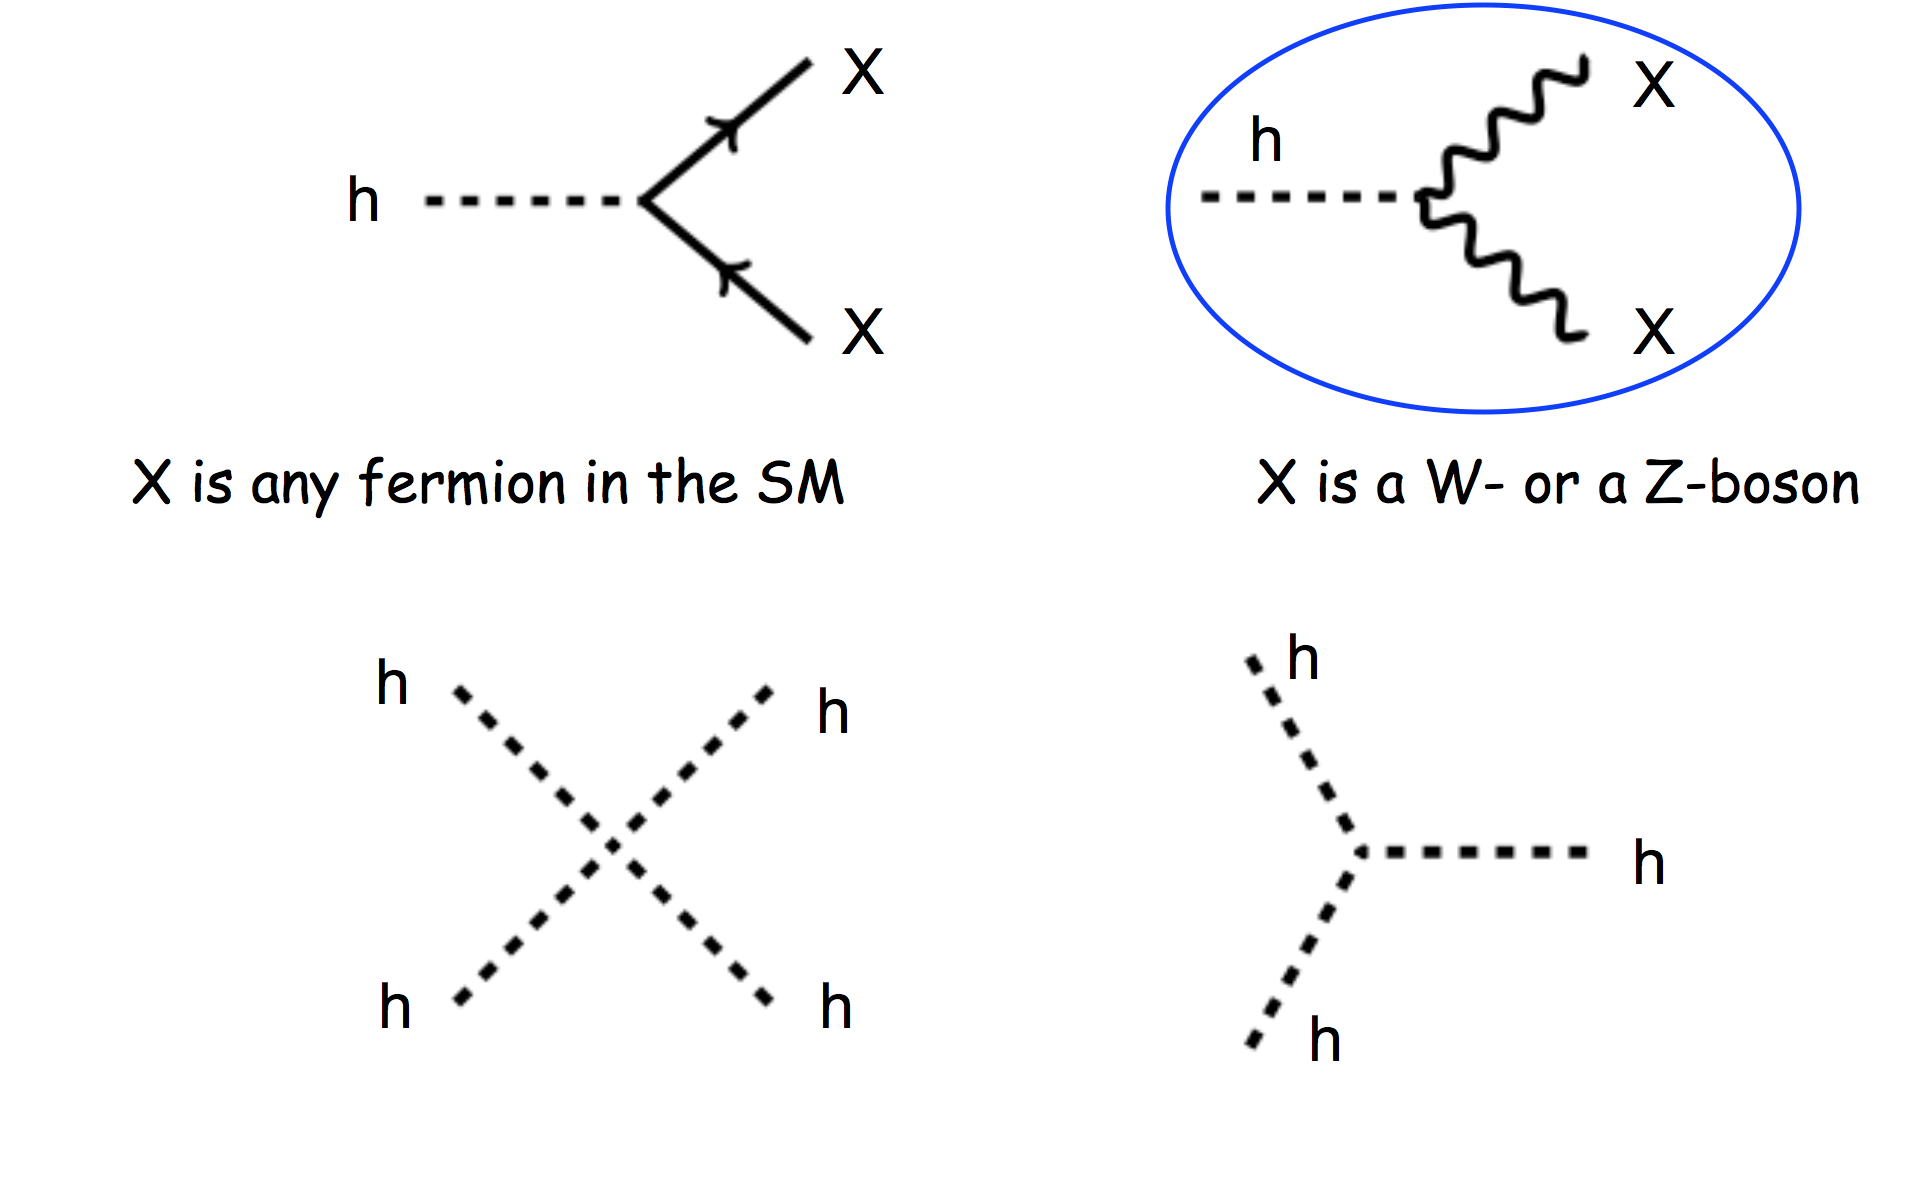
\includegraphics[width=\textwidth]{data/photo/theory/vertices_higgs_circle.png}
\caption{All allowed fundamental higgs-related Feynman vertices in SM.}
\end{figure}
\end{column}

\end{columns}
\end{frame}

\begin{frame}{Standard Model : Success}
SM gained a huge success in predicting experimental results.
\begin{itemize}
\item With the W boson explaining the beta decay, the existence of the neutral Z boson was predicted and discovered later in 1980s.
\item The existence of a third generation of quarks was predicted in 1970s and top quark was discovered in 1990s.
\item Higgs boson was proposed in 1960s and discovered recently in 2012.
\end{itemize}
\end{frame}

\begin{frame}{Standard Model : Limitation}
\begin{itemize}
\item SM cannot explain the nature of dark matter.
\item The hierarchy problem
\begin{itemize}
\item Why the weak force is stronger than the gravity by $10^{24}$.
\item The Higgs boson mass is quadratically divergent due to the quantum corrections.
\end{itemize}
\item The electroweak interaction and the strong interaction cannot be unified in SM.
\end{itemize}
\end{frame}

\begin{frame}{Supersymmetry}
\begin{itemize}
\item Supersymmetry is one of the most promising theory.
\item Supersymmetry(SUSY) is a theoretical extension of the Standard Model.
\item It can solve the hierarchy problem of Higgs mass.
\item It can explain the nature of dark matter.
\item It unifies the electroweak interaction and the strong interaction at $\sim 10^{16}$ GeV. The gauge couplings change with the energy scale.
\end{itemize}
\begin{figure}
\centering
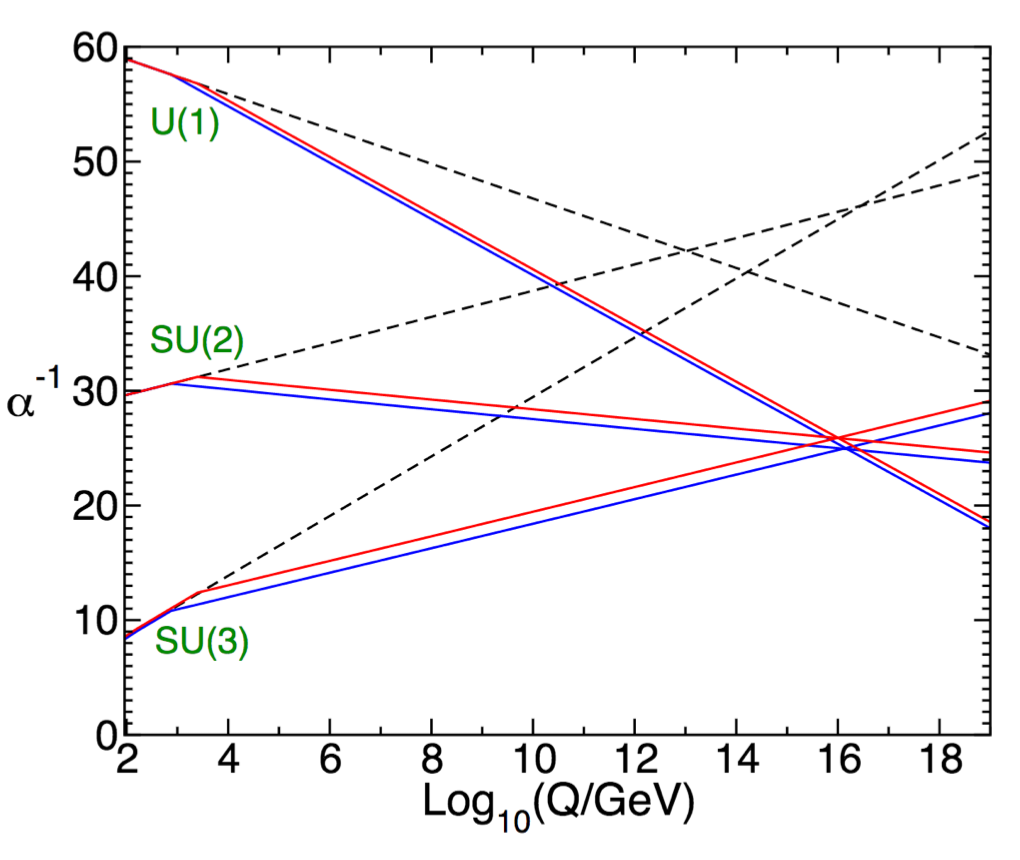
\includegraphics[width=0.3\textwidth]{data/photo/theory/unification.png}
\caption{Black dashed lines are for SM. Red and blue lines are for SUSY.}
\end{figure}
\end{frame}

\begin{frame}{Supersymmetry}
\begin{itemize}
\item It predicts that each particle in the Standard Model has its own partner particle, called the superpartner (SUSY particle).
\item The spin of the superpartner will differ from the Standard Model particle by 1/2.
\item A symmetry between the fermions and bosons.
\end{itemize}
\begin{figure}
\centering
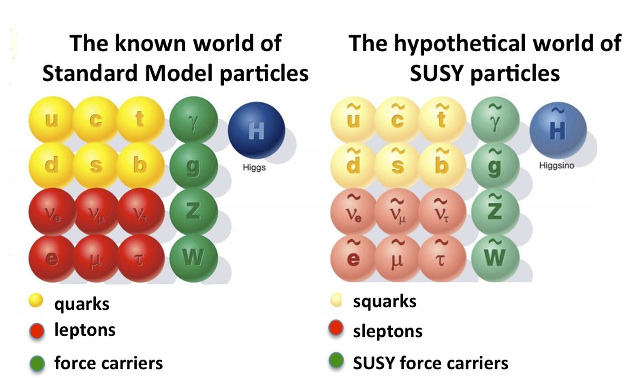
\includegraphics[width=0.4\textwidth]{data/photo/theory/SM-SUSY-diagram.jpg}
\caption{The particles in Standard Model and their corresponding superpartners and their names.}
\end{figure}
\end{frame}

\begin{frame}{Supersymmetry : Superpartners}
\begin{itemize}
\item In the simple SUSY models, we need two neutral Higgs fields ($H^0_u$ and $H^0_d$) and two charged Higgs fields ($H^+_u$ and $H^-_d$).
\item The superpartners of 4 neutral bosons $\gamma$, $Z$, $H^0_u$ and $H^0_d$ together form 4 mass eigenstates, called neutralinos: $\tilde{\chi}_1^0$, $\tilde{\chi}_2^0$, $\tilde{\chi}_3^0$ and $\tilde{\chi}_4^0$.
\item The superpartners of 4 charged bosons $W^+$, $W^-$, $H^+_u$ and $H^-_d$ together form two mass eigenstates with electric charge $\pm 1$, called charginos: $\tilde{\chi}_1^\pm$ and $\tilde{\chi}_2^\pm$.
\end{itemize}

\begin{table}[htbp]
\tiny
\centering
\scalebox{0.8}{
\begin{tabular}{|c|cccc|cccc|}
\hline
\hline
Type & SM particle & Symbol & Spin & R-parity & Superpartner & Symbol & Spin & R-parity \\
\hline
\hline
Fermions & Quark  & $q$ & $\frac{1}{2}$ & +1 & Squark  & $\tilde{q}$ & 0 & -1 \\
& Lepton & $l$ & $\frac{1}{2}$ & +1 & Slepton & $\tilde{l}$ & 0 & -1 \\
\hline
Gluon & Gluon  & $g$ & $1$ & +1 & Gluino & $\tilde{g}$ & $\frac{1}{2}$ & -1  \\
\hline
Neutral EW Bosons & Photon         & $\gamma$ & $1$ & +1
&  &  &  &  \\
& Z Boson        & $Z$      & $1$ & +1
& Neutralinos & $\tilde{\chi}_1^0$, $\tilde{\chi}_2^0$, $\tilde{\chi}_3^0$, $\tilde{\chi}_4^0$ & $\frac{1}{2}$ & -1 \\
& Neutral Higgs  & $H^0_u$, $H^0_d$  & $0$ & +1
&  &  &  &  \\
\hline
Charged EW Bosons & W Boson        & $W^+$, $W^-$  & $1$ & +1
& Charginos & $\tilde{\chi}_1^\pm$, $\tilde{\chi}_2^\pm$ & $\frac{1}{2}$ & -1 \\
& Charged Higgs  & $H^+_u$, $H^-_d$  & $0$ & +1
&  &  &  &  \\
\hline
\hline
\end{tabular}
}
\caption{\scriptsize The spin and R-parity for the Standard Model particles and their superpartners.}
\end{table}

\end{frame}

\begin{frame}{Supersymmetry : R-parity}
\begin{itemize}
\item In order to avoid the proton decay, a quantum number R-parity is introduced. All SM particles have R-parity $+1$, while all SUSY particles have R-parity $-1$.
\item If the R-parity is conserved, the lightest SUSY particle (LSP) cannot decay (stable).
\item If the LSP is electrically neutral and interacts with matter only by the weak interaction and gravity, it could be a candidate for dark matter, for example the lightest neutralinos $\tilde{\chi}_1^0$.
\item In this thesis, the R-parity is assumed to be conserved, and the lightest neutralino $\tilde{\chi}_1^0$ is assumed to be the LSP.
\item Due to the conservation of R-parity, the SUSY particles can only be pair-produced, and will eventually decay into SM particles and the lightest neutralino $\tilde{\chi}_1^0$ (i.e. LSP).
\end{itemize}
\end{frame}

\begin{frame}{Our Signal Scenario : Motivation}
\begin{itemize}
\item In the recent searches for SUSY particles involved in strong interaction, their masses are suggested to be larger than 1 TeV.
\item In this case, the direct pair production of SUSY electroweak boson $\tilde{\chi}_1^\pm$  and $\tilde{\chi}_2^0$ may be the dominant SUSY production process at the LHC, if their masses are below 1 TeV.
\item In this thesis, their masses are assumed to be the same, and denoted by $m_{\tilde{\chi}_1^\pm , \tilde{\chi}_2^0}$ (in simplified models).
\end{itemize}
\begin{figure}
\centering
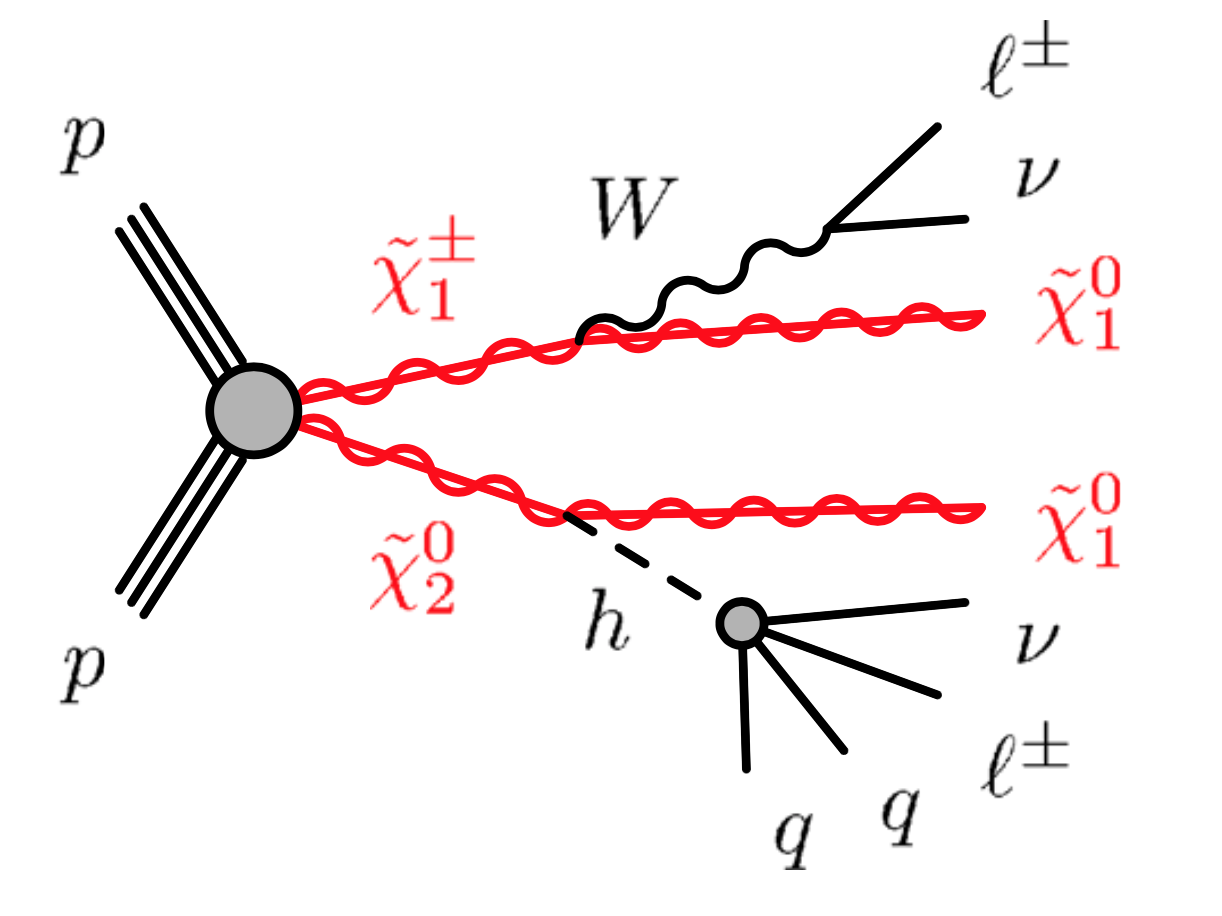
\includegraphics[width=0.3\textwidth]{data/photo/theory/signal_feynman.png}
\end{figure}
\end{frame}

\begin{frame}{Our Signal Scenario : Decay Processes}
\begin{itemize}
\item If all the slepton ($\tilde{l}$) are heavier than $\tilde{\chi}_1^\pm$ and $\tilde{\chi}_2^0$ :
\begin{enumerate}
\item $\tilde{\chi}_1^\pm$ will decay to W boson and $\tilde{\chi}_1^0$ : \\
$\tilde{\chi}_1^\pm \rightarrow W^{\pm} + \tilde{\chi}_1^0$
\item $\tilde{\chi}_2^0$ will decay to the lightest Higgs boson $h$ and $\tilde{\chi}_1^0$ : \\
$\tilde{\chi}_2^0 \rightarrow h + \tilde{\chi}_1^0$
\end{enumerate}
\end{itemize}
\begin{figure}
\centering
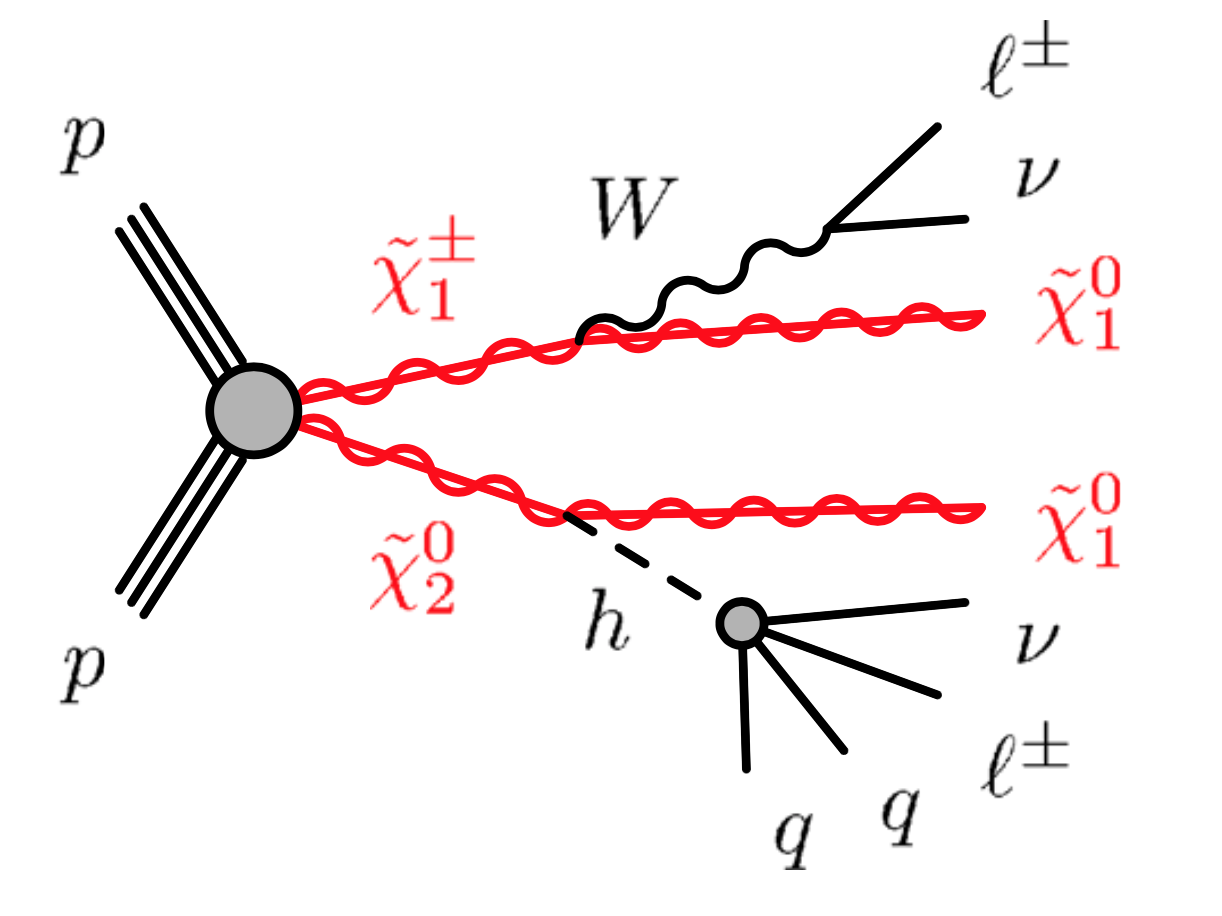
\includegraphics[width=0.3\textwidth]{data/photo/theory/signal_feynman.png}
\caption{The Feynman diagram for our Wh same-sign signal scenario.}
\end{figure}
\end{frame}

\begin{frame}{Our Signal Scenario : Decay Processes}
\begin{itemize}
\item The W boson will decay leptonically to one lepton (electron or muon) and one neutrino with the SM branching ratio : \\
$W{^\pm} \rightarrow \ell^{\pm} + \nu$
\item The Higgs boson $h$ will eventually decay to one lepton (electron or muon), quarks (i.e. jets) and neutrino(s) by various decay modes with the SM branching ratios. (For example, $h \rightarrow W^{+} W^{-} $ and $h \rightarrow \tau^{+} \tau^{-} $)
\item From now on, a lepton $\ell^{\pm}$ only refer to an electron or muon, but not $\tau$ lepton or neutrino.
\end{itemize}
\begin{figure}
\centering
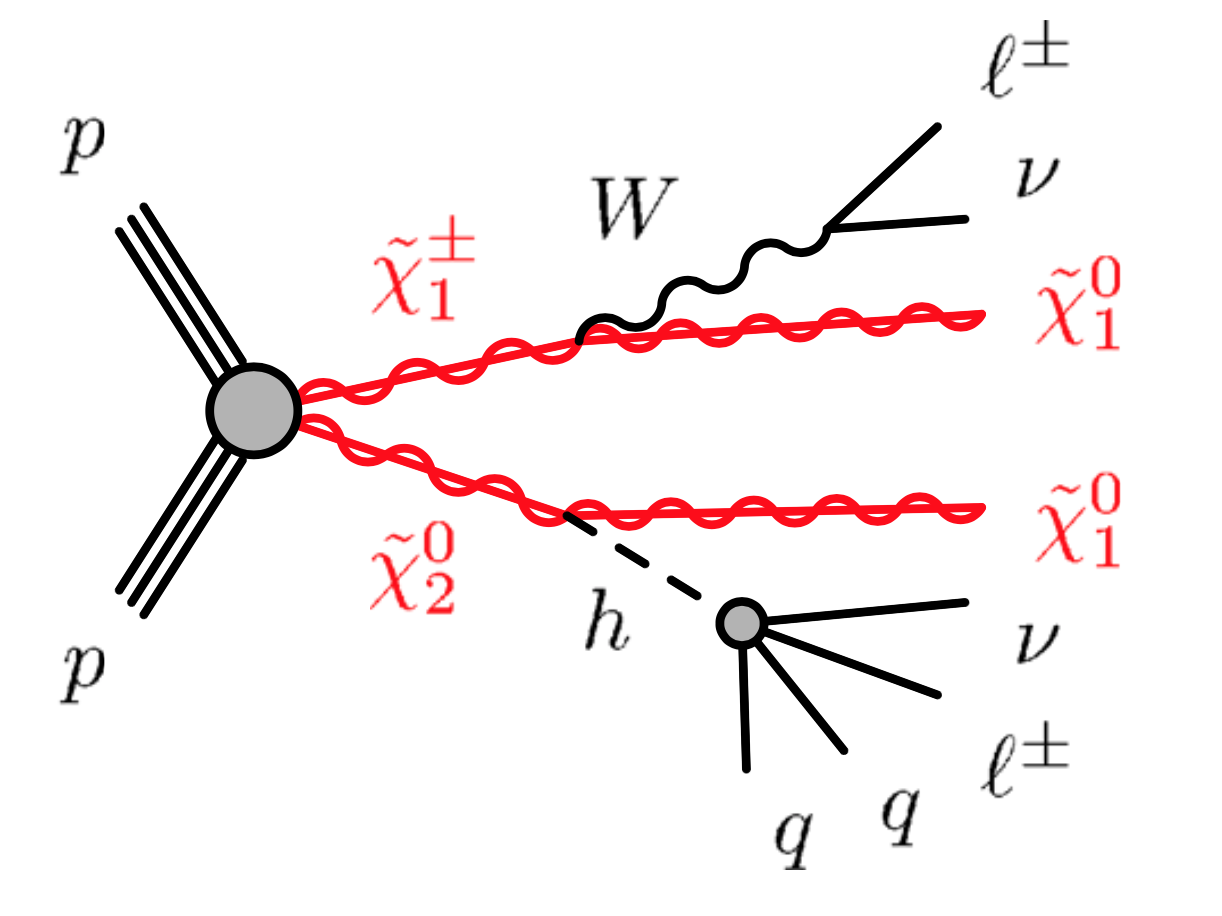
\includegraphics[width=0.3\textwidth]{data/photo/theory/signal_feynman.png}
\end{figure}
\end{frame}

\begin{frame}{Our Signal Scenario : Signal Signature in the Final State}
\begin{itemize}
\item In this thesis, we search for two same-sign(SS) leptons, in order to reduce the SM backgrounds.
\item A large missing energy is expected, due to the undetected neutralinos $\tilde{\chi}_1^0$ and neutrinos $\nu$.
\item Each quark will eventually become a particle shower within a narrow cone, called a jet, by the process of hadronization.
\item The mass difference between the two lightest neutralinos ($m_{\tilde{\chi}_2^0} - m_{\tilde{\chi}_1^0}$) should be larger than the Higgs mass ($\sim$ 125 GeV).
\end{itemize}
\begin{figure}
\centering
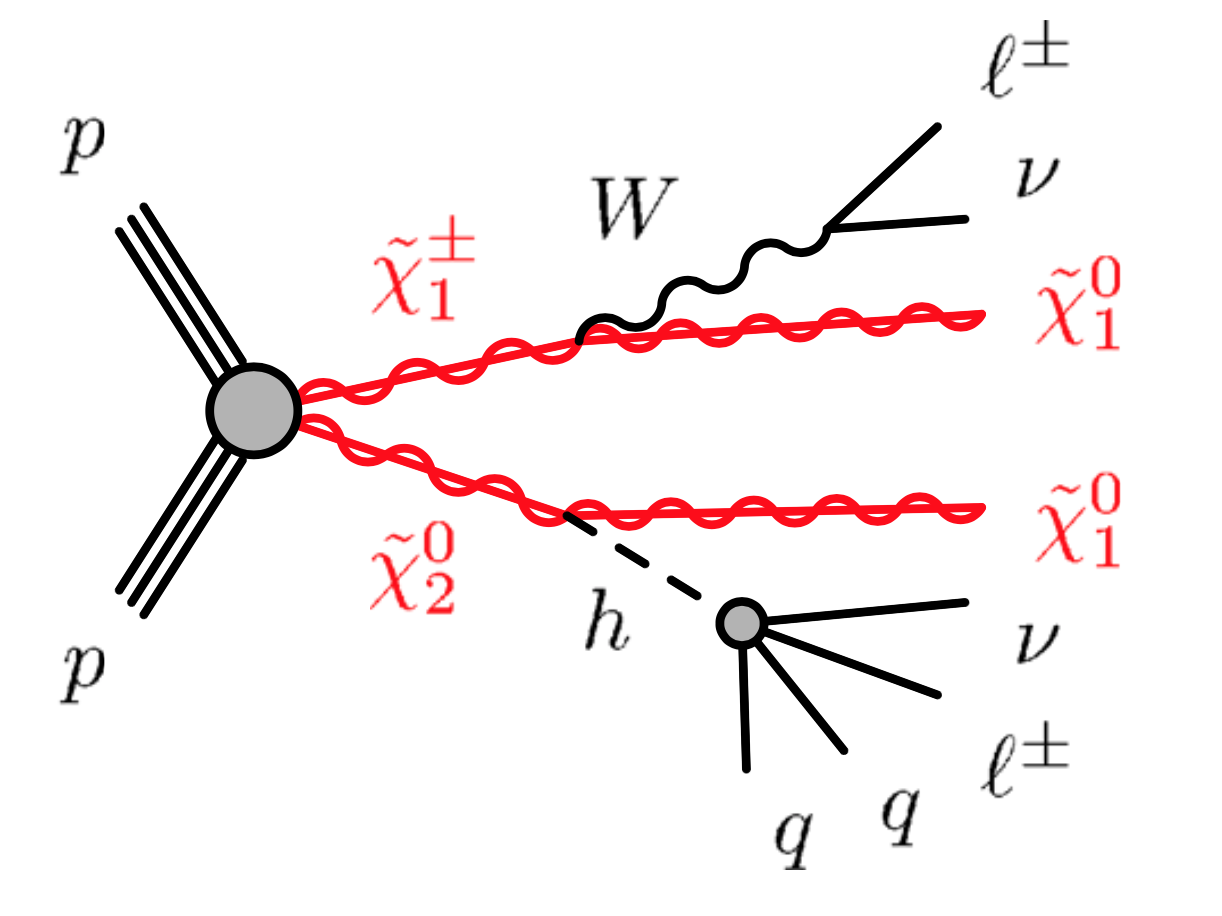
\includegraphics[width=0.3\textwidth]{data/photo/theory/signal_feynman.png}
\end{figure}
\end{frame}

\begin{frame}{Our Signal Scenario : Sensitive Region}
\begin{itemize}
\item If the mass difference ($m_{\tilde{\chi}_1^\pm , \tilde{\chi}_2^0} - m_{\tilde{\chi}_1^0}$) is slightly larger than the Higgs mass, it is called the compressed region.
\item In the compressed region, one of the lepton may have low energy, due to the low momentum of the Higgs boson, and hence it may not be detected.
\item In this case, only 2 out of 3 leptons are detected.
\item Our search channel would be more sensitive than the 3-leptons channel in the compressed region.
\end{itemize}
\end{frame}

\section{Experimental Setup}
\begin{frame}
\begin{center}
\huge
Experimental Setup
\end{center}
\end{frame}

\begin{frame}{Experimental Setup : LHC}
\begin{itemize}
\item The Large Hadron Collider (LHC) is the most powerful circular particle accelerator in the world.
\item Its circumference is 27 km.
\item Two beams of protons will be accelerated in opposite direction to centre-of-mass energy 13 TeV.
\item They will be finally collided at the ATLAS detector.
\end{itemize}
\begin{figure}
\centering
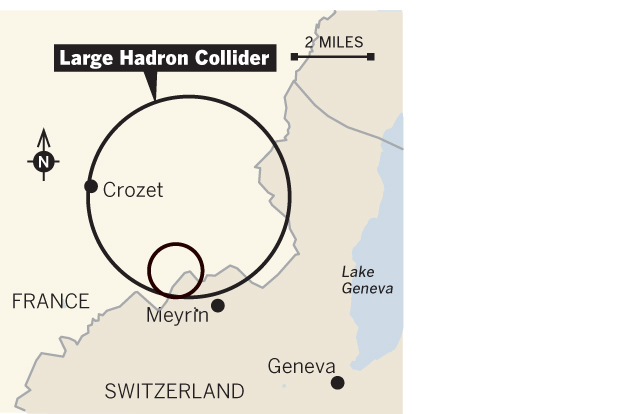
\includegraphics[width=0.6\textwidth]{data/photo/detector/LHC.jpg}
\end{figure}
\end{frame}

\begin{frame}{Experimental Setup : ATLAS detector}
\begin{figure}
\centering
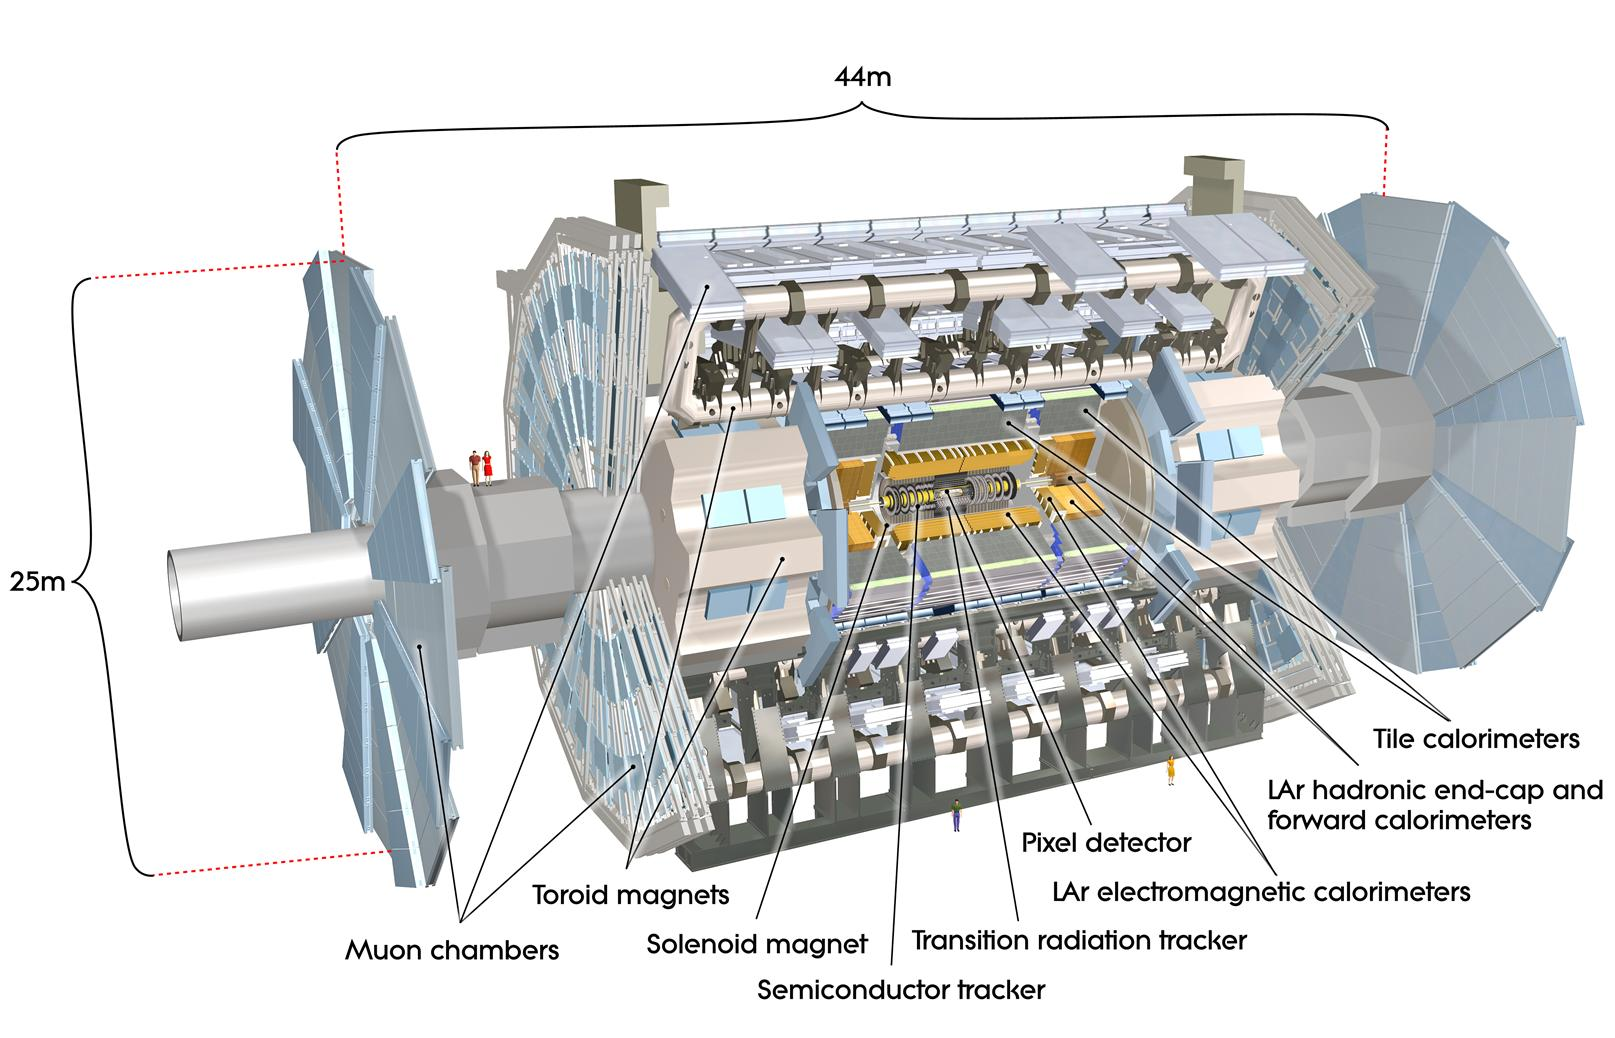
\includegraphics[width=\textwidth]{data/photo/detector/ATLAS.jpg}
\end{figure}
\end{frame}

\begin{frame}{Experimental Setup : ATLAS detector}
\begin{itemize}
\item The ATLAS detector consists of 3 main components:
\begin{enumerate}
\item Inner detector: It is a particle tracker. It measures the tracks of charged particles.
\item Calorimeter: It measures the energy of the particle and stops the particle. It consists of electromagnetic and hadronic calorimeters.
\item Muon spectrometer:  It is a particle tracker for muons.
\end{enumerate}
\end{itemize}
\begin{figure}
\centering
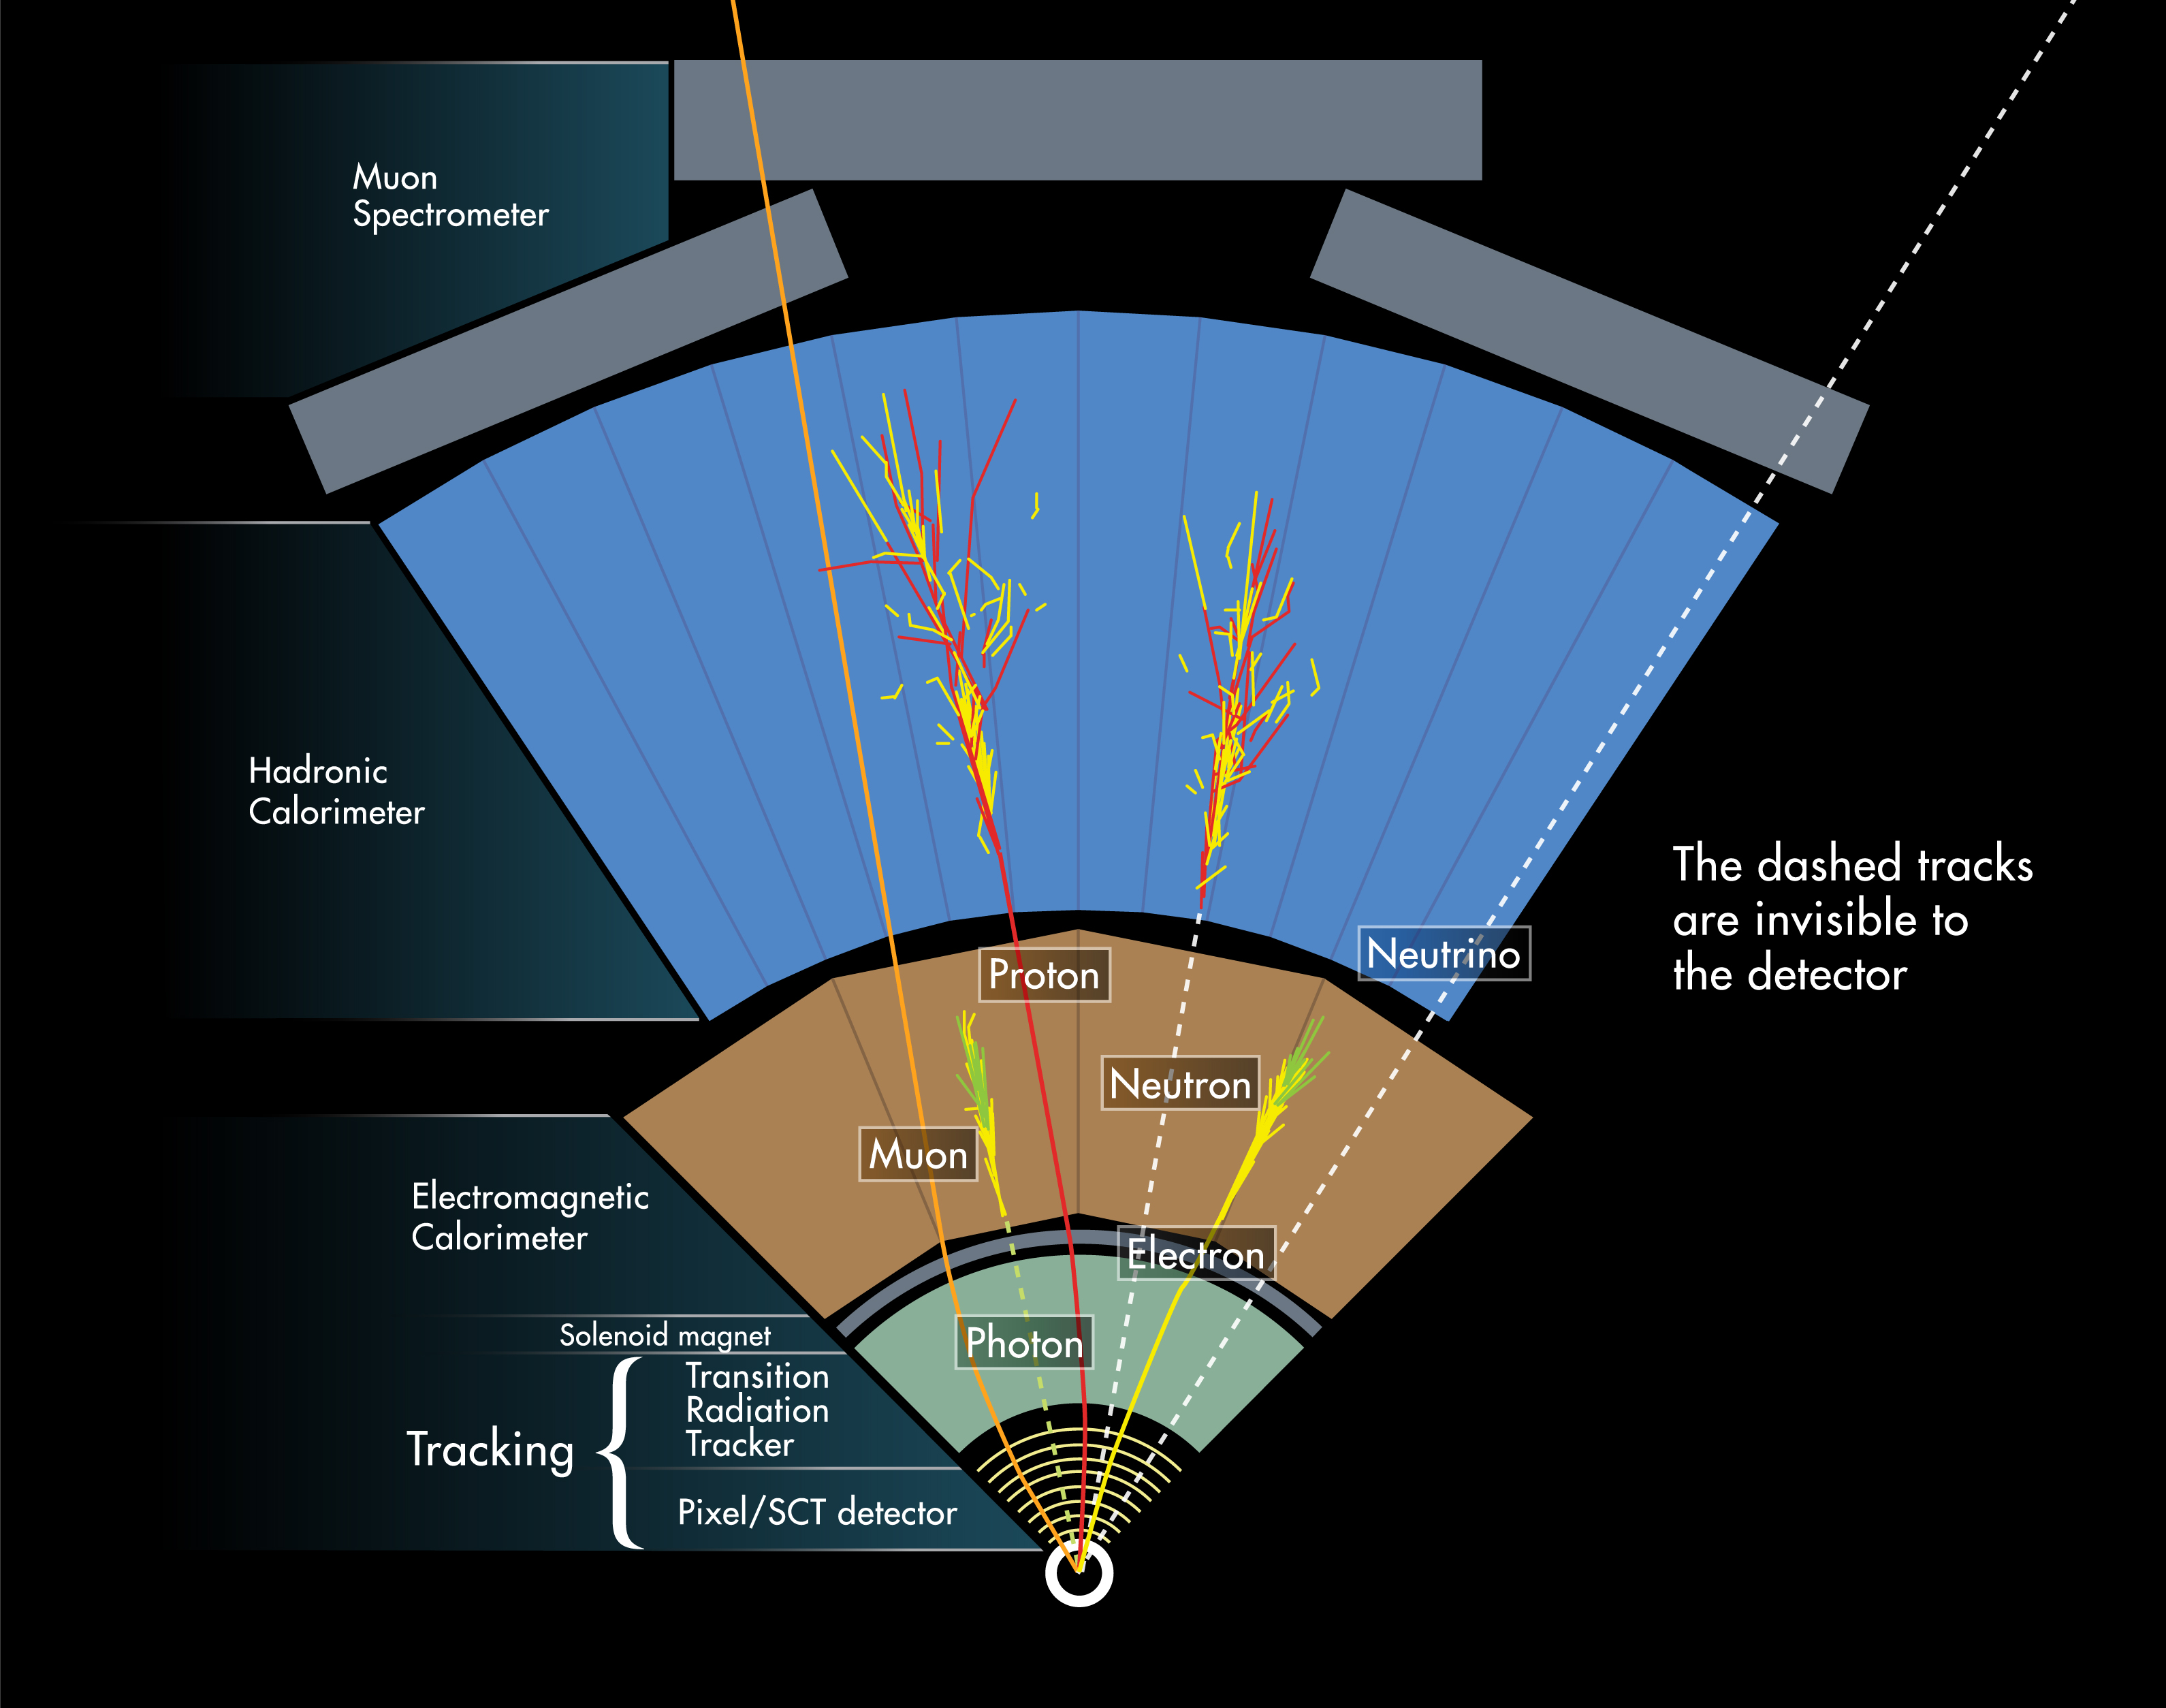
\includegraphics[width=0.5\textwidth]{data/photo/detector/ATLAS_particles.jpg}
\end{figure}
\end{frame}

\begin{frame}{Basic kinematic variables}
\begin{itemize}
\item The z-axis is in the proton beam direction.
\item The direction of the momentum $\bf{p}$ of the particle can by specified by the azimuthal angle $\phi$ and the polar angle $\theta$, as usual in the spherical coordinate system.
\end{itemize}
\begin{figure}
\centering
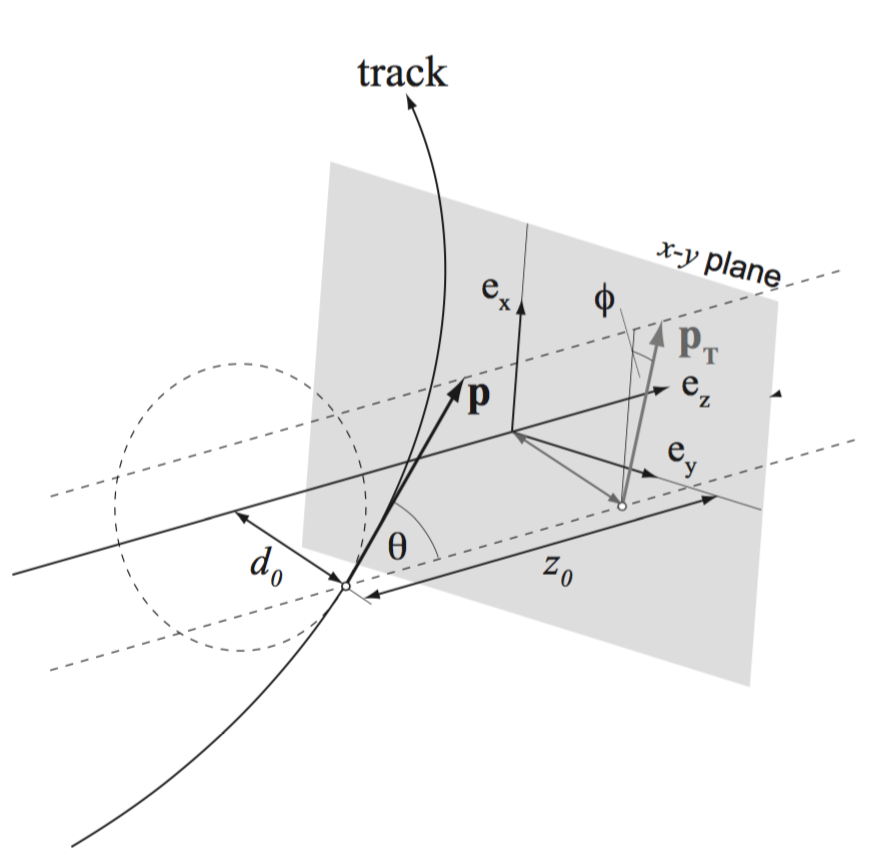
\includegraphics[width=0.4\textwidth]{data/photo/detector/impact_parameter.png}
\end{figure}
\end{frame}

\begin{frame}{Basic kinematic variables}
\begin{itemize}
\item The transverse momentum $\bf{p}_T$ is the projection of $\bf{p}$ onto the x-y plane. The magnitude of $\bf{p}_T$ is denoted by $p_T$
\begin{equation*}
p_T = \sqrt{p_x^2 + p_y^2}
\end{equation*}
\item $p_T^1$ and $p_T^2$ are $p_T$ of the two leptons, with $p_T^1 \geq p_T^2$. The lepton with larger $p_T$ is called the leading lepton, while the lepton with smaller $p_T$ is called the sub-leading lepton.
\end{itemize}
\begin{figure}
\centering
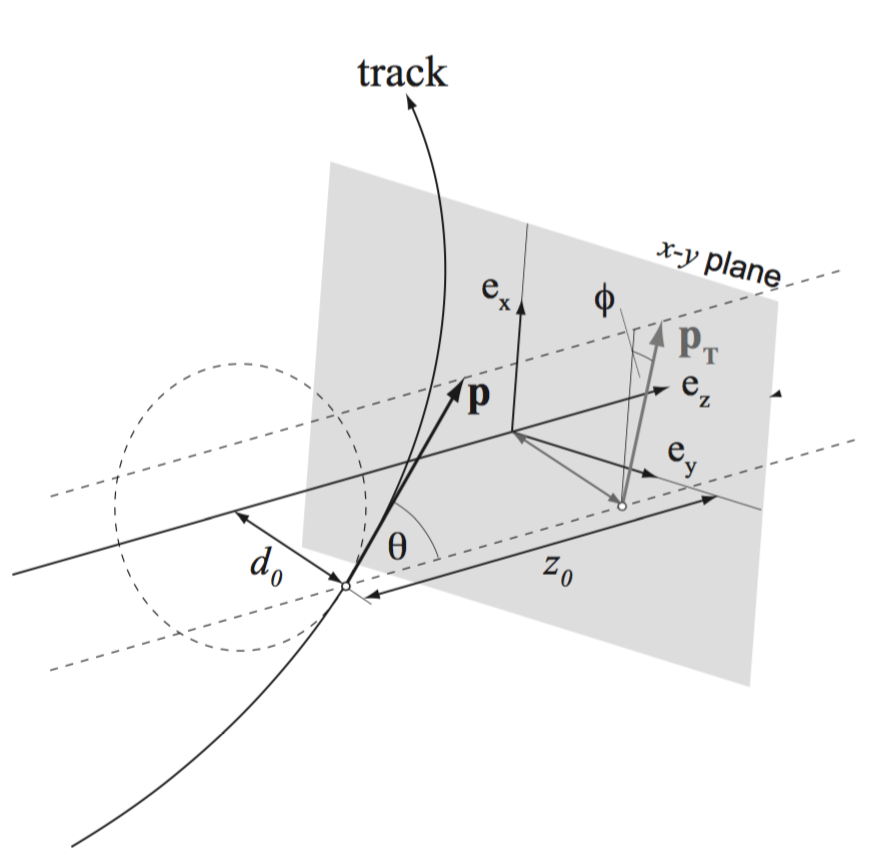
\includegraphics[width=0.4\textwidth]{data/photo/detector/impact_parameter.png}
\end{figure}
\end{frame}

\begin{frame}{Basic kinematic variables}
\begin{itemize}
\item The pseudorapidity $\eta$ is defined by
\begin{equation*}
\eta = - \ln \Big( \tan \frac{\theta}{2} \Big)
\end{equation*}
\item The angle separation $\Delta R$ of two particles is defined as:
\begin{equation*}
\Delta R = \sqrt{(\Delta \phi) ^2 + (\Delta \eta) ^2}  = \sqrt{(\phi_2 -\phi_1) ^2 + (\eta_2 - \eta_1) ^2}
\end{equation*}
\end{itemize}
\begin{figure}
\centering
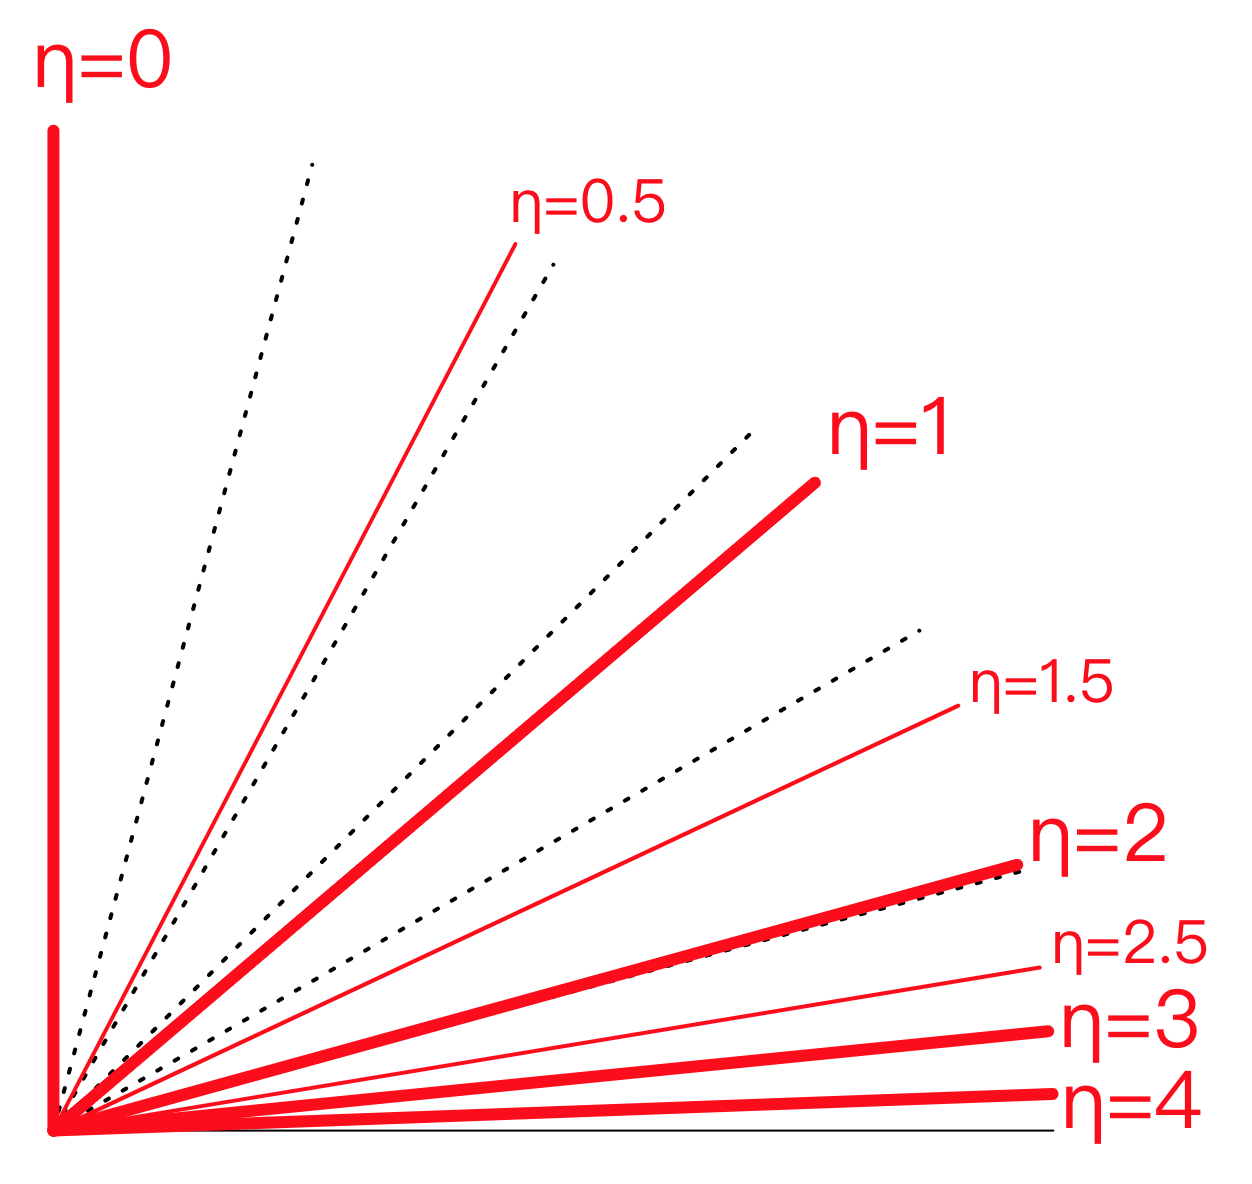
\includegraphics[width=0.3\textwidth]{data/photo/detector/pseudorapidity.png}
\end{figure}
\end{frame}

\begin{frame}{Challenges of Background Estimatation}
In order to search for SUSY, we need to understand the SM background very well.
\begin{enumerate}
\item Reducible SM background: They are due to the limitation of our detector and the wrong identification of the particle. There are two dominant reducible SM backgrounds, which are estimated by the data-driven method.
\begin{itemize}
\item Charge flip background
\item Fake lepton background (dominant background)
\end{itemize}
\item Irreducible SM background: They are estimated by Monte Carlo (MC)
\begin{itemize}
\item VV: WZ, WW, ZZ
\item tt+V
\item Rare: VVV, multitop, Higgs
\end{itemize}
\end{enumerate}
\end{frame}

\section{Charge Flip Background}
\begin{frame}
\begin{center}
\huge
Charge Flip Background
\end{center}
\end{frame}

\begin{frame}{Charge Flip Background : Sources}
\begin{itemize}
\item The charge flip background is due to the mis-identification of the sign of the charge of a lepton (mainly electron) in the reconstruction.
\item The sign of the charge is determined by the direction of the curvature of the track. The charge may be reversed, or flipped.
\end{itemize}
\begin{figure}
\centering
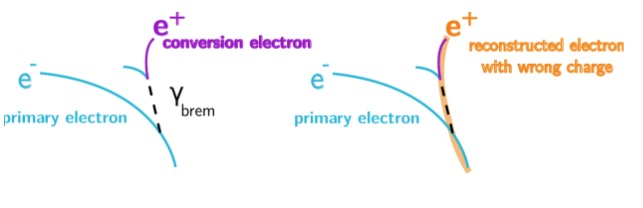
\includegraphics[width=0.4\textwidth]{data/photo/charge_flip/Brem.jpg}
\caption{Bremsstrahlung and $\gamma$ conversion.}
\end{figure}
\begin{figure}
\centering
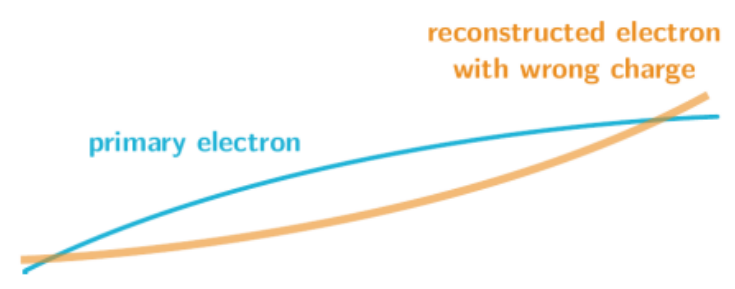
\includegraphics[width=0.3\textwidth]{data/photo/charge_flip/WrongTrack.png}
\caption{Track with high velocity}
\end{figure}
\end{frame}


\begin{frame}{Charge Flip Background : Charge Flip Rate}
\begin{itemize}
\item The probability that the charge of an electron is flipped is denoted by the charge-flip rate $\epsilon_i$, where the index i represents the dependency on the $p_T$ and $|\eta|$ of the electron.
\item The value of index i is defined by the index of the following grids in the table.

\begin{table}[htbp]
\centering
\begin{tabular}{|c|c|}
\hline
Variable & Boundary of the bins \\
\hline
$p_T$ (GeV) &  25, 60, 90, 130, 150, 1000 \\
\hline
$|\eta|$ & 0, 0.50, 1.00, 1.37, 1.52, 1.80, 2.00, 2.47 \\
\hline
\end{tabular}
\caption{Binning in $p_T$ and $|\eta|$ for the charge-flip rate $\epsilon_i$.}
\end{table}

\item The probability $p_{ij}$ that an OS data event becomes a SS data event (with the leading lepton in bin $i$ and the subleading lepton in bin $j$) is
\begin{equation*}
p_{ij} = (1 - \epsilon_i)\epsilon_j + (1 - \epsilon_j)\epsilon_i
\end{equation*}
\item It is called the charge flip weight.
\end{itemize}

\end{frame}

\begin{frame}{Charge Flip Background : Charge Flip Rate}
\begin{itemize}
\item The charge flip rates are measured by the likelihood method described in the next slide.
\item After getting the charge flip rates, the charge flip background can be estimated by applying the charge flip weights on all OS events in data.
\end{itemize}
\end{frame}


\begin{frame}{Charge Flip Background : Likelihood Method}
\begin{itemize}
\item The charge flip rate $\epsilon_i$ is measured by using the data in the control region, within the Z mass window cut of 80-100 GeV.
\item The events inside the Z mass window is then subtracted by the non-Zee processes, by using the sideband technique.
\item After the subtraction, the total number of event is denoted by $N^{ij}$, and the number of events with two same-sign leptons is denoted by $N^{ij}_{SS}$.
\item The expected value of $N^{ij}_{SS}$ is then given by $\lambda = N^{ij}p_{ij}$. And, if $N^{ij}_{SS}$ is described by a Poisson distribution, then
\end{itemize}
\begin{equation*}
P(N^{ij}_{SS} | N^{ij}, \epsilon_i, \epsilon_j) = \frac{(N^{ij}p_{ij})^{N^{ij}_{SS}} e^{-N^{ij}p_{ij}}}{N^{ij}_{SS}!}
\end{equation*}
\end{frame}

\begin{frame}{Charge Flip Background : Likelihood Method}
\begin{itemize}
\item Converting it to the likelihood function L and taking the negative natural log yields
\end{itemize}
\begin{equation*}
\begin{split}
-\ln L &= -\ln\prod_{ij} P(N^{ij}_{SS} | N^{ij}, \epsilon_i, \epsilon_j) \\
&= - \sum_{ij} \Big[ N^{ij}_{SS} \ln (N^{ij}[\epsilon_i (1-\epsilon_j) + (1-\epsilon_i) \epsilon_j]) \\
&- N^{ij}[\epsilon_i (1-\epsilon_j) + (1-\epsilon_i) \epsilon_j] \Big] + \text{constant}
\end{split}
\end{equation*}
\begin{itemize}
\item where the summation over $i$ and $j$ is taken over all $p_T$ and $|\eta|$ bins of both electrons.
\item By minimizing this likelihood, the charge-flip rate can be estimated.
\end{itemize}
\end{frame}

\begin{frame}{Charge Flip Background : Result for Charge Flip Rate}
\begin{figure}
\centering
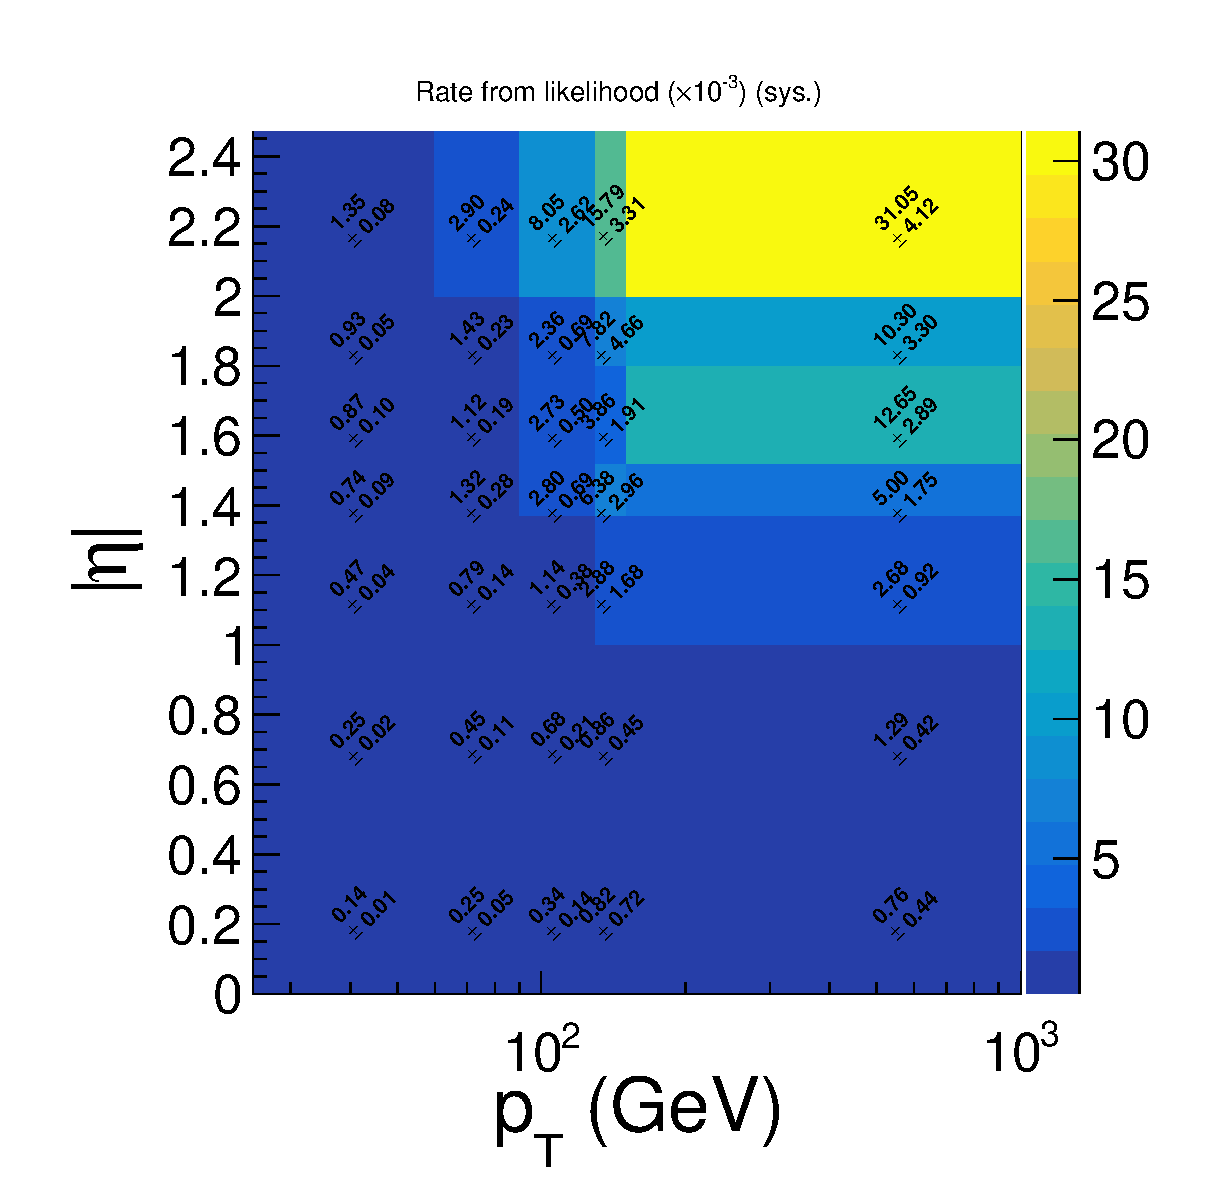
\includegraphics[width=0.6\textwidth]{data/plot/charge_flip/FitPlots/data_cf_rate_tot.eps}
\caption{The measured values of the charge-flip rate $\epsilon_i$ in data, with total uncertainties.}
\label{fig:charge_flip_data_tot}
\end{figure}
\end{frame}

\section{Fake Lepton Background}
\begin{frame}
\begin{center}
\huge
Fake Lepton Background
\end{center}
\end{frame}

\begin{frame}{Fake Lepton Background : Sources}
The source of the fake lepton is that other object (like jet and photon) is mis-identified as a lepton. Thay can be mainly classified into 3 types:
\begin{itemize}
\item Heavy-flavor fakes:
\begin{itemize}
\item leptons from the semi-leptonic decays of heavy-quark (b or c) hadrons.
\end{itemize}
\item Light-flavor fakes:
\begin{itemize}
\item leptons from the semi-leptonic decays of light-quark hadrons. \\ OR
\item It is due to mis-identification of light-quark hadrons.
\end{itemize}
\item photon conversion:
\begin{itemize}
\item leptons from the pair production of a photon
\end{itemize}
\end{itemize}
\end{frame}

\begin{frame}{Fake Lepton Background : Matrix Method}
\begin{itemize}
\item The fake leptons is estimated by the matrix method.
\item The probability that a real lepton passes the tight selection criteria (i.e. tight lepton) is denoted by the real efficiency $\epsilon$.
\item The probability that a real lepton does not pass the tight selection criteria (i.e. loose lepton) is denoted by $\bar{\epsilon} = 1 - \epsilon$.
\item The probability that a fake lepton passes the tight selection criteria (i.e. tight lepton) is denoted by the fake efficiency $f$.
\item The probability that a fake lepton does not pass the tight selection criteria (i.e. loose lepton) is denoted by $\bar{f} = 1 - f$.
\end{itemize}

\begin{equation*}
\left( \begin{array}{c}
N_T \\
N_L
\end{array} \right)
=
\left( \begin{array}{cc}
\epsilon & f \\
\bar{\epsilon} & \bar{f}
\end{array} \right)
\left( \begin{array}{c}
N_R \\
N_F
\end{array} \right)
\end{equation*}
\end{frame}

\begin{frame}{Fake Lepton Background : Matrix Method}
Suppose we know $\left( \begin{array}{c}
N_T \\
N_L
\end{array} \right)$, we can find $N_F$ by inverting the matrix.

\begin{equation*}
\left( \begin{array}{c}
0 \\
N_F
\end{array} \right)
=
\left( \begin{array}{cc}
0 & 0 \\
0 & 1
\end{array} \right)
\left( \begin{array}{c}
N_R \\
N_F
\end{array} \right)
=
\left( \begin{array}{cc}
0 & 0 \\
0 & 1
\end{array} \right)
\left( \begin{array}{cc}
\epsilon & f \\
\bar{\epsilon} & \bar{f}
\end{array} \right)^{-1}
\left( \begin{array}{c}
N_T \\
N_L
\end{array} \right)
\end{equation*}
Then, we can find the number of tight lepton due to the fake lepton, $N_T'$

\begin{equation*}
\left( \begin{array}{c}
N_T' \\
N_L'
\end{array} \right)
=
\left( \begin{array}{cc}
\epsilon & f \\
\bar{\epsilon} & \bar{f}
\end{array} \right)
\left( \begin{array}{c}
0 \\
N_F
\end{array} \right)
\end{equation*}

\begin{equation*}
=
\left( \begin{array}{cc}
\epsilon & f \\
\bar{\epsilon} & \bar{f}
\end{array} \right)
\left( \begin{array}{cc}
0 & 0 \\
0 & 1
\end{array} \right)
\left( \begin{array}{cc}
\epsilon & f \\
\bar{\epsilon} & \bar{f}
\end{array} \right)^{-1}
\left( \begin{array}{c}
N_T \\
N_L
\end{array} \right)
\end{equation*}
\end{frame}

\begin{frame}{Fake Lepton Background : Matrix Method}
We can generalize the one-lepton case to the two-leptons case.
\begin{equation*}
\left( \begin{array}{c}
N_{TT} \\
N_{TL} \\
N_{LT} \\
N_{LL}
\end{array} \right)
=
\left( \begin{array}{cccc}
\epsilon_1 \epsilon_2 & \epsilon_1 f_2 & f_1 \epsilon_2 & f_1 f_2 \\
\epsilon_1 \bar{\epsilon_2} & \epsilon_1 \bar{f_2} & f_1 \bar{\epsilon_2} & f_1 \bar{f_2} \\
\bar{\epsilon_1} \epsilon_2 & \bar{\epsilon_1} f_2 & \bar{f_1} \epsilon_2 & \bar{f_1} f_2 \\
\bar{\epsilon_1} \bar{\epsilon_2} & \bar{\epsilon_1} \bar{f_2} & \bar{f_1} \bar{\epsilon_2} & \bar{f_1} \bar{f_2}
\end{array} \right)
\left( \begin{array}{c}
N_{RR} \\
N_{RF} \\
N_{FR} \\
N_{FF}
\end{array} \right)
\end{equation*}
where $\epsilon_1$ is the probability that a leading real lepton passes the signal selection (i.e. tight lepton), $\epsilon_2$ is the probability that a subleading real lepton passes the signal selection (i.e. tight lepton), etc.
\end{frame}

\begin{frame}{Fake Lepton Background : Matrix Method}
Similarly, we can find the number of tight-tight leptons due to the fake leptons, $N_{TT}'$

\begin{equation*}
\left( \begin{array}{c}
N_{TT}' \\
N_{TL}' \\
N_{LT}' \\
N_{LL}'
\end{array} \right)
=
\left( \begin{array}{cccc}
\epsilon_1 \epsilon_2 & \epsilon_1 f_2 & f_1 \epsilon_2 & f_1 f_2 \\
\epsilon_1 \bar{\epsilon_2} & \epsilon_1 \bar{f_2} & f_1 \bar{\epsilon_2} & f_1 \bar{f_2} \\
\bar{\epsilon_1} \epsilon_2 & \bar{\epsilon_1} f_2 & \bar{f_1} \epsilon_2 & \bar{f_1} f_2 \\
\bar{\epsilon_1} \bar{\epsilon_2} & \bar{\epsilon_1} \bar{f_2} & \bar{f_1} \bar{\epsilon_2} & \bar{f_1} \bar{f_2}
\end{array} \right)
\left( \begin{array}{cccc}
0 & 0 & 0 & 0 \\
0 & 1 & 0 & 0 \\
0 & 0 & 1 & 0 \\
0 & 0 & 0 & 1
\end{array} \right)
\end{equation*}

\begin{equation*}
\left( \begin{array}{cccc}
\epsilon_1 \epsilon_2 & \epsilon_1 f_2 & f_1 \epsilon_2 & f_1 f_2 \\
\epsilon_1 \bar{\epsilon_2} & \epsilon_1 \bar{f_2} & f_1 \bar{\epsilon_2} & f_1 \bar{f_2} \\
\bar{\epsilon_1} \epsilon_2 & \bar{\epsilon_1} f_2 & \bar{f_1} \epsilon_2 & \bar{f_1} f_2 \\
\bar{\epsilon_1} \bar{\epsilon_2} & \bar{\epsilon_1} \bar{f_2} & \bar{f_1} \bar{\epsilon_2} & \bar{f_1} \bar{f_2}
\end{array} \right)^{-1}
\left( \begin{array}{c}
N_{TT} \\
N_{TL} \\
N_{LT} \\
N_{LL}
\end{array} \right)
\end{equation*}
\end{frame}

\begin{frame}{Fake Lepton Background : Results of Fake Efficiencies}
The method for measuring the fake efficiencies is described in the backup slides.
\begin{figure}
\begin{columns}

\begin{column}{0.5\textwidth}
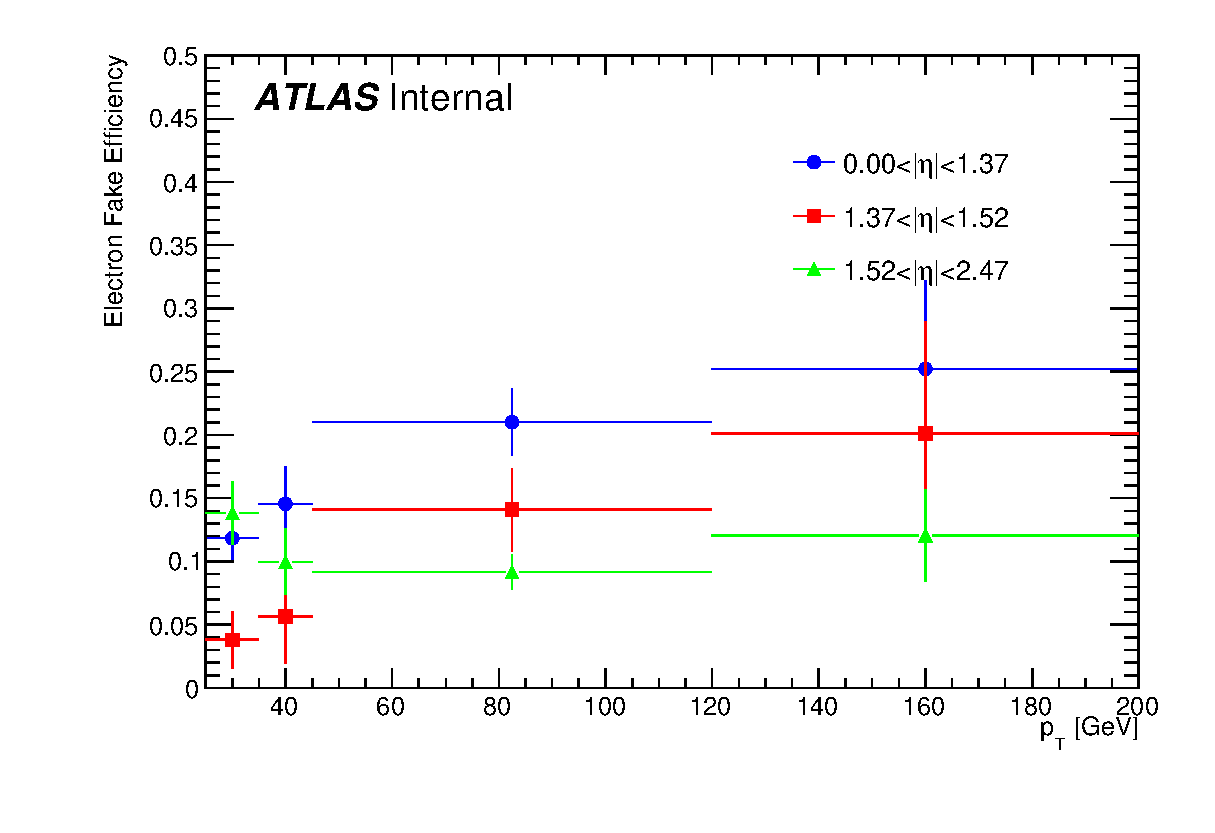
\includegraphics[width=\textwidth]{data/plot/getFakeEffs/El_hEff.eps}
\caption{Electron fake efficiency}
\end{column}

\begin{column}{0.5\textwidth}
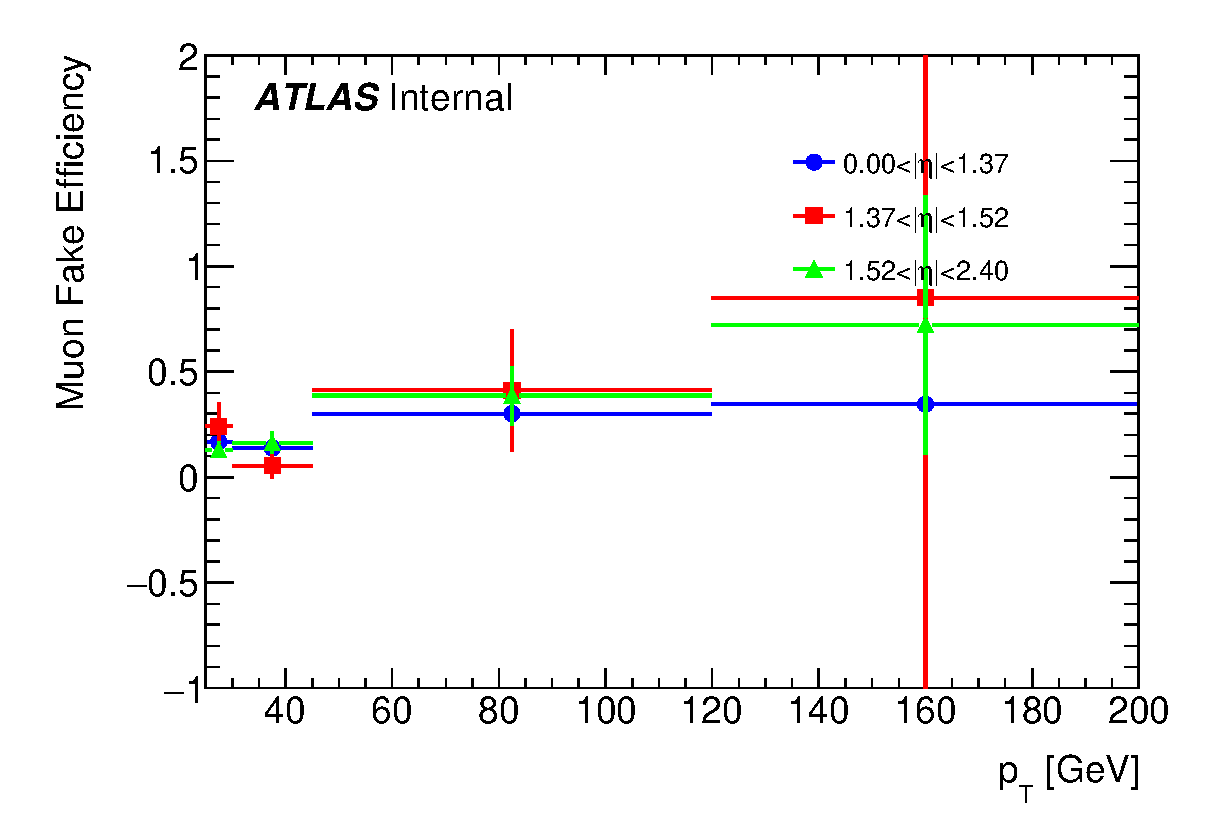
\includegraphics[width=\textwidth]{data/plot/getFakeEffs/Mu_hEff.eps}
\caption{Muon fake efficiency}
\end{column}

\end{columns}
\end{figure}
\end{frame}

\section{Signal Region}
\begin{frame}
\begin{center}
\huge
Signal Region
\end{center}
\end{frame}

\begin{frame}{Signal Region: Challenges}
Estimation of the signal sensitivity
\begin{itemize}
\item Cross section for our signal $\sim 0.1$ pb
\item Total luminosity in one year $\sim 10^4$ pb$^{-1}$
\item Expected number of signal events in one year $\sim 10^3$
\end{itemize}
\begin{itemize}
\item Time interval between each collision $= 25$ ns
\item Total number of collisions in one year $\sim 10^{15}$
\item The probability to have a signal event $\sim 10^{-12}$
\item Conclusion: the SUSY signal is very rare.
\end{itemize}
\end{frame}

\begin{frame}{Signal Region : Strategy}
In order to extract the signal, the following strategies are used.
\begin{itemize}
\item A trigger system are used when taking the data (online), to only store the interested events in the disk. \\
(40 MHz $\rightarrow$ 100 kHz $\rightarrow$ 1 kHz)
\item Some discriminant variables (based on the kinematic variables) are defined, to help distinguish the signal and the background.
\item Two dedicated signal regions are defined (SRjet1 and SRjet23) based on the discriminant variables, to maximize the signal sensitivity.
\end{itemize}
\end{frame}

\begin{frame}{Signal Region : discriminant variable}
\begin{itemize}
\item $n_{\text{jets}}$: Number of signal jets:
\item $n_{\text{b-jets}}$: Number of $b$-jets (jet from b quark).
\item $\Delta \eta_{ll}$ is designed to estimate the angle between the two leptons.
\begin{equation*}
\Delta \eta_{ll} = |\eta_{1} - \eta_{2}|
\end{equation*}
\item $m_{\text{eff}}$ is designed to estimate the total energy and momentum of the charginos $\tilde{\chi}_1^\pm$ and neutralinos $\tilde{\chi}_2^0$.
\begin{equation*}
m_{\text{eff}} = p_T^1 + p_T^2 + E_T^{\text{miss}} + \sum_{\text {signal jets}} p_T
\end{equation*}
\item $m_{ll}$: The invariant mass of the 4-momentum sum of the two leptons
\begin{equation*}
(m_{ll})^2 = (p_1 + p_2)^2
\end{equation*}
\end{itemize}
\end{frame}

\begin{frame}{Signal Region : discriminant variable}
\begin{itemize}
\item The missing momentum ${\bf p}^{\text{miss}}$ due to undetected particles is defined by
\begin{equation*}
{\bf p}^{\text{miss}} = - \sum_{\text{All detected particles}}{\bf p}
\end{equation*}
\item $E_{T}^{\text{miss}}$ or MET: The transverse missing erengy is designed to estimate the missing energy from the undetected particles.
\begin{equation*}
E_{T}^{\text{miss}} = |{\bf p}_T^{\text{miss}}| = \sqrt{ (p_x^{\text{miss}})^2 + (p_y^{\text{miss}})^2}
\end{equation*}
\end{itemize}
\end{frame}

\begin{frame}{Signal Region : discriminant variable}
\begin{itemize}
\item $m_T$: It is designed to reconstruct the mass of the W boson.
\begin{equation*}
m_T = \sqrt{ 2 p_T^1 E_T^{\text{miss}} ( 1 - \cos{\Delta\phi} ) }
\end{equation*}
where $\Delta\phi$ is the azimuthal angle between the leading lepton and the missing transverse momentum.
\item $m_{T2}$: It is designed to set a lower bound on the masses of charginos $\tilde{\chi}_1^\pm$ and neutralinos $\tilde{\chi}_2^0$.
\begin{equation*}
m_{T2} = \min_{{\bf q}_T} \Bigg[ \max \bigg( m_T( {\bf p}_T^1, {\bf q}_T ), m_T( {\bf p}_T^2, {\bf p}_T^{\text{miss}} - {\bf q}_T ) \bigg) \Bigg]
\end{equation*}
\begin{equation*}
m_T( {\bf p}_T, {\bf q}_T ) = \sqrt{ 2 p_T q_T ( 1 - \cos{\Delta\phi} ) }
\end{equation*}
\end{itemize}
\end{frame}

\begin{frame}{Signal Region : discriminant variable}
\begin{itemize}
\item $m_{lj}$ or $m_{ljj}$: It is designed to reconstruct the mass of the Higgs boson.
\begin{equation*}
p_{\text{jet-system}} =
\left\{
\begin{array}{ll}
p_{\text{jet1}} &\text{ for SRjet1 (1 jet)}\\
p_{\text{jet1}} + p_{\text{jet2}} &\text{ for SRjet23 (2 or 3 jets)}
\end{array} \right.
\end{equation*}
\begin{equation*}
p_{\text{closest-lepton}} =
\left\{
\begin{array}{ll}
p_{\ell 1} &\text{ if } \Delta R(p_{\ell 1},p_{\text{jet-system}}) \leq \Delta R(p_{\ell 2},p_{\text{jet-system}}) \\
p_{\ell 2} &\text{ if } \Delta R(p_{\ell 1},p_{\text{jet-system}}) > \Delta R(p_{\ell 2},p_{\text{jet-system}})
\end{array} \right.
\end{equation*}
\begin{equation*}
(m_{lj(j)})^2 = (p_{\text{closest-lepton}} + p_{\text{jet-system}})^2
\end{equation*}
\end{itemize}
\end{frame}

\begin{frame}{Signal Region : Pre-selection}
\begin{itemize}
\item Signal Region(SR) is a set of cuts of the discriminant variables, such that the signal sensitivity is high.
\item By trying different sets of cuts, the signal region with the highest signal sensitivity can be found. This process is called the signal region optimization.
\item In the SR optimization, the MC signal and background are used to study the expected sensitivity.
\end{itemize}
The following cuts are the pre-selection, before the signal region optimization.
\begin{itemize}
\item Exactly 2 leptons with $p_T > 25$ GeV.
\item Electron: $|\eta| < 2.47$ ; Muon: $|\eta| < 2.4$
\item The two leptons are same-sign in electric charge (SS).
\item $n_{\text{b-jets}} = 0$, to reduce the SM background from top quark.
\item Two signal regions: SRjet1 with $n_{\text{jets}} = 1$, SRjet23 with $n_{\text{jets}} = 2$ or $3$.
\end{itemize}
\end{frame}

\begin{frame}{Signal Region : Pre-selection plots}
\Wider{
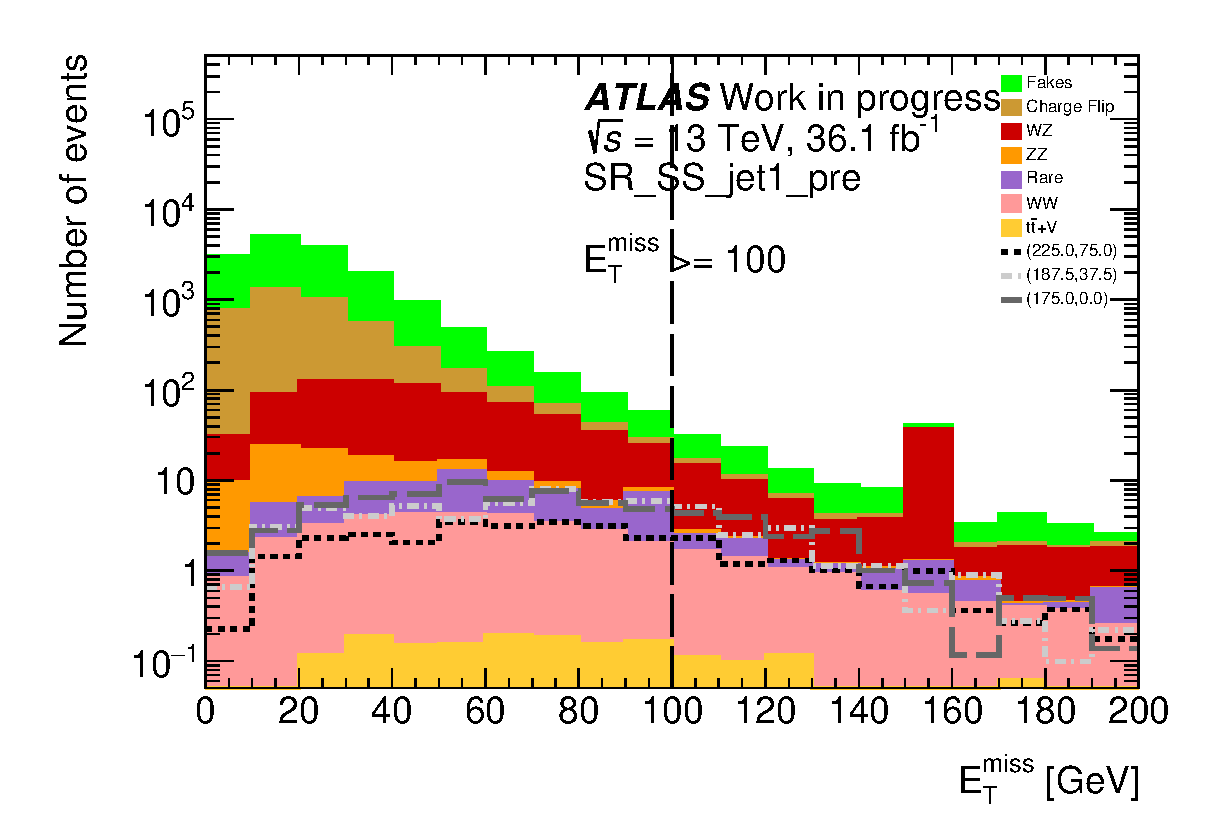
\includegraphics[width=0.49\textwidth]{MET_SR_SS_jet1_pre}
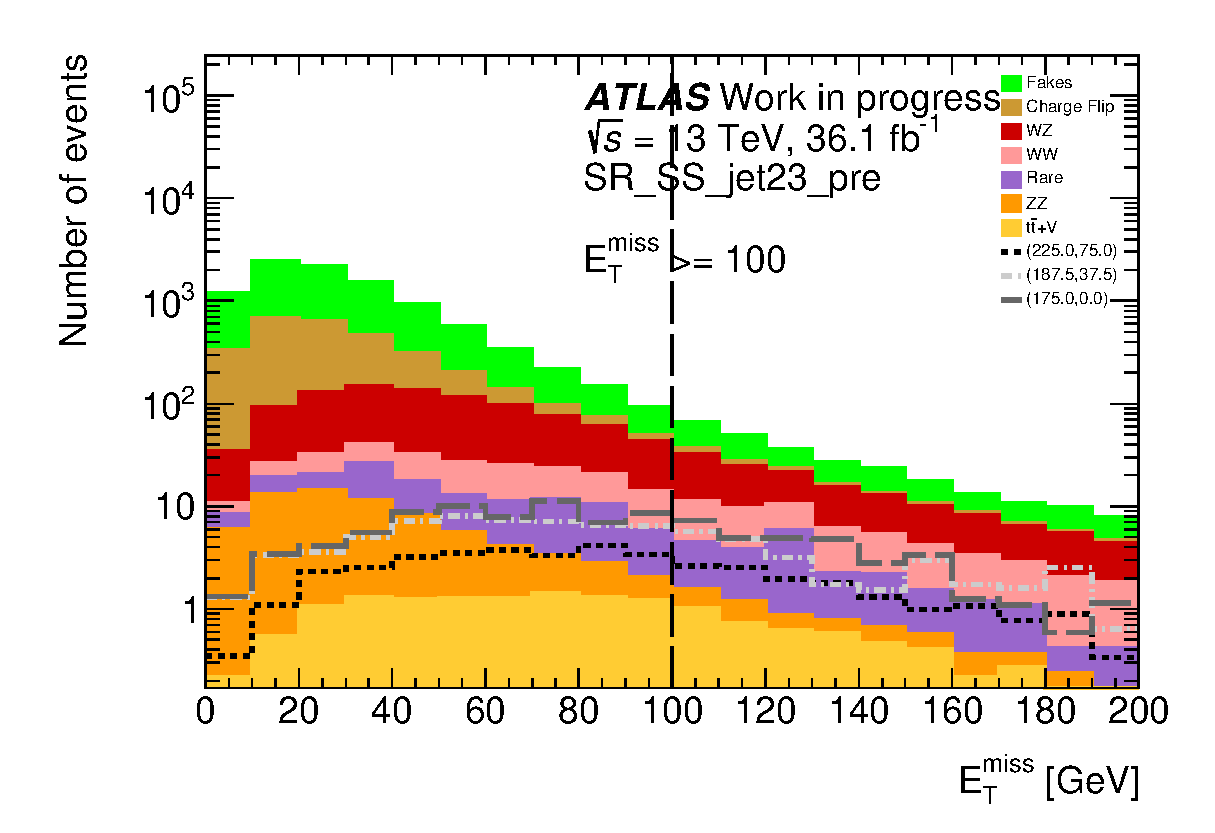
\includegraphics[width=0.49\textwidth]{MET_SR_SS_jet23_pre}
}
\end{frame}

\begin{frame}{Signal Region : Optimizied Event Selection}
\begin{tabular}{|c|c|c|}
\hline
& SRjet1 & SRjet23 \\
\hline
$n_{jets}$ & 1 & 2 or 3 \\
\hline
Leading lepton $p_T$ [GeV] & $\geq 25$ & $\geq 25$ \\
\hline
Sub-leading lepton $p_T$ [GeV] & $\geq 25$ & $\geq 25$ \\
\hline
$|\Delta\eta_{ll}|$ & $<1.5$ & - \\
\hline
$E_{\text{T}}^{\text{miss}}$ [GeV] & $\geq 100$ & $\geq 100$ \\
\hline
$m_{\text{eff}}$ [GeV] & $\geq 260$ & $\geq 240$ \\
\hline
$m_{\text{T}}^{l1}$ [GeV] & $\geq 140$ & $\geq 120$ \\
\hline
$m_{lj}$/$m_{ljj}$ [GeV] & $<180$ & $<130$ \\
\hline
$m_{T2}$ [GeV] & $\geq 80$ & $\geq 70$ \\
\hline

\end{tabular}
\end{frame}

\begin{frame}{Signal Region : Expected Yields and Sensitivity}
\begin{table}[htbp]
\centering
\tiny

\begin{columns}

\begin{column}{0.5\textwidth}
\begin{tabular}{|c|c|c|}
\hline
& Number of events & Significance \\
\hline
Fakes & $3.295\pm0.819$ & \\
\hline
WZ & $2.176\pm0.398$ & \\
\hline
charge flip & $0.472\pm0.053$ & \\
\hline
Rare & $0.444\pm0.111$ & \\
\hline
WW & $0.166\pm0.023$ & \\
\hline
$t\bar{t}+V$ & $0.125\pm0.046$ & \\
\hline
ZZ & $0.055\pm0.028$ & \\
\hline
Total BG & $6.733\pm0.921$ & \\
\hline
(225.0,75.0) & $3.33\pm0.60$ &$ \bf 0.74$\\
\hline
(187.5,37.5) & $3.77\pm0.95$ &$0.86$\\
\hline
(175.0,0.0) & $4.29\pm0.73$ &$0.98$\\
\hline

\end{tabular}
\caption{\tiny Yields in SRjet1}
\end{column}

\begin{column}{0.5\textwidth}
\begin{tabular}{|c|c|c|}
\hline
& Number of events & Significance \\
\hline
WZ & $1.849\pm0.273$ & \\
\hline
Fakes & $1.765\pm0.709$ & \\
\hline
Rare & $0.731\pm0.195$ & \\
\hline
WW & $0.514\pm0.037$ & \\
\hline
charge flip & $0.267\pm0.029$ & \\
\hline
$t\bar{t}+V$ & $0.142\pm0.031$ & \\
\hline
ZZ & $0.067\pm0.025$ & \\
\hline
Total BG & $5.335\pm0.787$ & \\
\hline
(225.0,75.0) & $2.35\pm0.34$ &$0.57$\\
\hline
(187.5,37.5) & $4.72\pm0.74$ &$\bf 1.26$\\
\hline
(175.0,0.0) & $8.60\pm1.51$ &$2.24$\\
\hline

\end{tabular}
\caption{\tiny Yields in SRjet23}
\end{column}

\end{columns}
\end{table}
\end{frame}

\begin{frame}{Signal Region : N-1 plots}
\Wider{
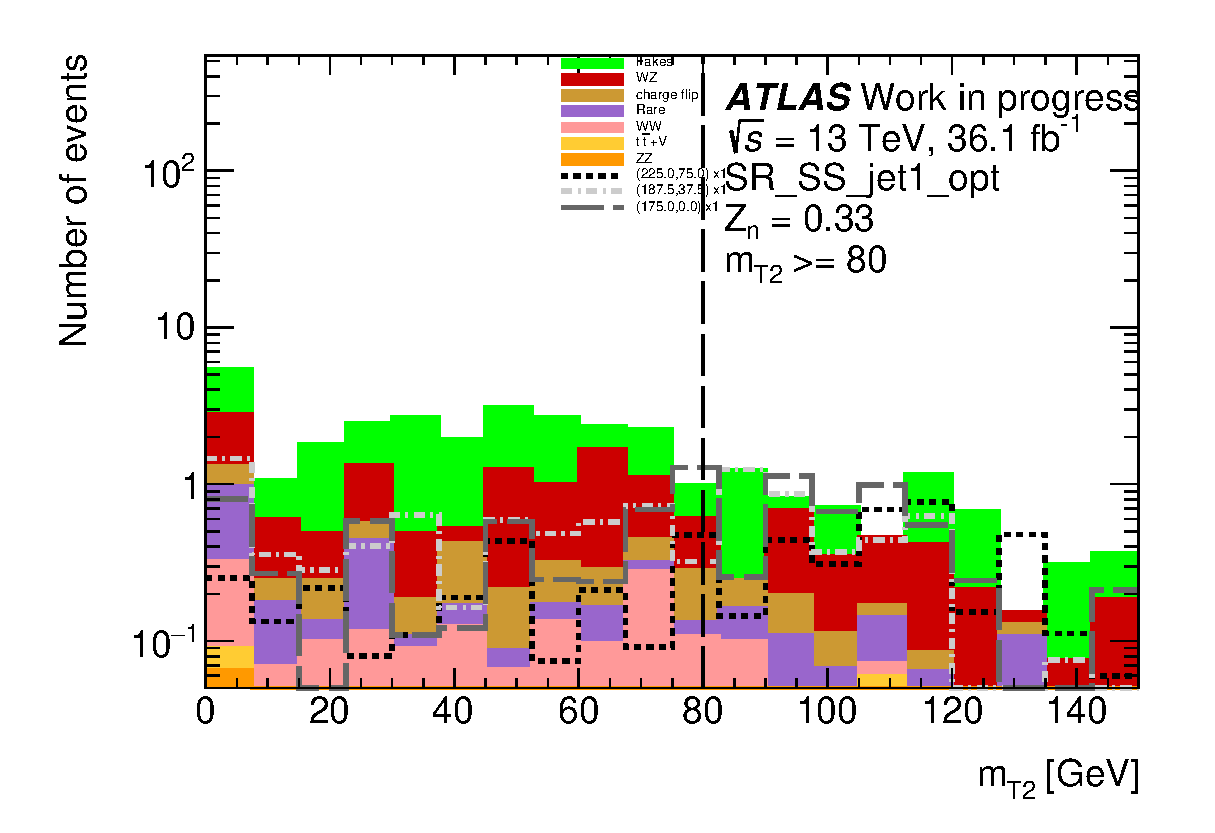
\includegraphics[width=0.49\textwidth]{mTtwo_SR_SS_jet1_opt_0}
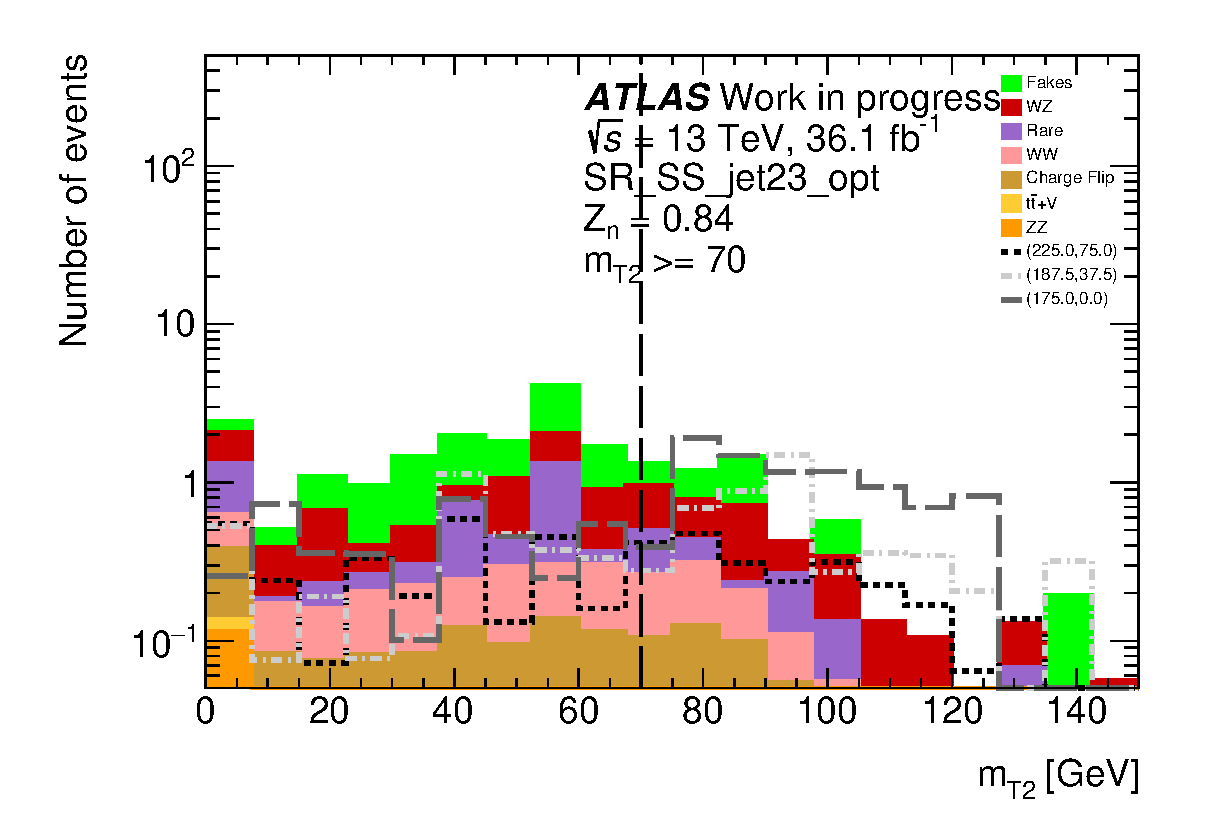
\includegraphics[width=0.49\textwidth]{mTtwo_SR_SS_jet23_opt_0}
}
\end{frame}

\section{Validation Region}
\begin{frame}
\begin{center}
\huge
Validation Region
\end{center}
\end{frame}

\begin{frame}{Validation Region: Introduction}
\begin{itemize}
\item The validation region(VR) is designed to ensure that the estimation of background is reliable.
\item Method: The backgrounds are compared with the data, to see whether they agree with each other.
\item One VR is defined for each SR: VRjet1 and VRjet23.
\end{itemize}
There are three requirements for the validation regions:
\begin{itemize}
\item The signal contribution should be small.
\item The validation region is orthogonal to the corresponding signal region.
\item The background composition is similar to the corresponding signal region.
\end{itemize}
\end{frame}

\begin{frame}{Validation Region: Method}
\begin{itemize}
\item In order to make the VR orthogonal to its SR, $E_T^{\text{miss}}$/$m_{T}$ cut is inverted.
\item Adjust its lower cut, to have a similar background composition as in its SR.
\item Invert the $m_{lj}$/$m_{ljj}$ cut, to reduce the signal.
\item Remove $m_{T2}$ and $m_{\text{eff}}$ cuts, to increase statistics.
\end{itemize}
\begin{table}[htbp]
\begin{center}
\begin{tabular}{|c|c|c|}
\hline
Cut & VRjet1 & VRjet23 \\
\hline
\hline
$n_{\text{jets}}$               & 1                             & $[2,3]$ \\
$\Delta \eta_{ll}$              & $<1.5$                        & $-$ \\
$E_T^{\text{miss}}$ [GeV]       & \textcolor{red}{ $[70,100]$ } & $>100$ \\
$m_T$ [GeV]                     & $>140$                        & \textcolor{red}{$[65,120]$} \\
$m_{\text{eff}}$ [GeV]          & $\textcolor{red}{-}$          & $>240$ \\
$m_{lj(j)}$ [GeV]               & \textcolor{red}{$>130$}       & \textcolor{red}{$>130$} \\
$m_{T2}$ [GeV]                  & $\textcolor{red}{-}$          & $\textcolor{red}{-}$ \\
\hline
\end{tabular}
\end{center}
\end{table}
\end{frame}

\begin{frame}{Validation Region: Yield}
\begin{table}
\begin{center}
\begin{tabular}{|l|c|c|}
\hline
\hline
Process & VRjet1 & VRjet23 \\
\hline
\hline
Rare        & $0.775\pm 0.389^{+0.661}_{-0.362}$ & $2.469 \pm 0.674^{+0.998} _{-0.899}$ \\
$t\bar{t}V$ & $0.039\pm 0.013^{+0.018}_{-0.012}$ & $0.959 \pm 0.082^{+0.152} _{-0.146}$ \\
ZZ          & $0.298\pm 0.060^{+0.089}_{-0.063}$ & $0.247 \pm 0.045^{+0.113} _{-0.047}$ \\
WZ          & $4.909\pm 0.530^{+0.960}_{-0.899}$ & $19.325\pm 0.643^{+4.393} _{-4.346}$ \\
WW          & $0.801\pm 0.051^{+0.123}_{-0.060}$ & $10.477\pm 0.176^{+0.796} _{-0.726}$ \\
Charge flip & $1.997\pm 0.128^{+0.260}_{-0.260}$ & $2.065 \pm 0.085^{+0.166} _{-0.166}$ \\
Fakes       & $8.021\pm 1.390^{+5.806}_{-5.806}$ & $19.990\pm 2.013^{+13.461}_{-13.461}$ \\
\hline
Total BG      & $16.839\pm 1.545^{+5.915}_{-5.912}$ & $55.534\pm 2.228^{+14.396}_{-14.332}$ \\
\hline
\hline
Data        & $17$ & $54$ \\
\hline
\hline
\end{tabular}
\caption{The uncertainties include the statistical and systematic uncertainties.}
\label{tab:VR_yields}
\end{center}
\end{table}
The distribution plots for different variables are in the backup slides.
\end{frame}

\section{Results}
\begin{frame}
\begin{center}
\huge
Results
\end{center}
\end{frame}

\begin{frame}{Results: Observed Events}
\begin{itemize}
\item The observed events are consistent with the SM.
\end{itemize}
\begin{table}[htbp]
\centering

\begin{columns}

\begin{column}{0.5\textwidth}
\begin{tabular}{|c|c|c|}
\hline
& Number of events \\
\hline
Fakes & $3.295\pm2.100$ \\
\hline
WZ & $2.176\pm0.398$ \\
\hline
charge flip & $0.472\pm0.053$ \\
\hline
Rare & $0.444\pm0.111$ \\
\hline
WW & $0.166\pm0.023$ \\
\hline
$t\bar{t}+V$ & $0.125\pm0.046$ \\
\hline
ZZ & $0.055\pm0.028$ \\
\hline
Total BG & $6.733\pm2.142$ \\
\hline
\hline
Data & 2 \\
\hline

\end{tabular}
\caption{Yields in SRjet1}
\end{column}

\begin{column}{0.5\textwidth}
\begin{tabular}{|c|c|c|}
\hline
& Number of events \\
\hline
WZ & $1.849\pm0.273$ \\
\hline
Fakes & $1.765\pm1.460$ \\
\hline
Rare & $0.731\pm0.195$ \\
\hline
WW & $0.514\pm0.037$ \\
\hline
charge flip & $0.267\pm0.029$ \\
\hline
$t\bar{t}+V$ & $0.142\pm0.031$ \\
\hline
ZZ & $0.067\pm0.025$ \\
\hline
Total BG & $5.335\pm1.499$ \\
\hline
\hline
Data & 8 \\
\hline

\end{tabular}
\caption{Yields in SRjet23}
\end{column}

\end{columns}
\end{table}
\end{frame}

\begin{frame}{Results: Exclusion Limits}
\begin{itemize}
\item New exclusion limits were set, by combining the two SR.
\item The contour line is in 95\% confidence level.
\end{itemize}
\begin{figure}
\centering
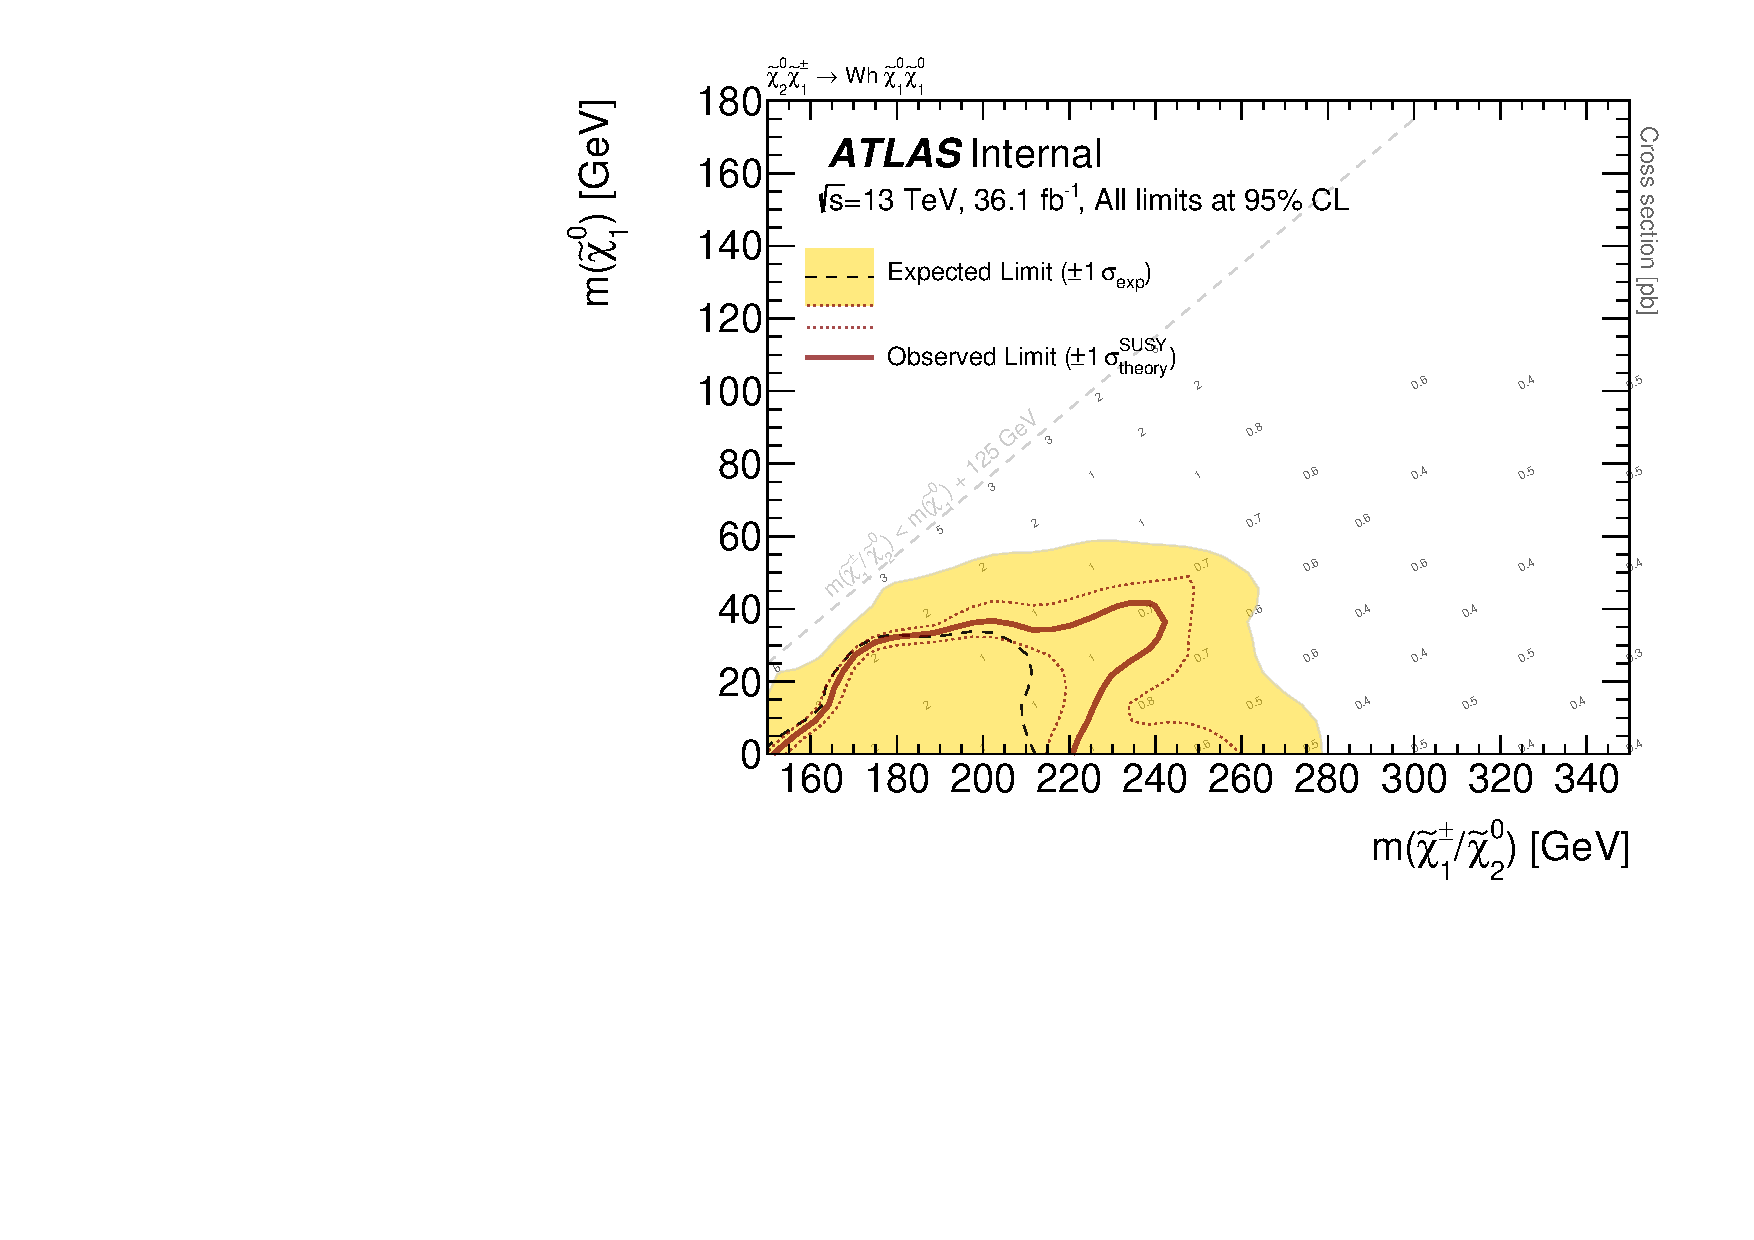
\includegraphics[width=0.5\textwidth]{data/plot/HistFitterResults/contourPlotterWhSS_upperLimit.pdf}
\end{figure}
\end{frame}

\begin{frame}{Results: Exclusion Limits}
\begin{itemize}
\item The exclusion limits for the masses of $\tilde{\chi}_1^\pm$ and $\tilde{\chi}_2^0$ are extended up to 245 GeV, and the exclusion limits for the mass of $\tilde{\chi}_1^0$ are extended up to 40 GeV.
\item This means that the mass points inside the contour line are rejected with 95\% confidence level.
\end{itemize}
\begin{figure}
\centering
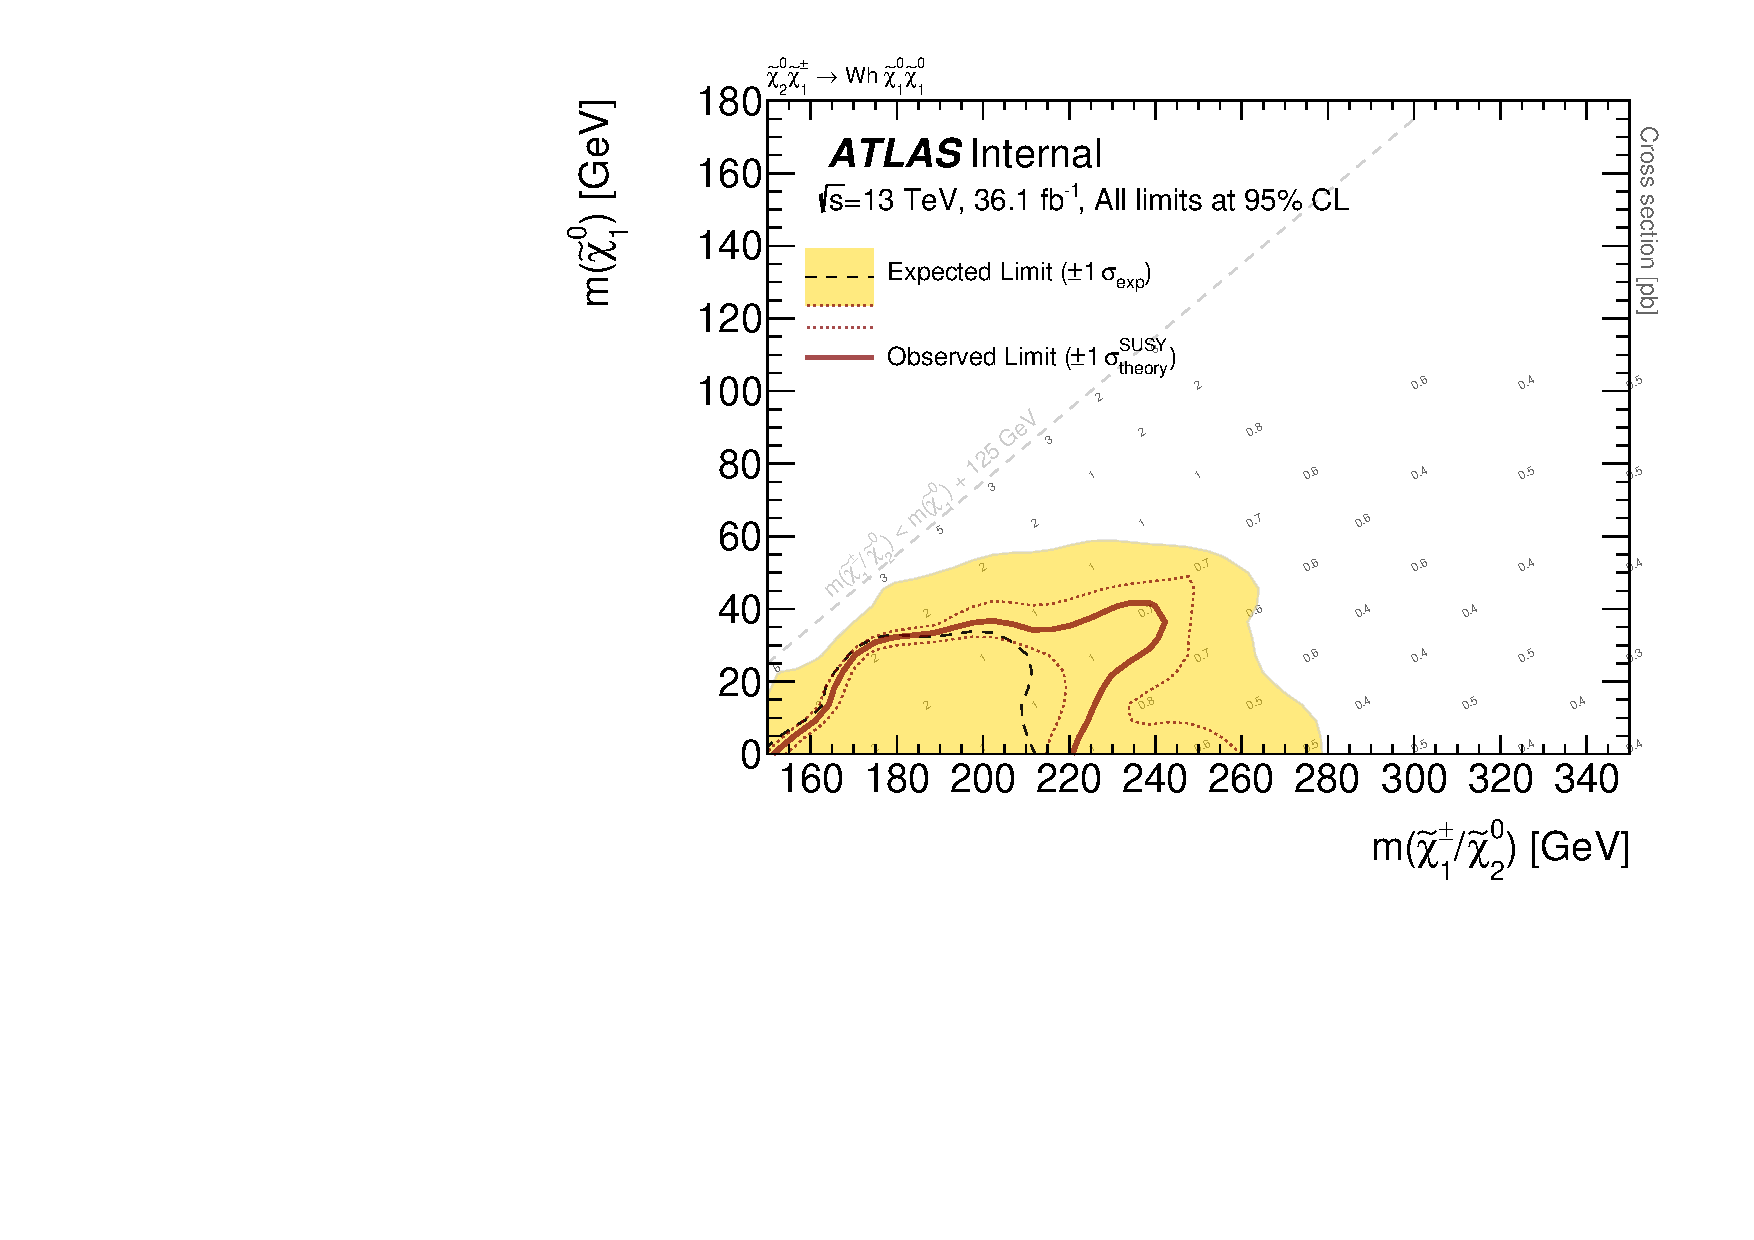
\includegraphics[width=0.5\textwidth]{data/plot/HistFitterResults/contourPlotterWhSS_upperLimit.pdf}
\end{figure}
\end{frame}

\begin{frame}{Conclusion}
\begin{itemize}
\item By using the ATLAS data with total integrated luminosity 36.1 fb$^{-1}$, we searched for the electroweak pair production of a chargino and a neutralino
($p + p \rightarrow \tilde{\chi}_1^\pm + \tilde{\chi}_2^0$), with the Wh channel $\tilde{\chi}_1^\pm \rightarrow \tilde{\chi}_1^0 + W$ and $\tilde{\chi}_2^0 \rightarrow \tilde{\chi}_1^0 + h$, and the same-sign channel.
\item The numbers of observed events in data were consistent with the prediction in the SM.
\item The exclusion limits for the masses of $\tilde{\chi}_1^\pm$ and $\tilde{\chi}_2^0$ are extended up to 245 GeV, and the exclusion limits for the mass of $\tilde{\chi}_1^0$ are extended up to 40 GeV, with 95\% confidence level.
\end{itemize}
\end{frame}

\begin{frame}
\begin{center}
\huge
Thank You
\end{center}
\end{frame}

\section{Backup}
\begin{frame}
\begin{center}
\huge
Backup
\end{center}
\end{frame}

\subsection{Supersymmetry : R-parity}
\begin{frame}{Supersymmetry : R-parity}
\begin{itemize}
\item The baryon number $B$ is defined by $\frac{1}{3} (n_q - n_{\bar{q}})$, where $n_q$ is the number of quarks and $n_{\bar{q}}$ is the number of anti-quarks.
\item The lepton number $L$ is defined by $n_l - n_{\bar{l}}$, where $n_l$ is the number of leptons and $n_{\bar{l}}$ is the number of anti-leptons.
\item In SM, $(B-L)$ is conserved. But in SUSY, it is no longer conserved.
\item To keep $(B-L)$ conservation and prevent the proton decay, the R-parity $P_R$ is introduced.
\begin{equation*}
P_R = (-1)^{3(B-L)-2s}
\end{equation*}
where s is the spin.
\end{itemize}
\end{frame}

\subsection{Charge Flip Background : Likelihood Method}
\begin{frame}
\begin{center}
\huge
Charge Flip Background : Likelihood Method
\end{center}
\end{frame}

\begin{frame}{Likelihood Method : Method}
\begin{itemize}
\item The probability that the charge of an electron is flipped is denoted by the charge-flip rate $\epsilon_i$, where the index i represents the dependency on the $p_T$ and $|\eta|$ of the electron.
\item The value of index i is defined by the index of the following grids in the table.

\begin{table}[htbp]
\centering
\begin{tabular}{|c|c|}
\hline
Variable & Boundary of the bins \\
\hline
$p_T$ (GeV) &  25, 60, 90, 130, 150, 1000 \\
\hline
$|\eta|$ & 0, 0.50, 1.00, 1.37, 1.52, 1.80, 2.00, 2.47 \\
\hline
\end{tabular}
\caption{Binning in $p_T$ and $|\eta|$ for the charge-flip rate $\epsilon_i$.}
\end{table}

\item The probability $p_{ij}$ that an OS data event becomes a SS data event (with the leading lepton in bin $i$ and the subleading lepton in bin $j$) is
\begin{equation*}
p_{ij} = (1 - \epsilon_i)\epsilon_j + (1 - \epsilon_j)\epsilon_i
\end{equation*}
\end{itemize}

\end{frame}

\begin{frame}{Likelihood Method : Definition of Control Region}
A control region is defined.
\begin{itemize}
\item Trigger requirement
\item exactly 2 signal leptons
\item 2 electrons
\item $25 <p_T < 1000$
\item $|\eta| < 2.47$
\end{itemize}
\end{frame}

\begin{frame}{Likelihood Method : Method}
\begin{itemize}
\item The charge flip rate $\epsilon_i$ is measured by using the data in the control region, within the Z mass window cut of 80-100 GeV.
\item The events inside the Z mass window is then subtracted by the non-Zee processes, by using the sideband technique.
\item After the subtraction, the total number of event is denoted by $N^{ij}$, and the number of events with two same-sign leptons is denoted by $N^{ij}_{SS}$.
\item The expected value of $N^{ij}_{SS}$ is then given by $\lambda = N^{ij}p_{ij}$. And, if $N^{ij}_{SS}$ is described by a Poisson distribution, then
\end{itemize}
\begin{equation*}
P(N^{ij}_{SS} | N^{ij}, \epsilon_i, \epsilon_j) = \frac{(N^{ij}p_{ij})^{N^{ij}_{SS}} e^{-N^{ij}p_{ij}}}{N^{ij}_{SS}!}
\end{equation*}
\end{frame}

\begin{frame}{Likelihood Method : Method}
\begin{itemize}
\item Converting it to the likelihood function L and taking the negative natural log yields
\end{itemize}
\begin{equation*}
\begin{split}
-\ln L &= -\ln\prod_{ij} P(N^{ij}_{SS} | N^{ij}, \epsilon_i, \epsilon_j) \\
&= - \sum_{ij} \Big[ N^{ij}_{SS} \ln (N^{ij}[\epsilon_i (1-\epsilon_j) + (1-\epsilon_i) \epsilon_j]) \\
&- N^{ij}[\epsilon_i (1-\epsilon_j) + (1-\epsilon_i) \epsilon_j] \Big] + \text{constant}
\end{split}
\end{equation*}
\begin{itemize}
\item where the summation over $i$ and $j$ is taken over all $p_T$ and $|\eta|$ bins of both electrons.
\item By minimizing this likelihood, the charge-flip rate can be estimated.
\end{itemize}
\end{frame}

\begin{frame}{Likelihood Method : Background Subtraction}
Both for data and MC
\begin{itemize}
\item Central region: 80 - 100 GeV
\item Sideband region: 60 - 80 and 100 - 120 \\
(Sideband width 20 GeV)
\end{itemize}
\begin{equation*}
N_{Central} = N_{Central} - \frac{20}{20+20} N_{SB}
\end{equation*}
\begin{itemize}
\item Background subtraction is done both on $N^{ij}$ and $N^{ij}_{SS}$
\end{itemize}
\end{frame}

\begin{frame}{Likelihood Method : Result for Charge Flip Rate (statistical error only)}
\begin{itemize}
\item Results by likelihood method from data, $\epsilon_{\text{lik,data}}$
\item The error is statistical only, from likelihood method, $\sigma_{\text{lik,data}}$.
\end{itemize}
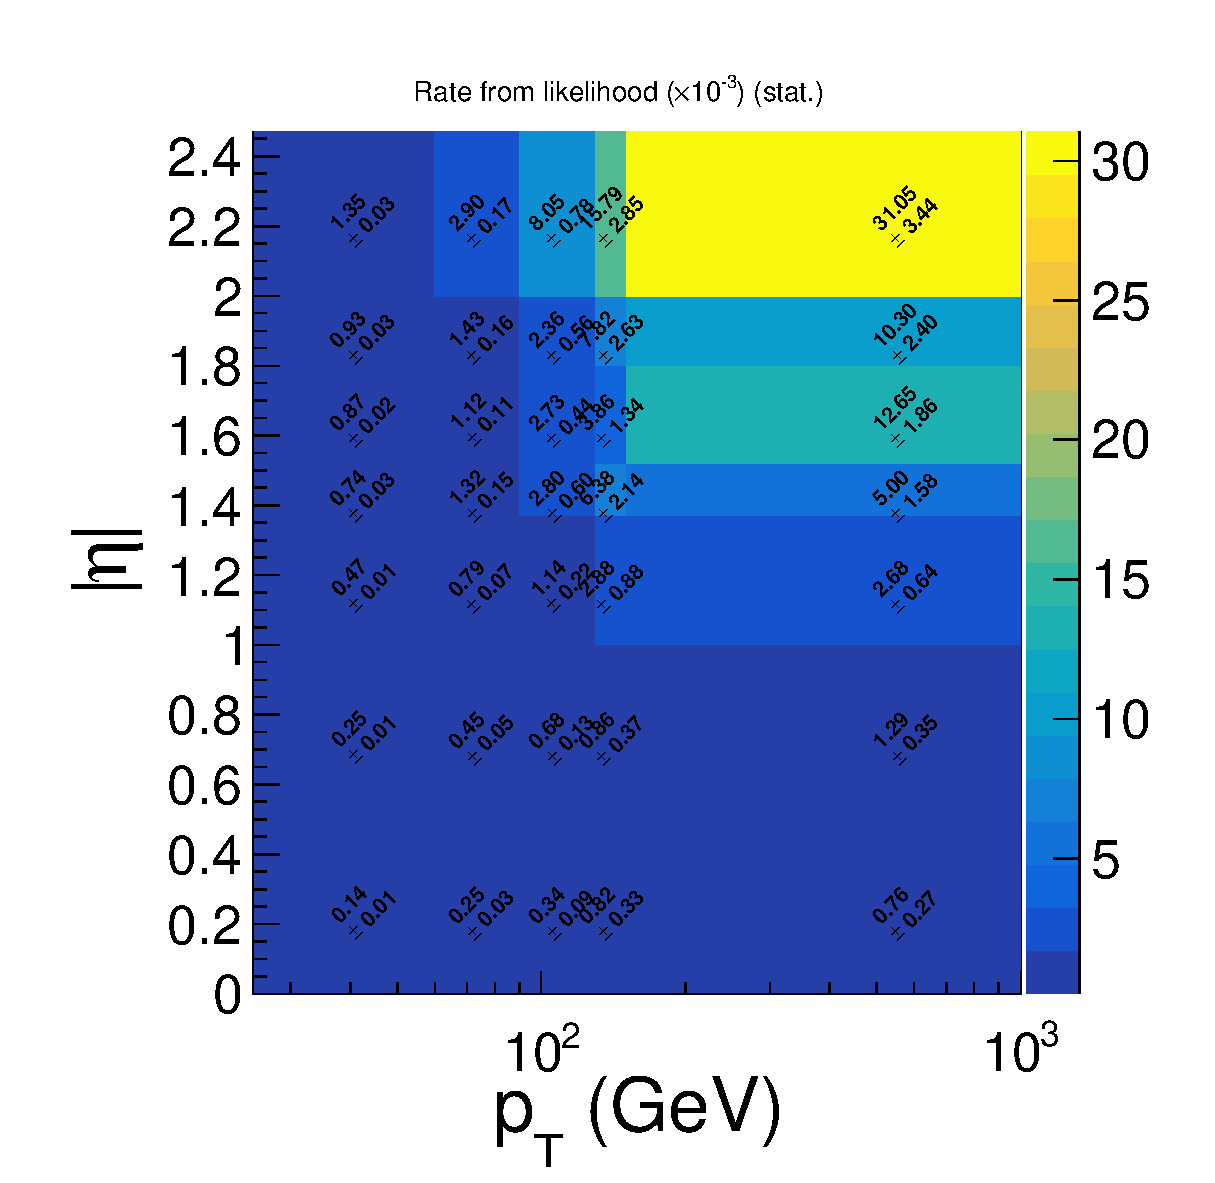
\includegraphics[width=0.6\textwidth]{data/plot/charge_flip/FitPlots/data_cf_rate_stat.eps}
\end{frame}

\begin{frame}{Likelihood Method : MC Truth Validation}
\begin{itemize}
\item Results by likelihood method from MC (blue points)
\item Results by MC truth (red points)
\end{itemize}
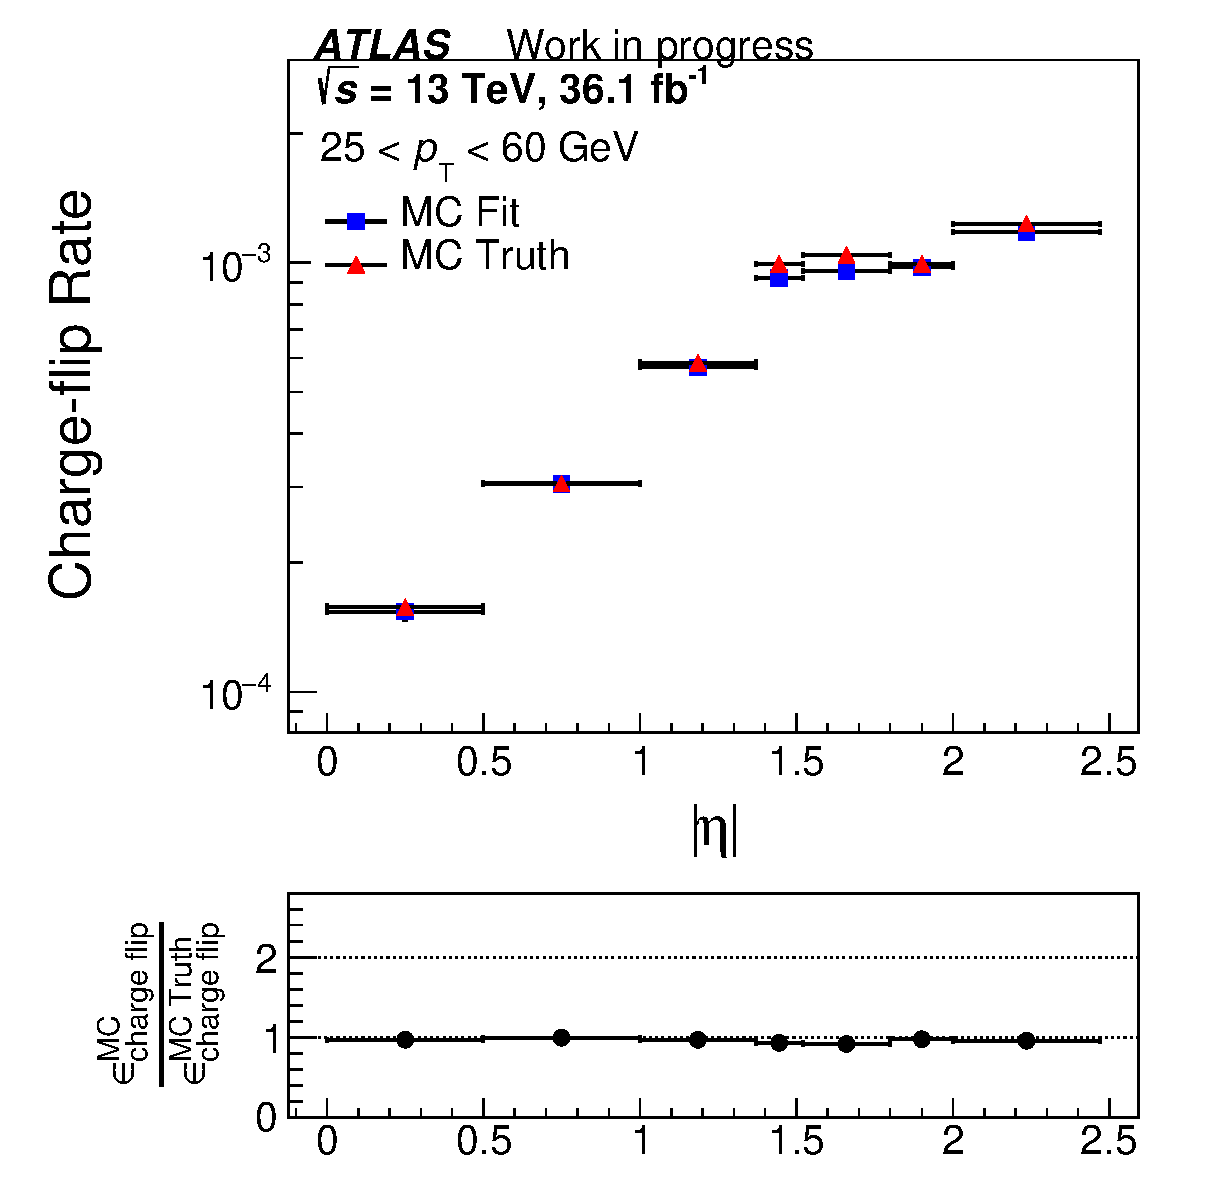
\includegraphics[width=0.3\textwidth]{data/plot/charge_flip/FitPlots/mc_cf_rate_0.eps}
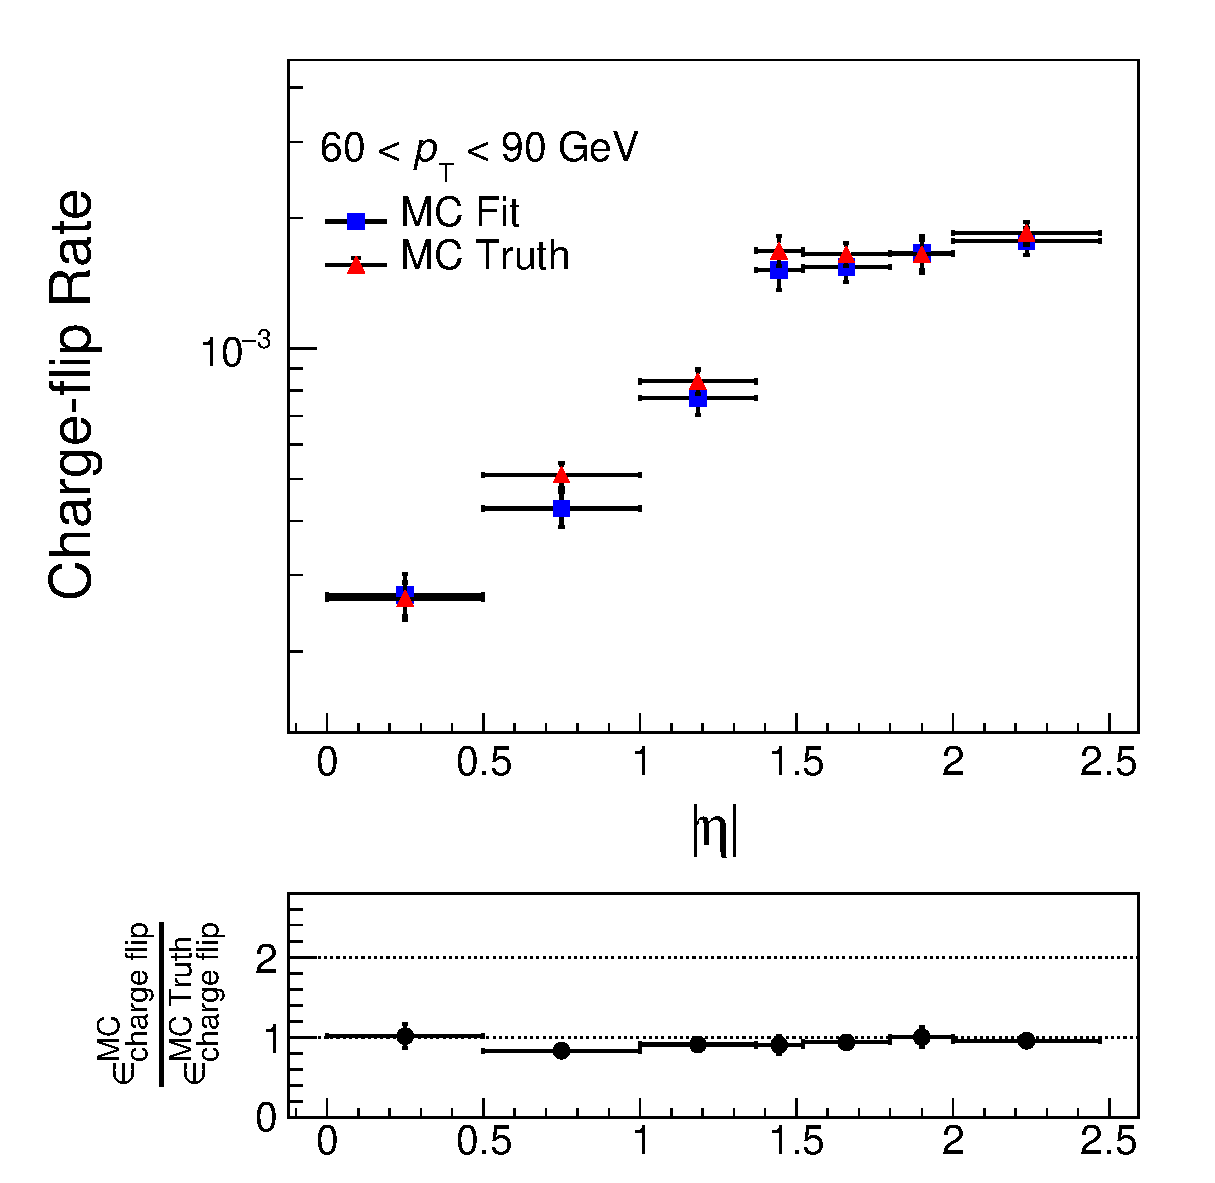
\includegraphics[width=0.3\textwidth]{data/plot/charge_flip/FitPlots/mc_cf_rate_1.eps}
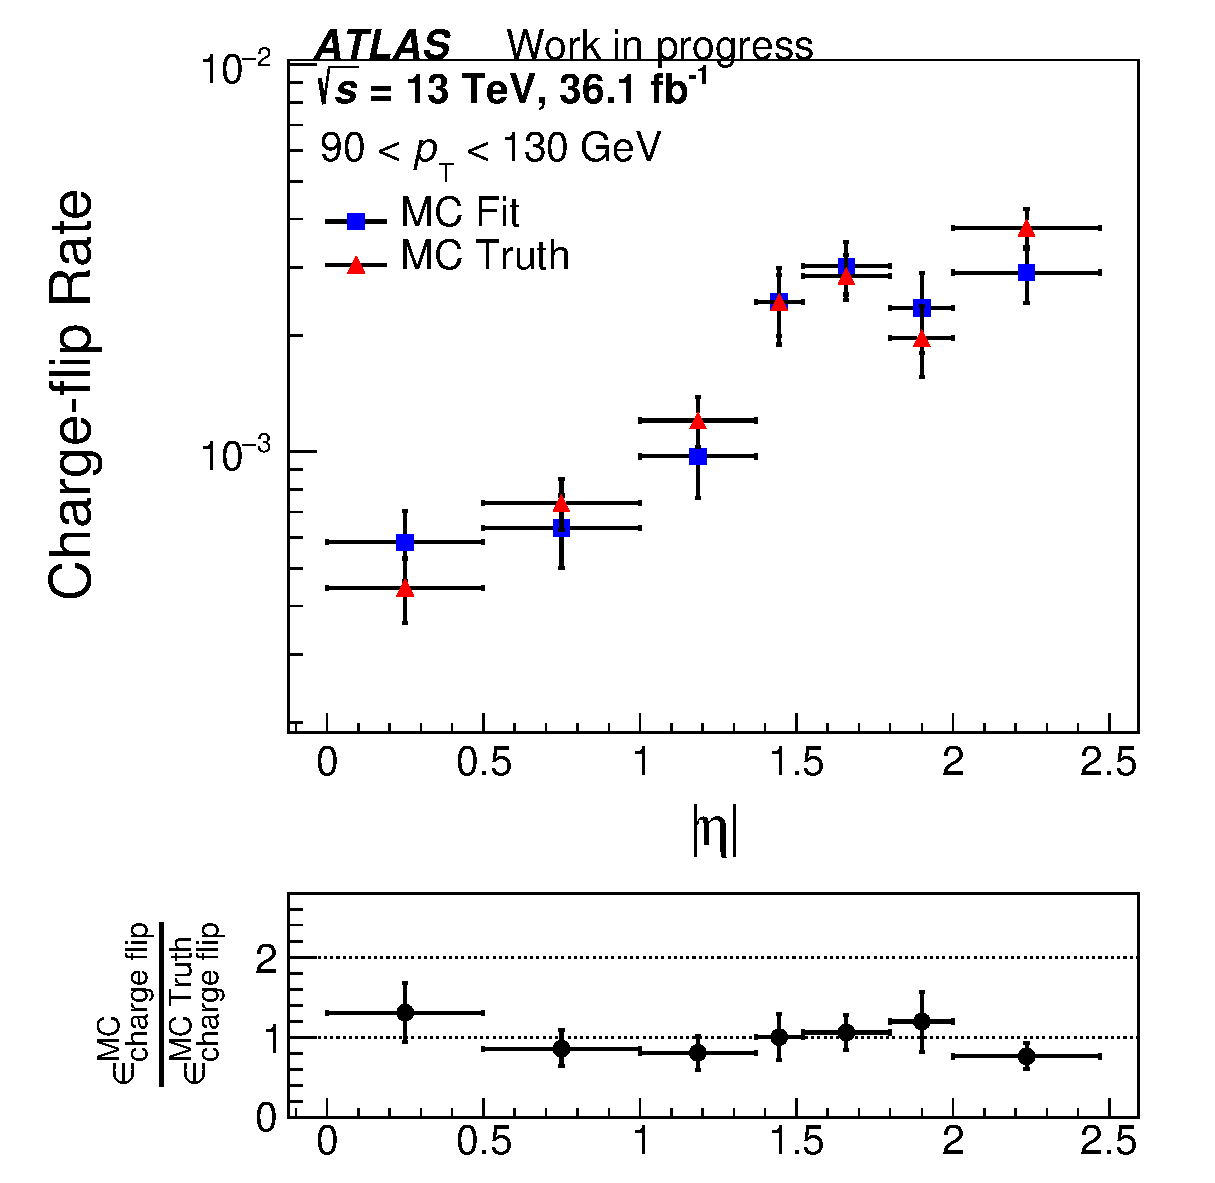
\includegraphics[width=0.3\textwidth]{data/plot/charge_flip/FitPlots/mc_cf_rate_2.eps} \\
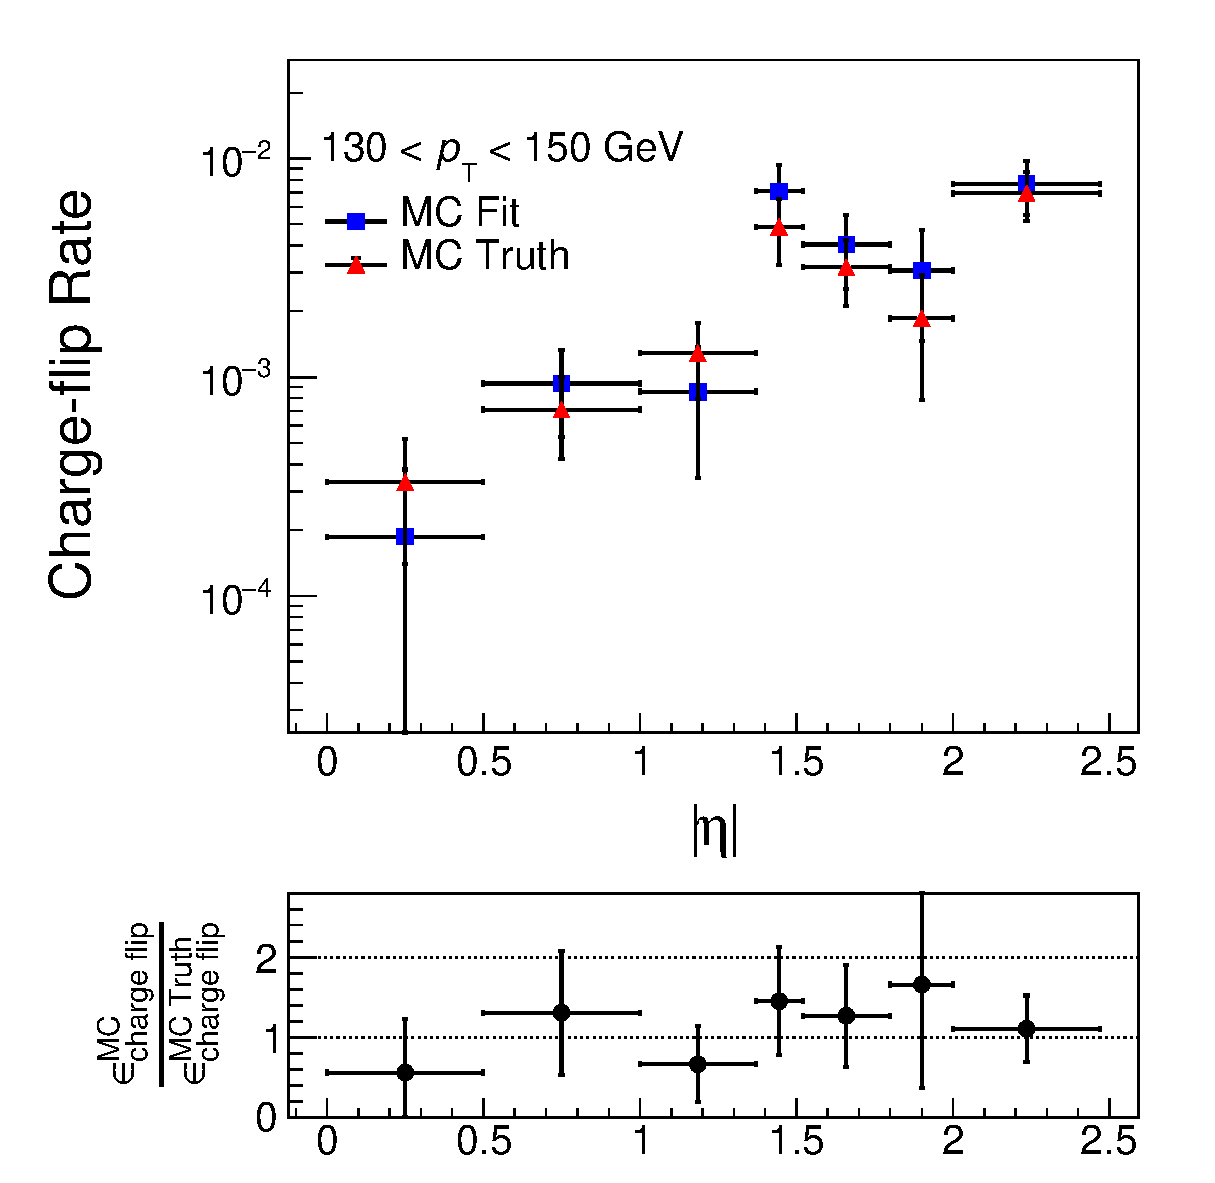
\includegraphics[width=0.3\textwidth]{data/plot/charge_flip/FitPlots/mc_cf_rate_3.eps}
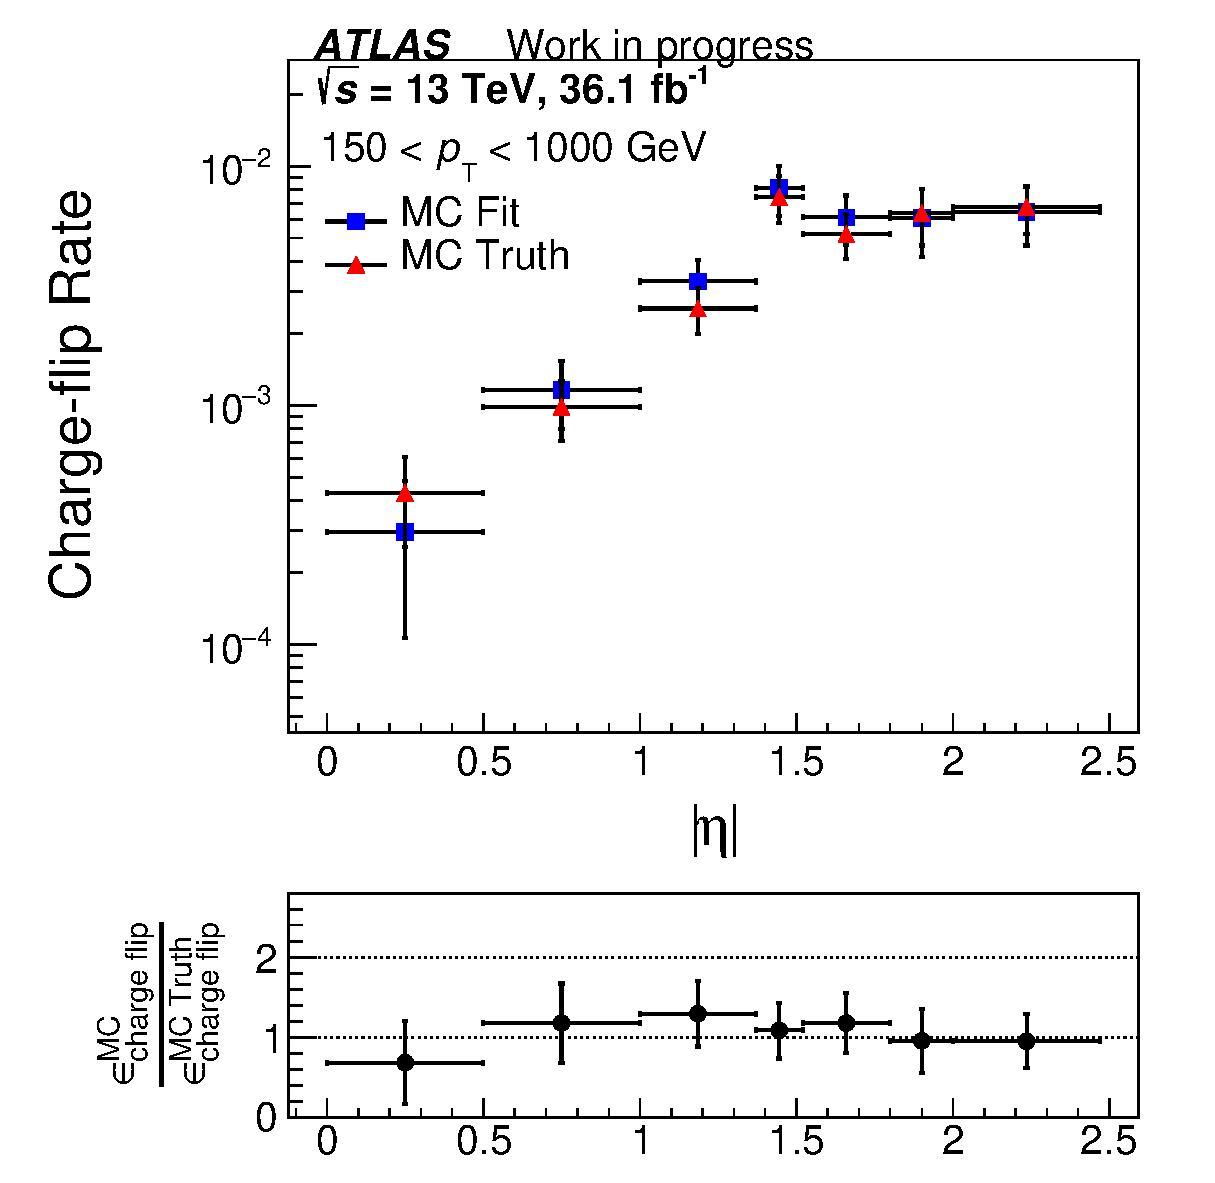
\includegraphics[width=0.3\textwidth]{data/plot/charge_flip/FitPlots/mc_cf_rate_4.eps}
\end{frame}

\begin{frame}{Likelihood Method : MC Truth Matching}
\begin{itemize}
\item It is a complicated part, because we do not know the original charge of the reconstructed electron for some cases.
\item The reconstructed electrons match the truth particle by the smallest $\Delta R$ ($\Delta R < 0.1$).
\item No match for reconstructed electrons if no any truth particle is inside $\Delta R < 0.1$. (cannot find the original charge)
\item If the truth particle is matched, the truth particle is not electron. (fake lepton, not charge flip)
\end{itemize}
\end{frame}

\begin{frame}{Likelihood Method : MC Truth Matching}
\begin{itemize}
\item If the truth particle is electron, the (grand)mother particle is not Z Boson. (ignore it)
\item If (grand)mother particle is Z Boson, the daughter of the Z Boson is not electron.  (ignore it)
\item If the daughter of the Z Boson is electron, the charge of that electron is the original charge.
\end{itemize}
\centering
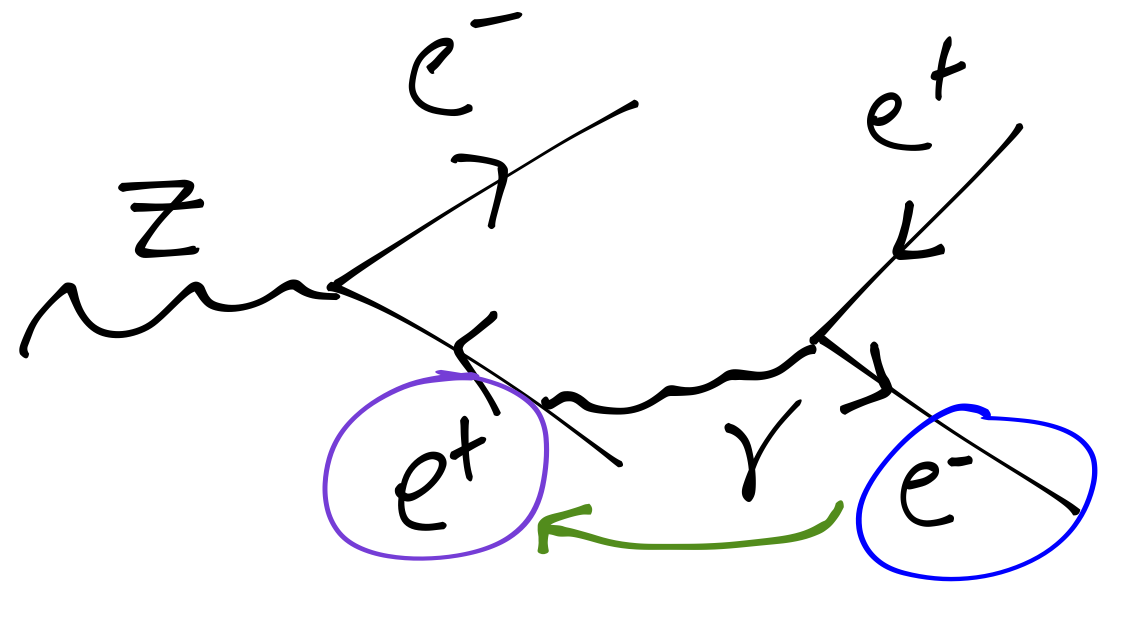
\includegraphics[width=0.5\textwidth]{data/photo/charge_flip/MC-truth.png}
\end{frame}

\begin{frame}{Likelihood Method : Systematic uncertainties due to likelihood method}
For each bin, the systematic uncertainties due to likelihood method are estimated by the difference between the likelihood method and the MC truth method.

For MC,
\begin{equation*}
\sigma_{\text{truth,MC}} = | \epsilon_{\text{lik,MC}} - \epsilon_{\text{MC truth}} |
\end{equation*}
For data,
\begin{equation*}
\sigma_{\text{truth,data}} = \epsilon_{\text{lik,data}} \times \frac{\sigma_{\text{truth,MC}}}{\epsilon_{\text{lik,MC}}}
\end{equation*}
\end{frame}

\begin{frame}{Likelihood Method : Systematic uncertainties due to background substraction}
Nominal:
\begin{itemize}
\item Central region: 80 - 100 GeV, Sideband width: 20 GeV
\end{itemize}
Variations:
\begin{itemize}
\item Central region: 80 - 100 GeV, Sideband width: 15 GeV
\item Central region: 80 - 100 GeV, Sideband width: 25 GeV
\item Central region: 75 - 105 GeV, Sideband width: 20 GeV
\item Central region: 80 - 100 GeV, no background subtraction
\end{itemize}
For each bin, the largest deviation from the nominal among these variations is the systematic uncertainty due to background substraction.
\begin{equation*}
\sigma_{\text{bgk}} = max\{| \sigma_{\text{nominal}} - \sigma_{\text{variation}} |\}
\end{equation*}
\end{frame}

\begin{frame}{Likelihood Method : Result for different variation}
\begin{itemize}
\item Results for different variations
\end{itemize}
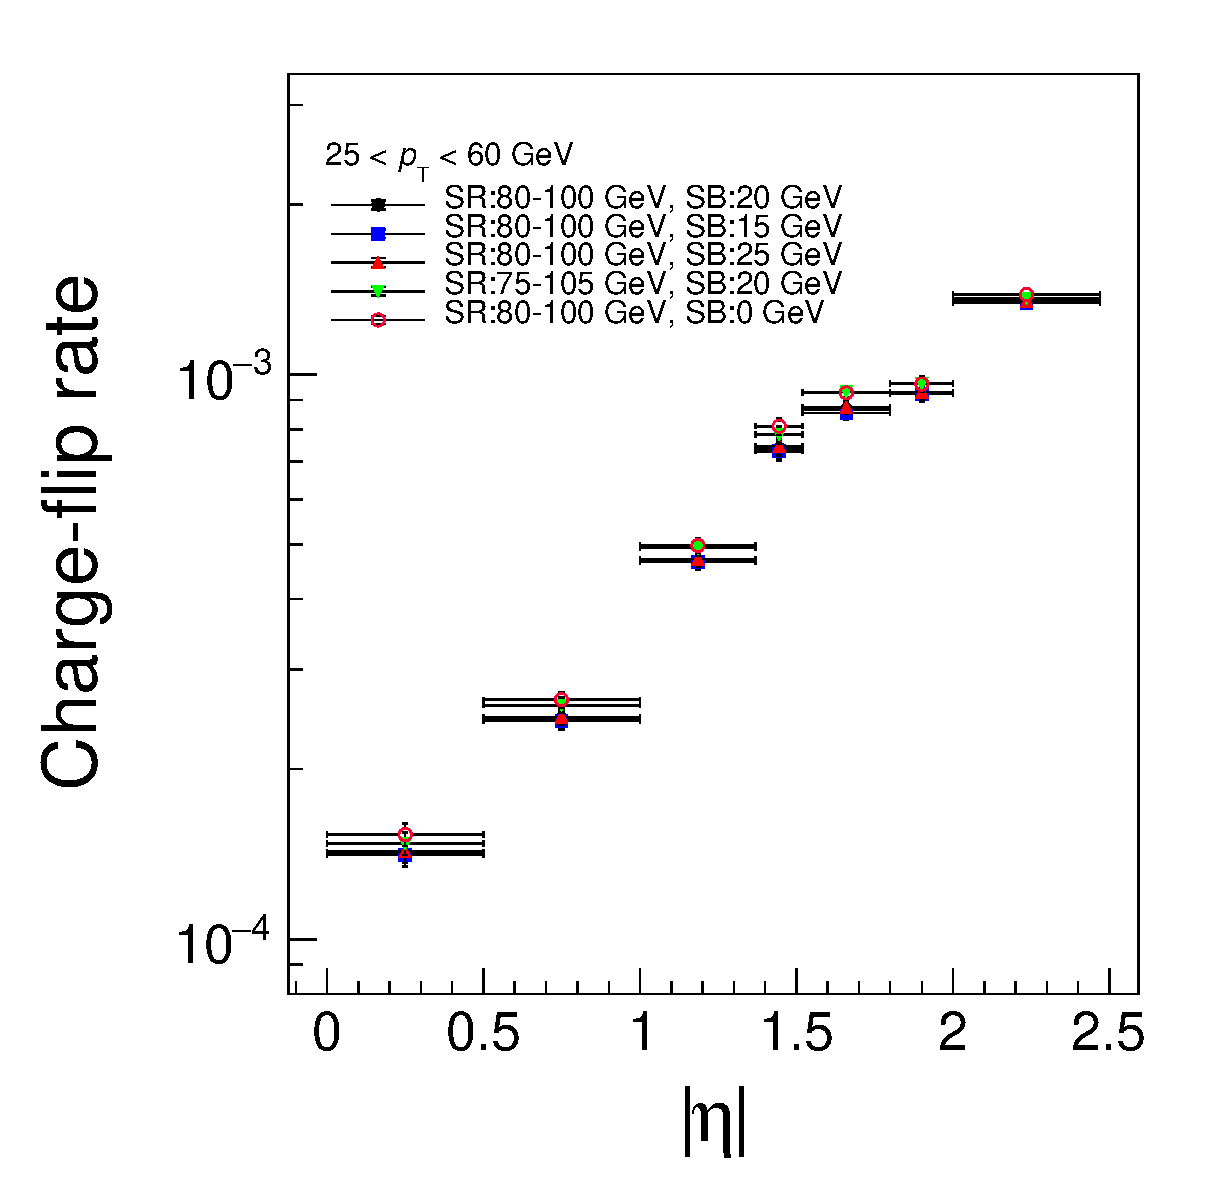
\includegraphics[width=0.3\textwidth]{data/plot/charge_flip/FitPlots/data_cf_comparison_0.eps}
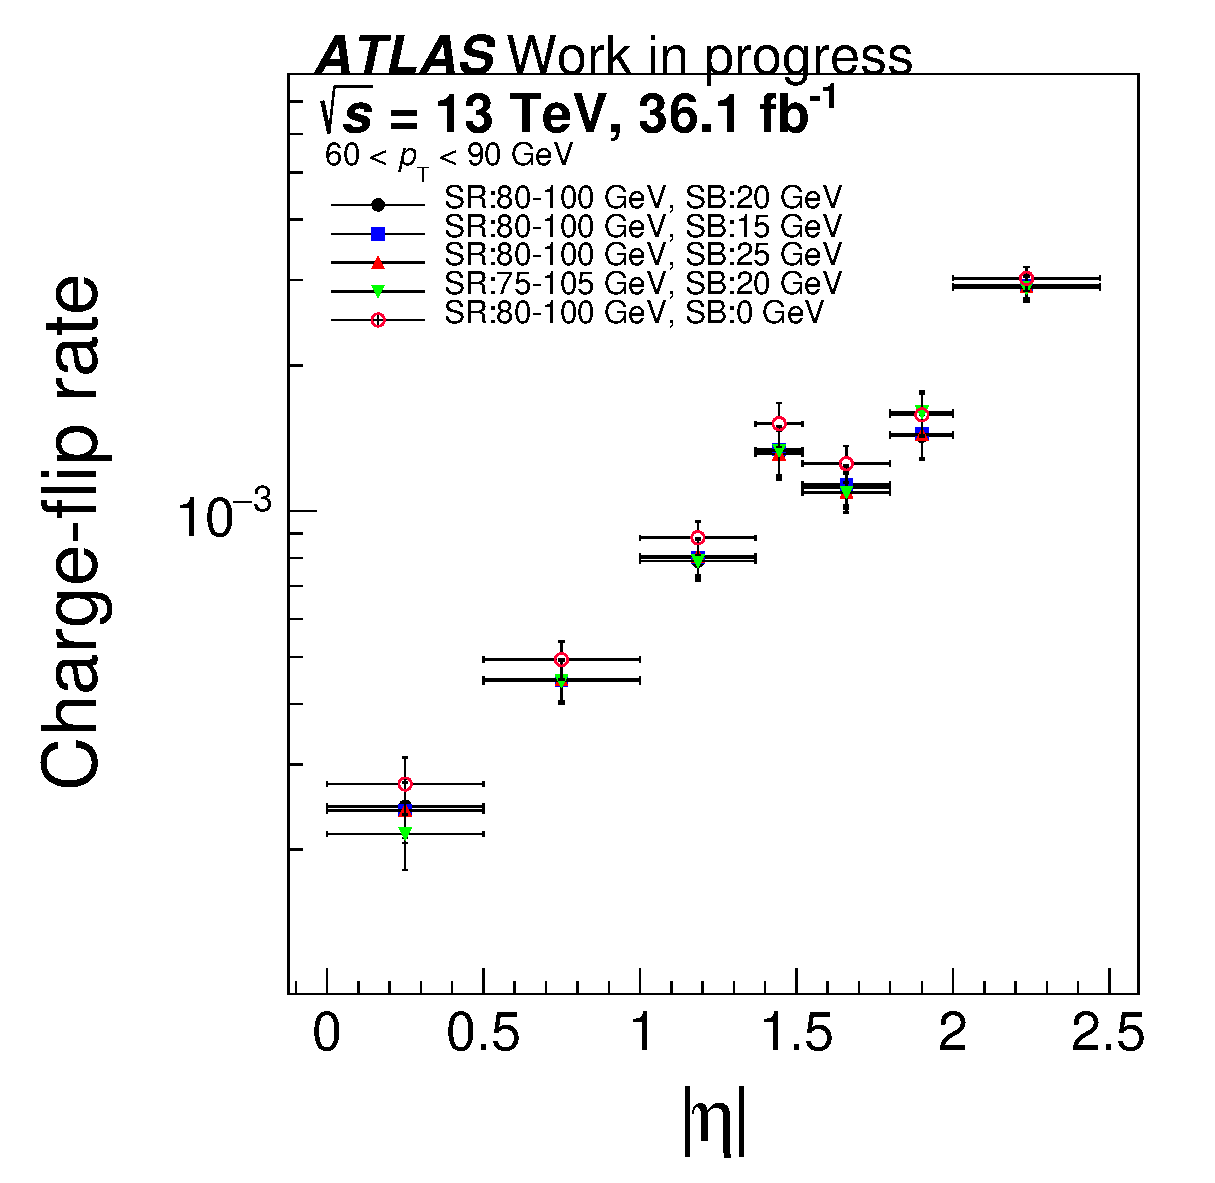
\includegraphics[width=0.3\textwidth]{data/plot/charge_flip/FitPlots/data_cf_comparison_1.eps}
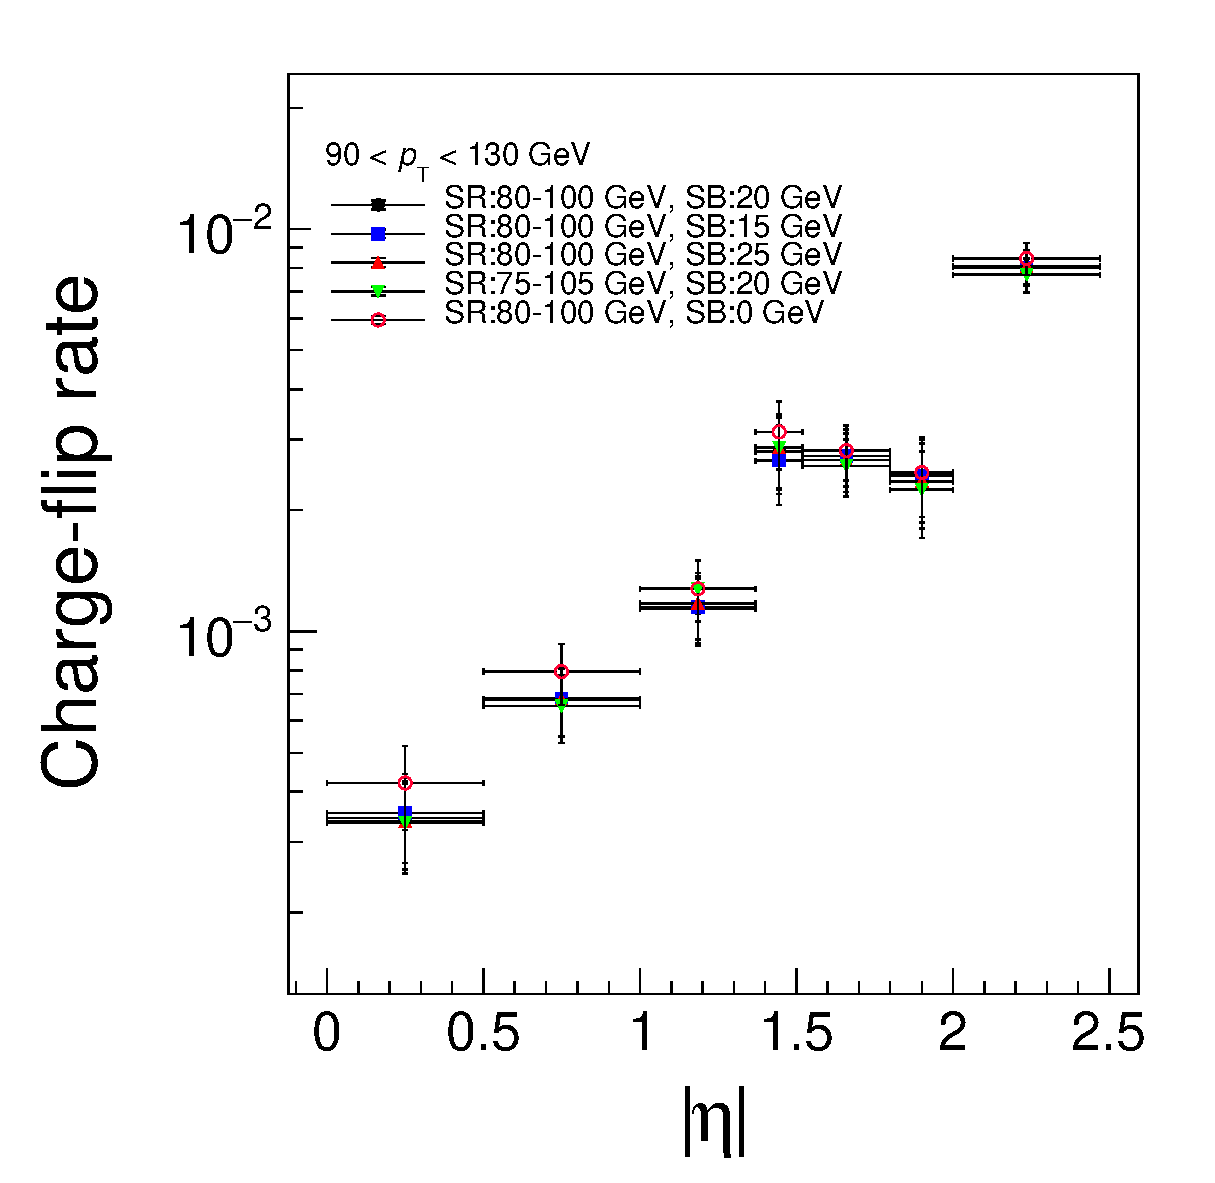
\includegraphics[width=0.3\textwidth]{data/plot/charge_flip/FitPlots/data_cf_comparison_2.eps} \\
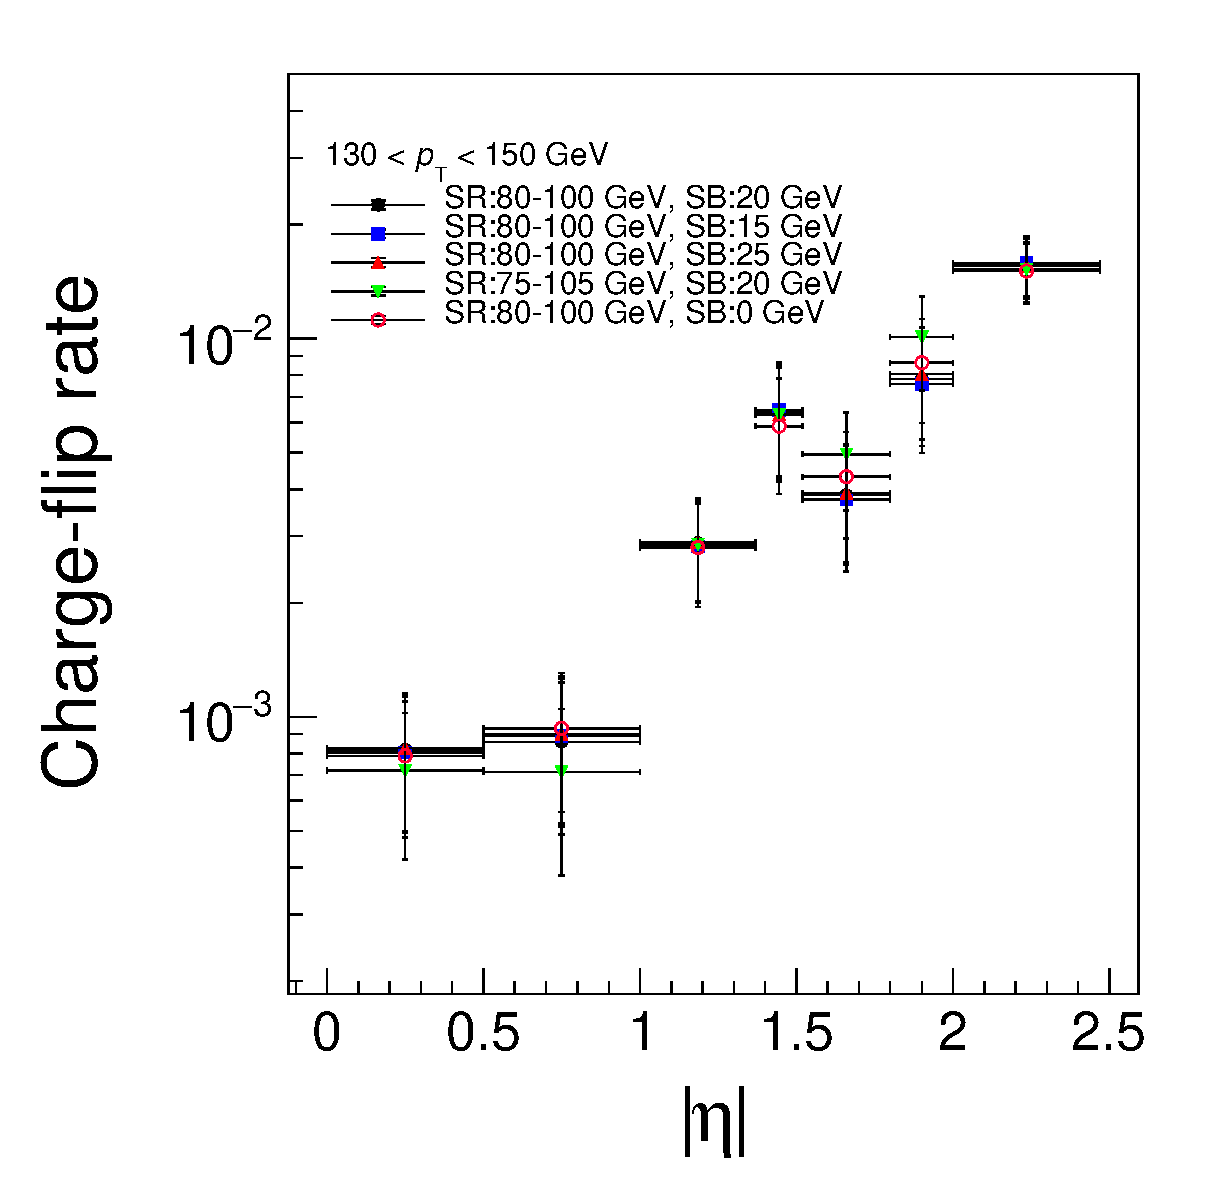
\includegraphics[width=0.3\textwidth]{data/plot/charge_flip/FitPlots/data_cf_comparison_3.eps}
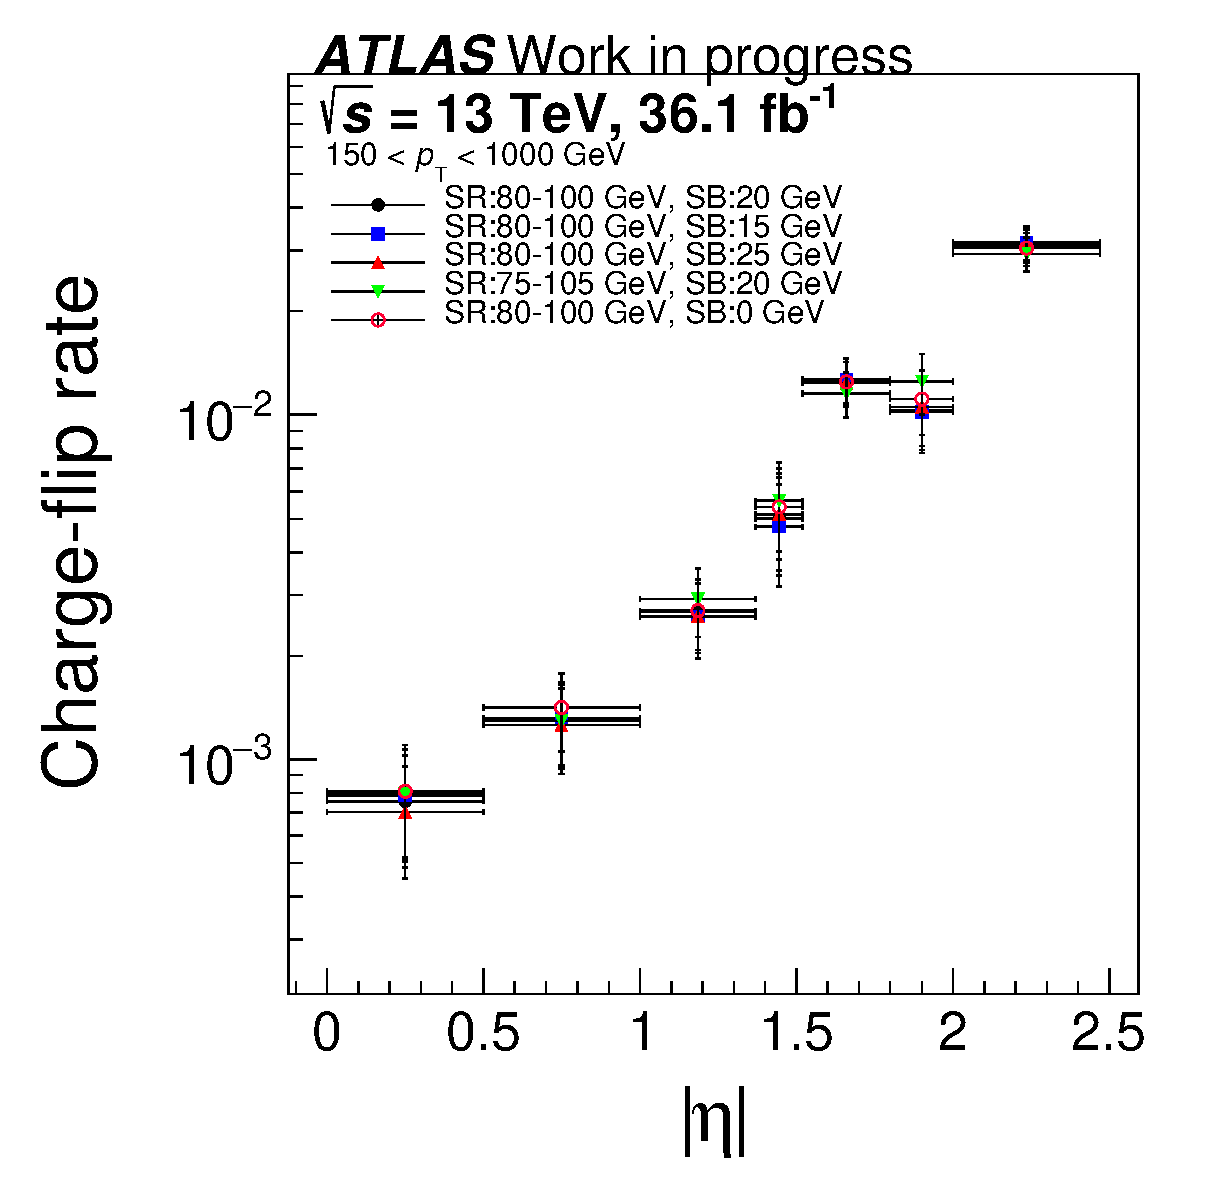
\includegraphics[width=0.3\textwidth]{data/plot/charge_flip/FitPlots/data_cf_comparison_4.eps}
\end{frame}

\begin{frame}{Likelihood Method : Total uncertainties}
\begin{equation*}
\sigma_{\text{sys}} = \sqrt{\sigma_{\text{truth}} ^2 + \sigma_{\text{bgk}} ^2}
\end{equation*}
\begin{equation*}
\sigma_{\text{tot}} = \sqrt{\sigma_{\text{lik}} ^2 + \sigma_{\text{sys}} ^2}
\end{equation*}
\end{frame}

\begin{frame}{Likelihood Method : MC Validation Plots}
\begin{figure}
\centering
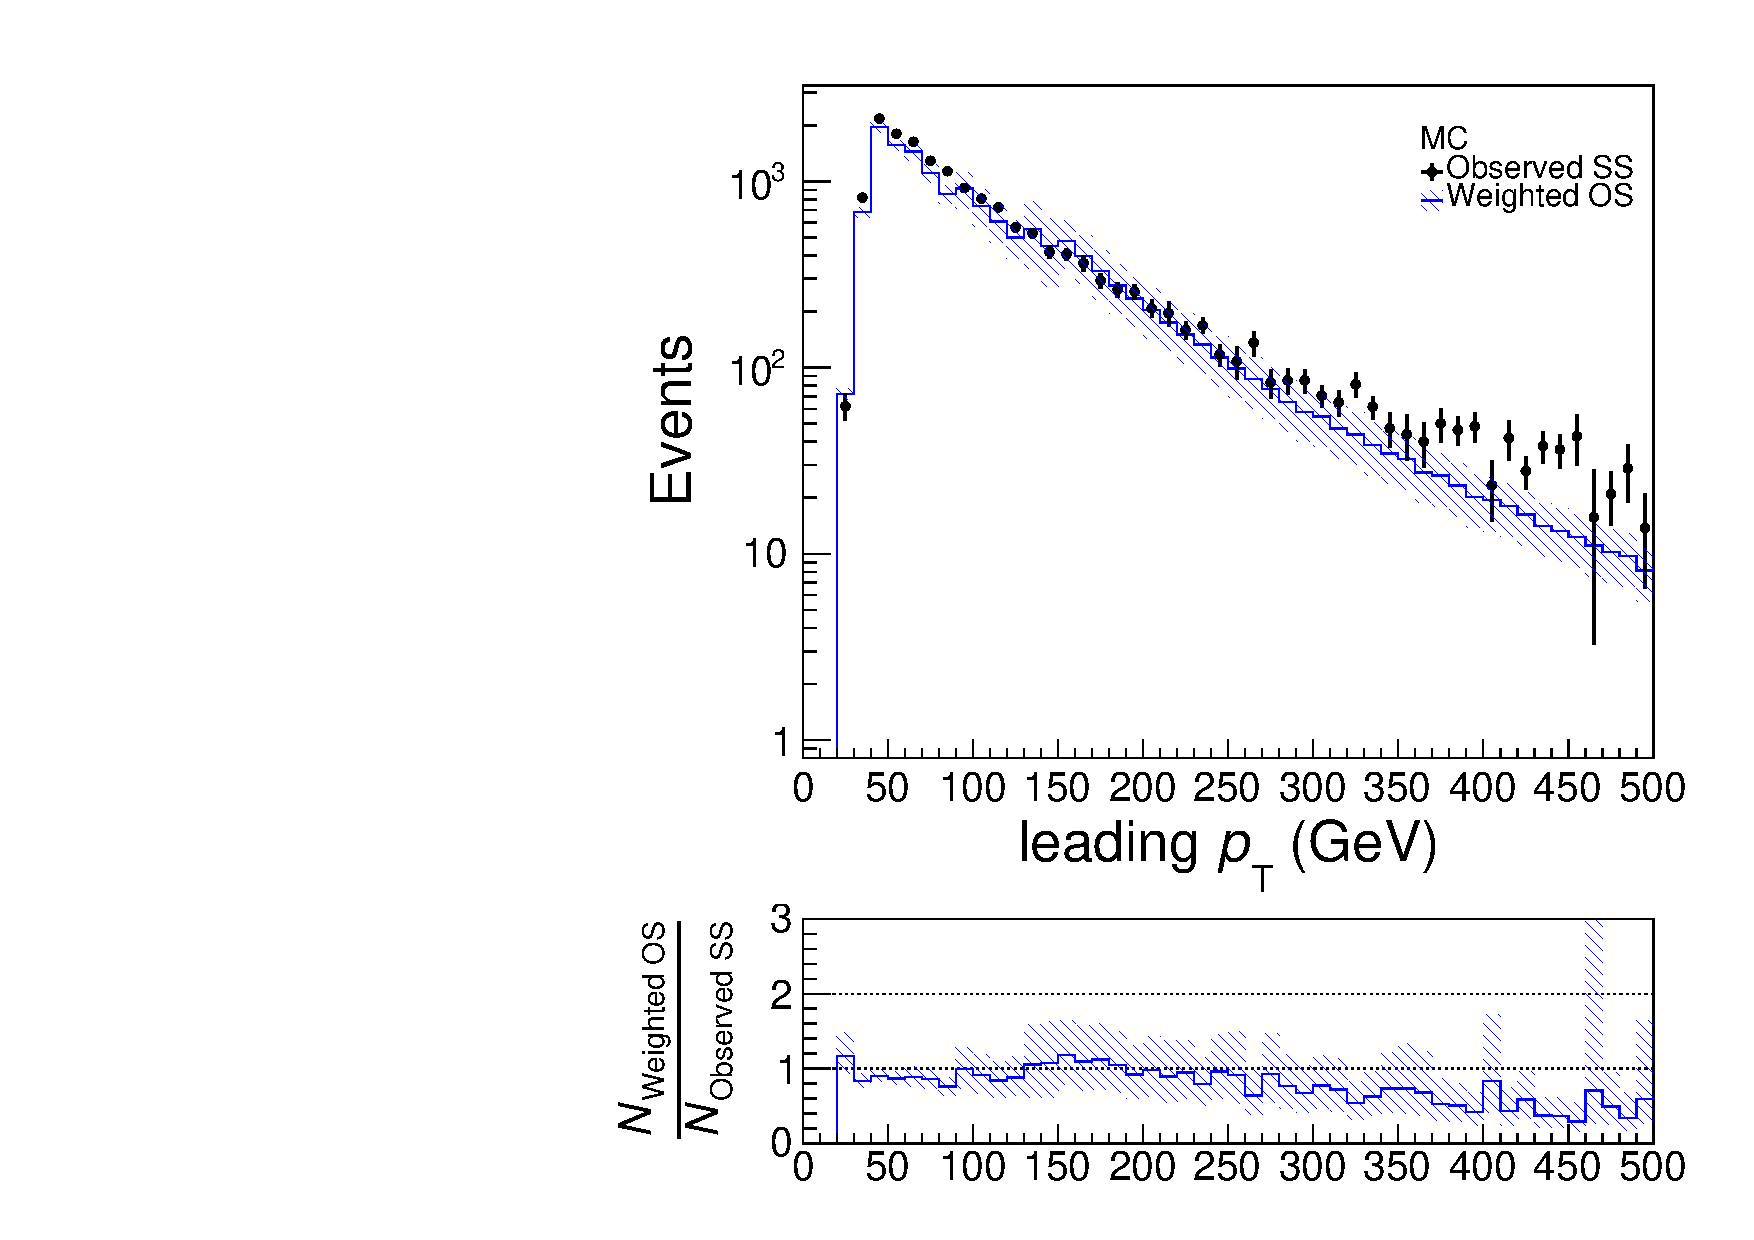
\includegraphics[width=0.3\textwidth]{data/plot/charge_flip/ReweightPlots/plots_NOchfSF/mc_pt_1.pdf}
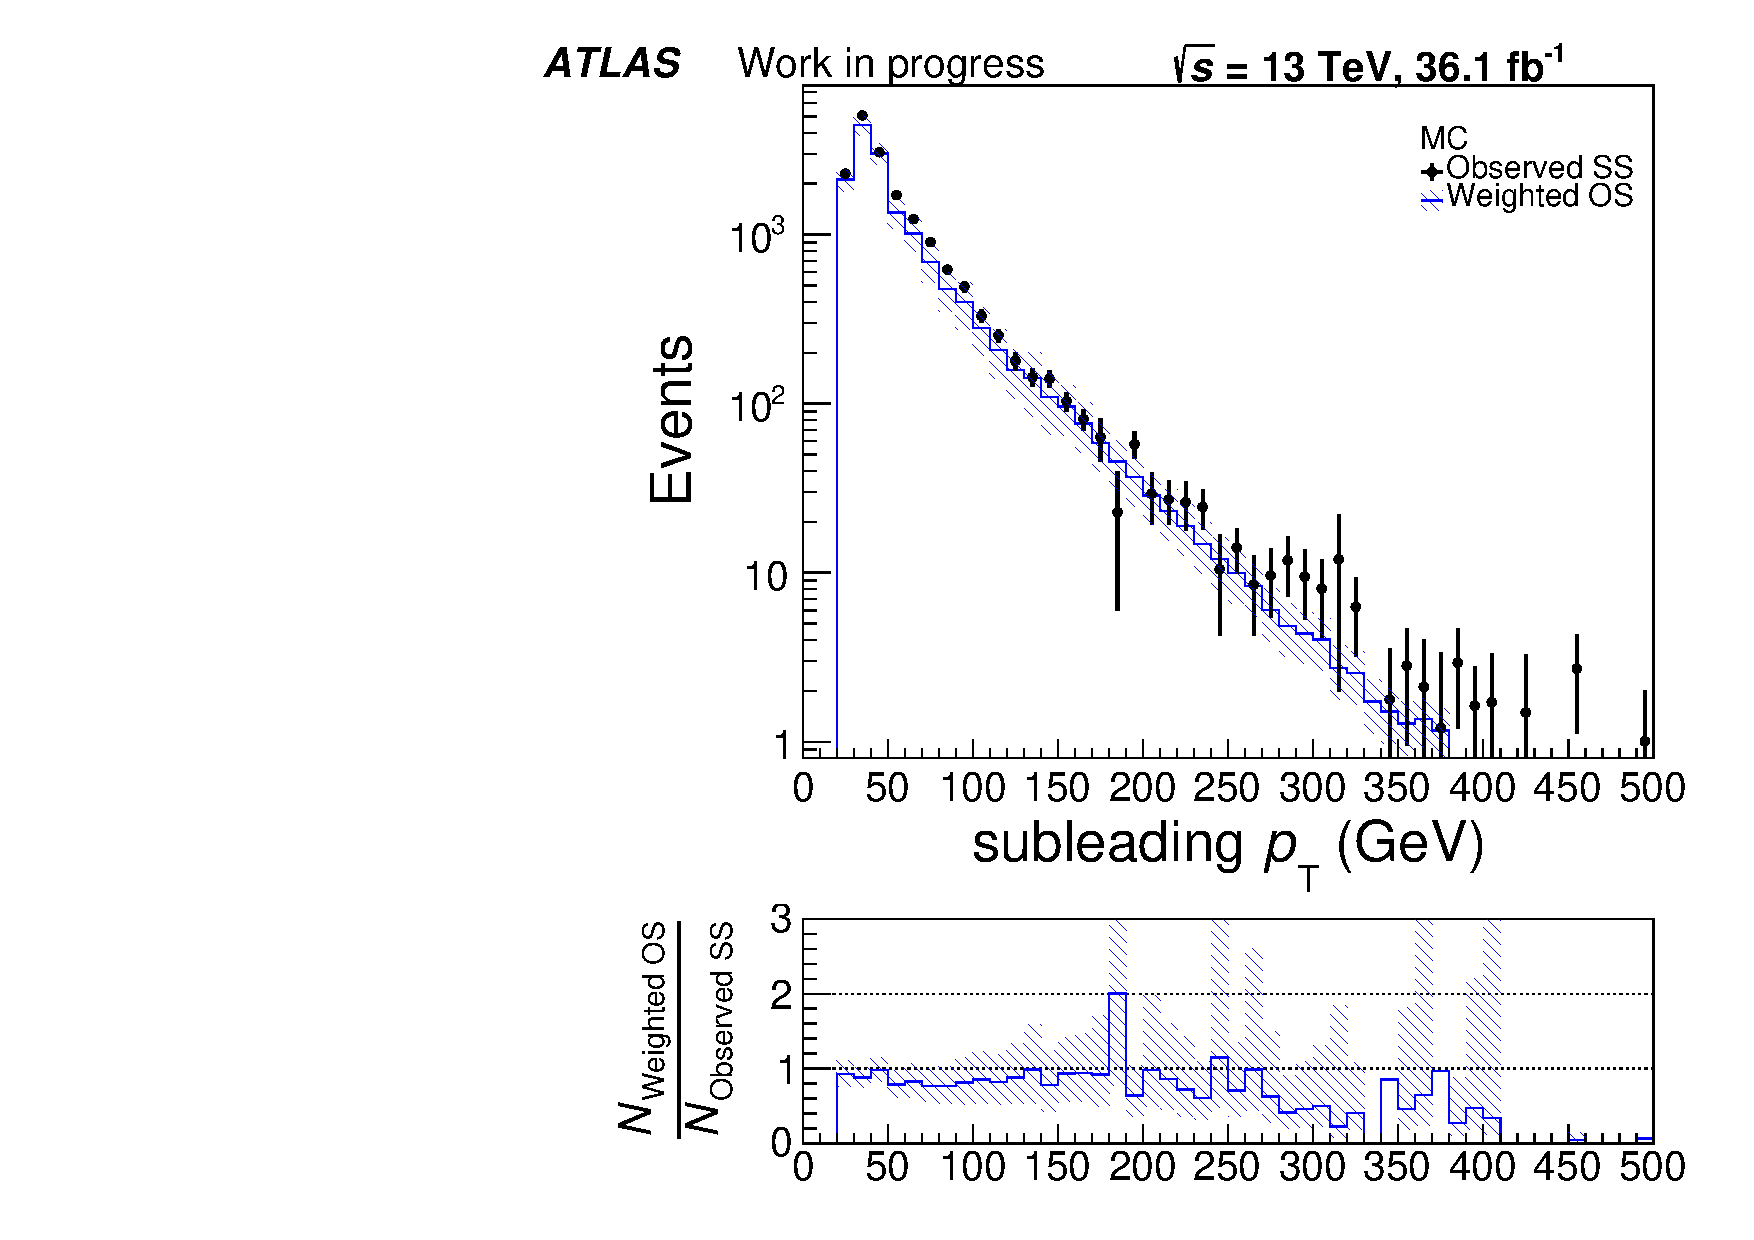
\includegraphics[width=0.3\textwidth]{data/plot/charge_flip/ReweightPlots/plots_NOchfSF/mc_pt_2.pdf} \\
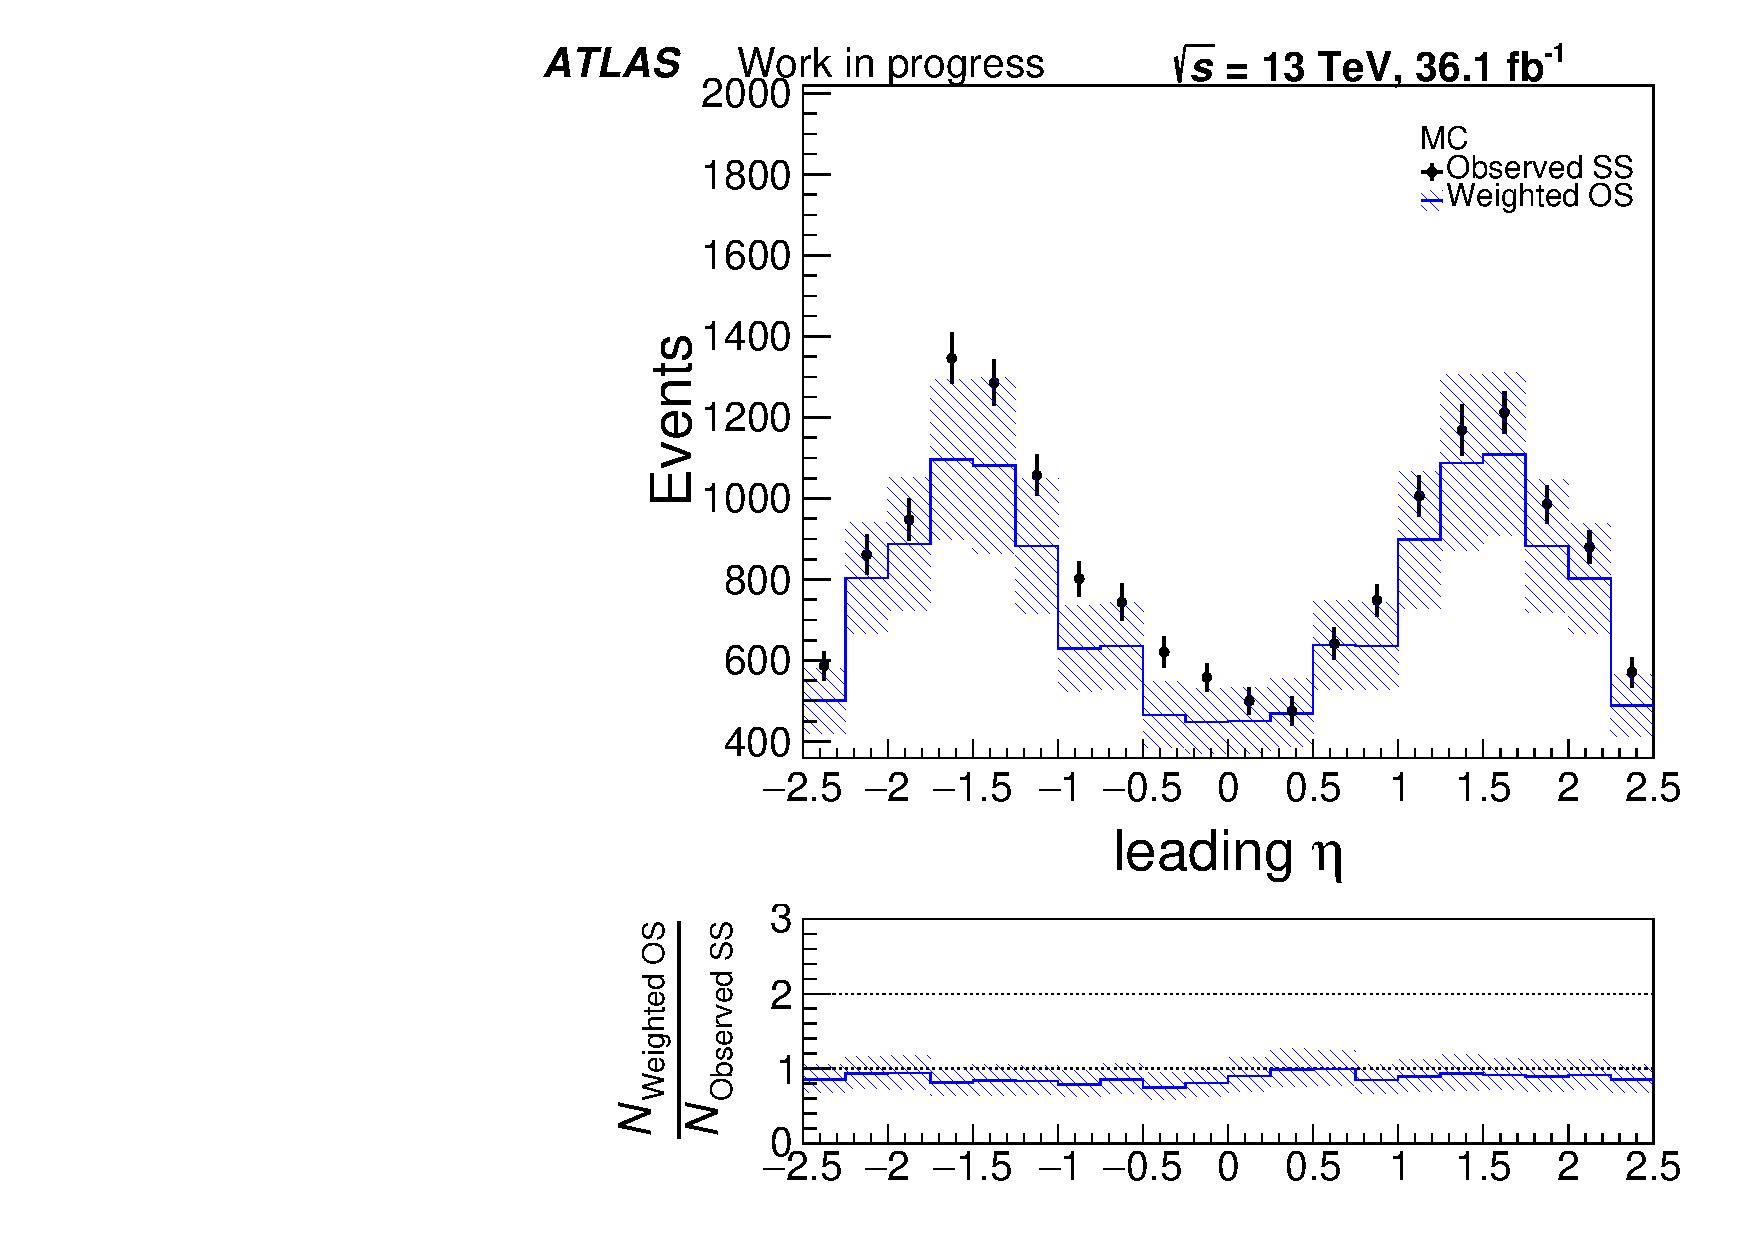
\includegraphics[width=0.3\textwidth]{data/plot/charge_flip/ReweightPlots/plots_NOchfSF/mc_eta_1.pdf}
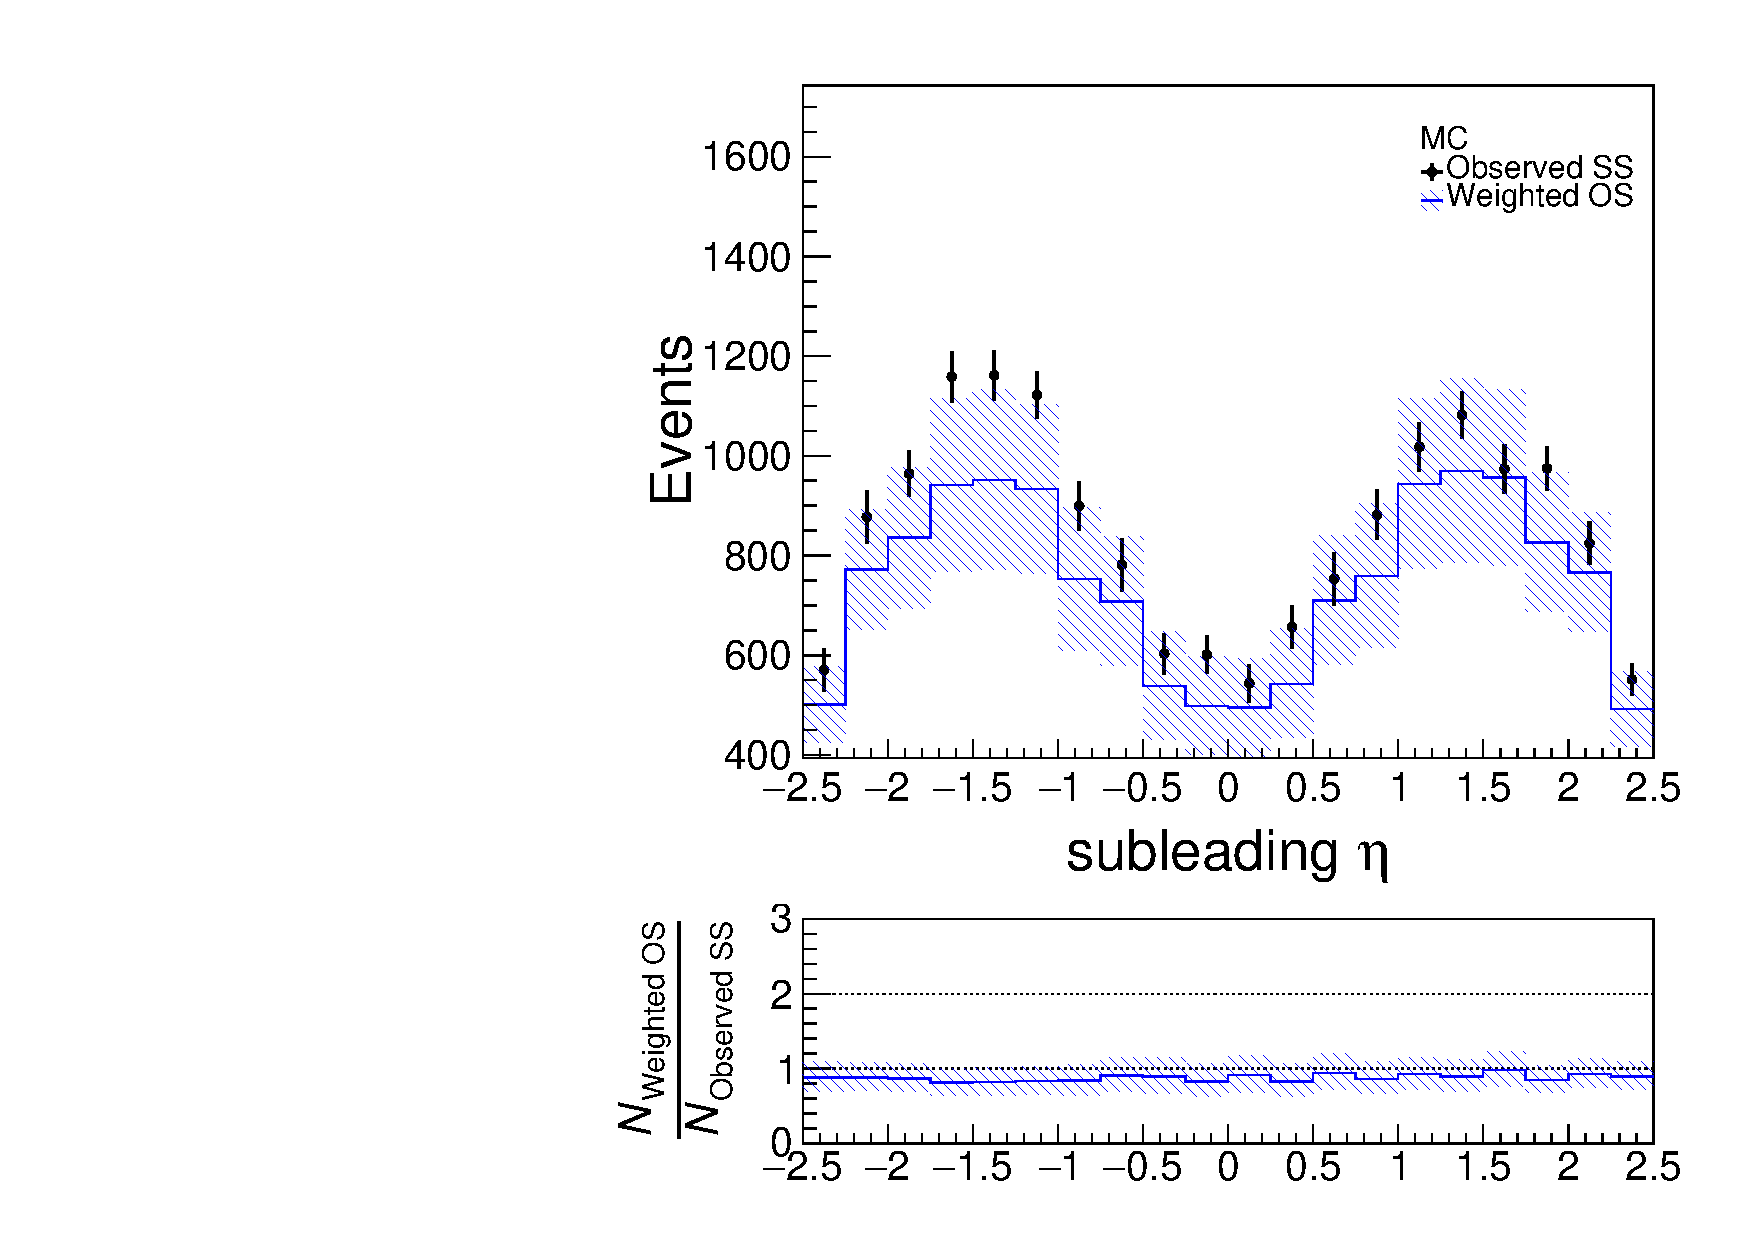
\includegraphics[width=0.3\textwidth]{data/plot/charge_flip/ReweightPlots/plots_NOchfSF/mc_eta_2.pdf}
\caption{The comparison between the weighted OS events and the SS events, with different variables.}
\end{figure}
\end{frame}

\begin{frame}{Likelihood Method : MC Validation Plots}
\begin{figure}
\centering
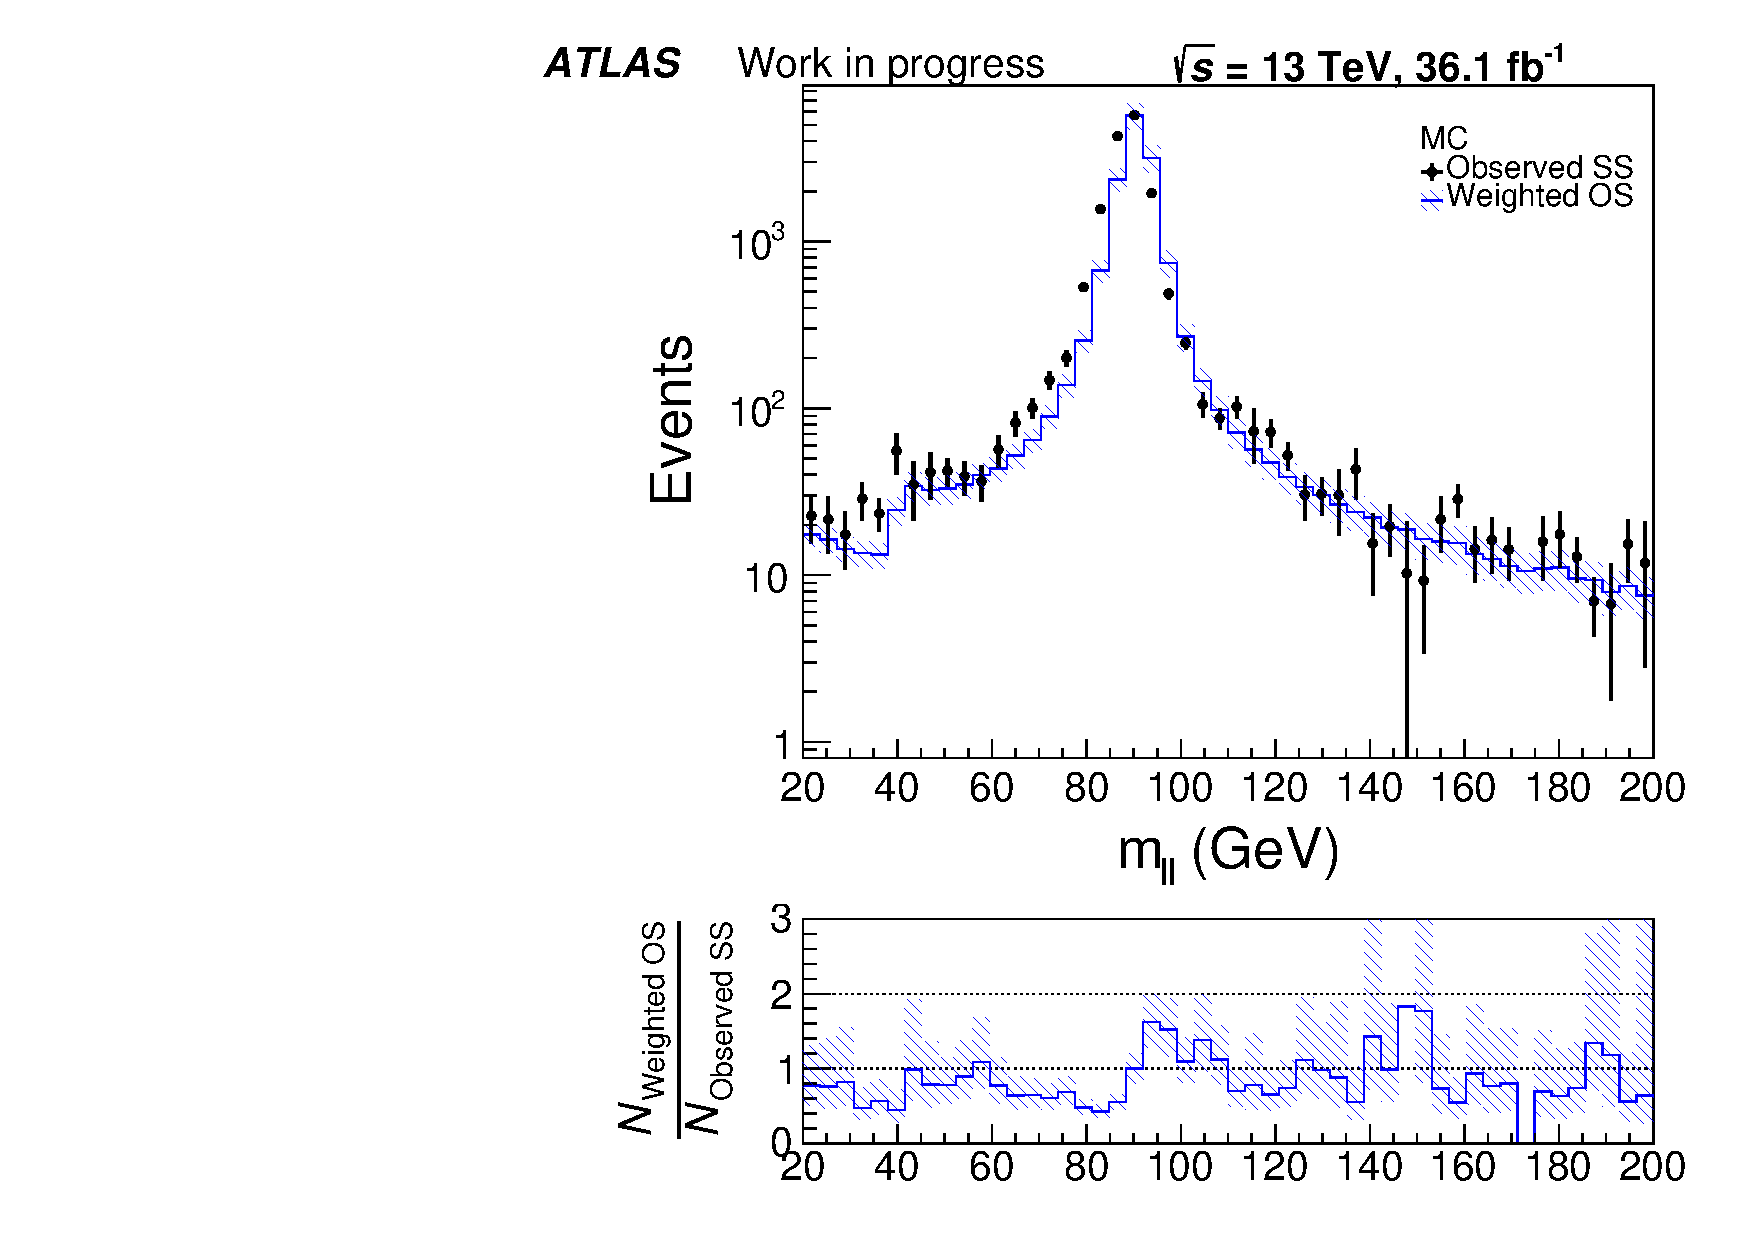
\includegraphics[width=0.3\textwidth]{data/plot/charge_flip/ReweightPlots/plots_NOchfSF/mc_mll.pdf} \\
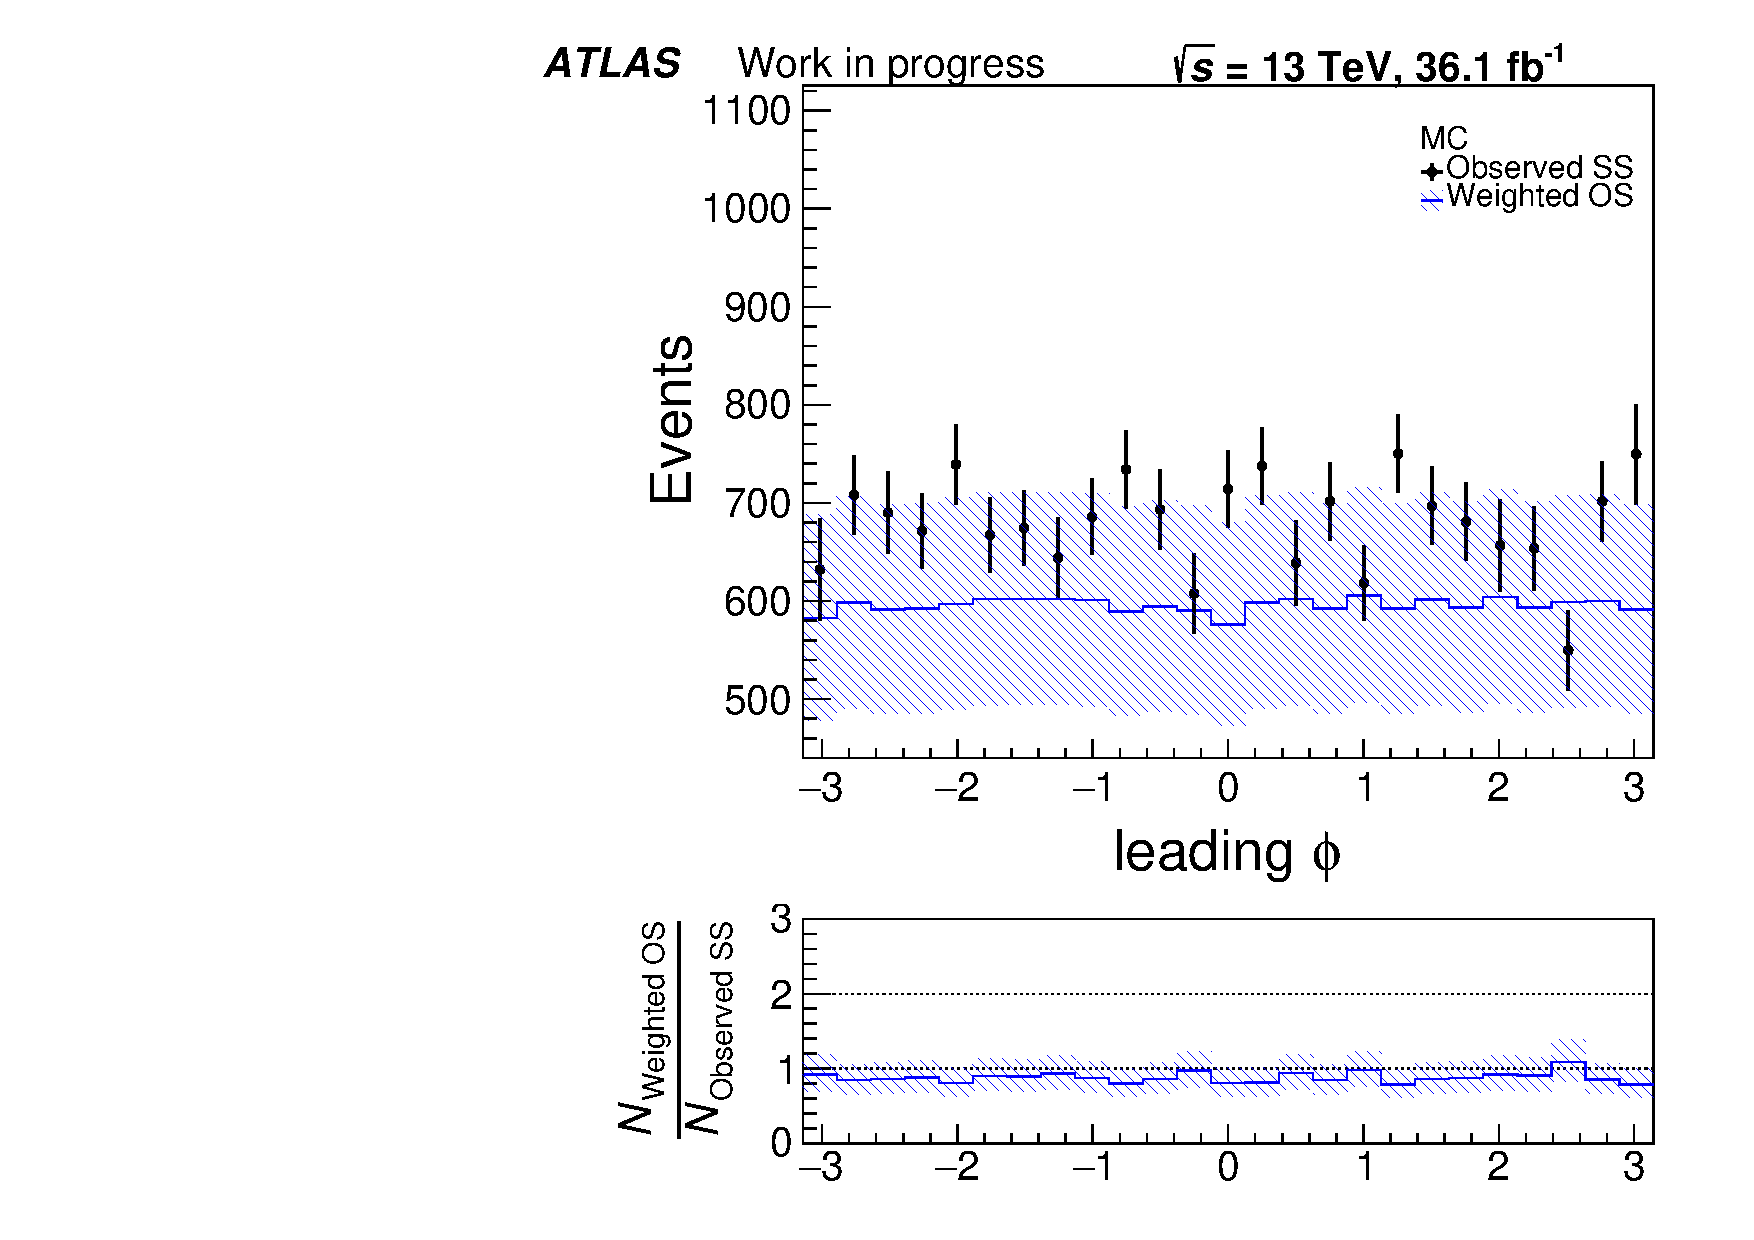
\includegraphics[width=0.3\textwidth]{data/plot/charge_flip/ReweightPlots/plots_NOchfSF/mc_phi_1.pdf}
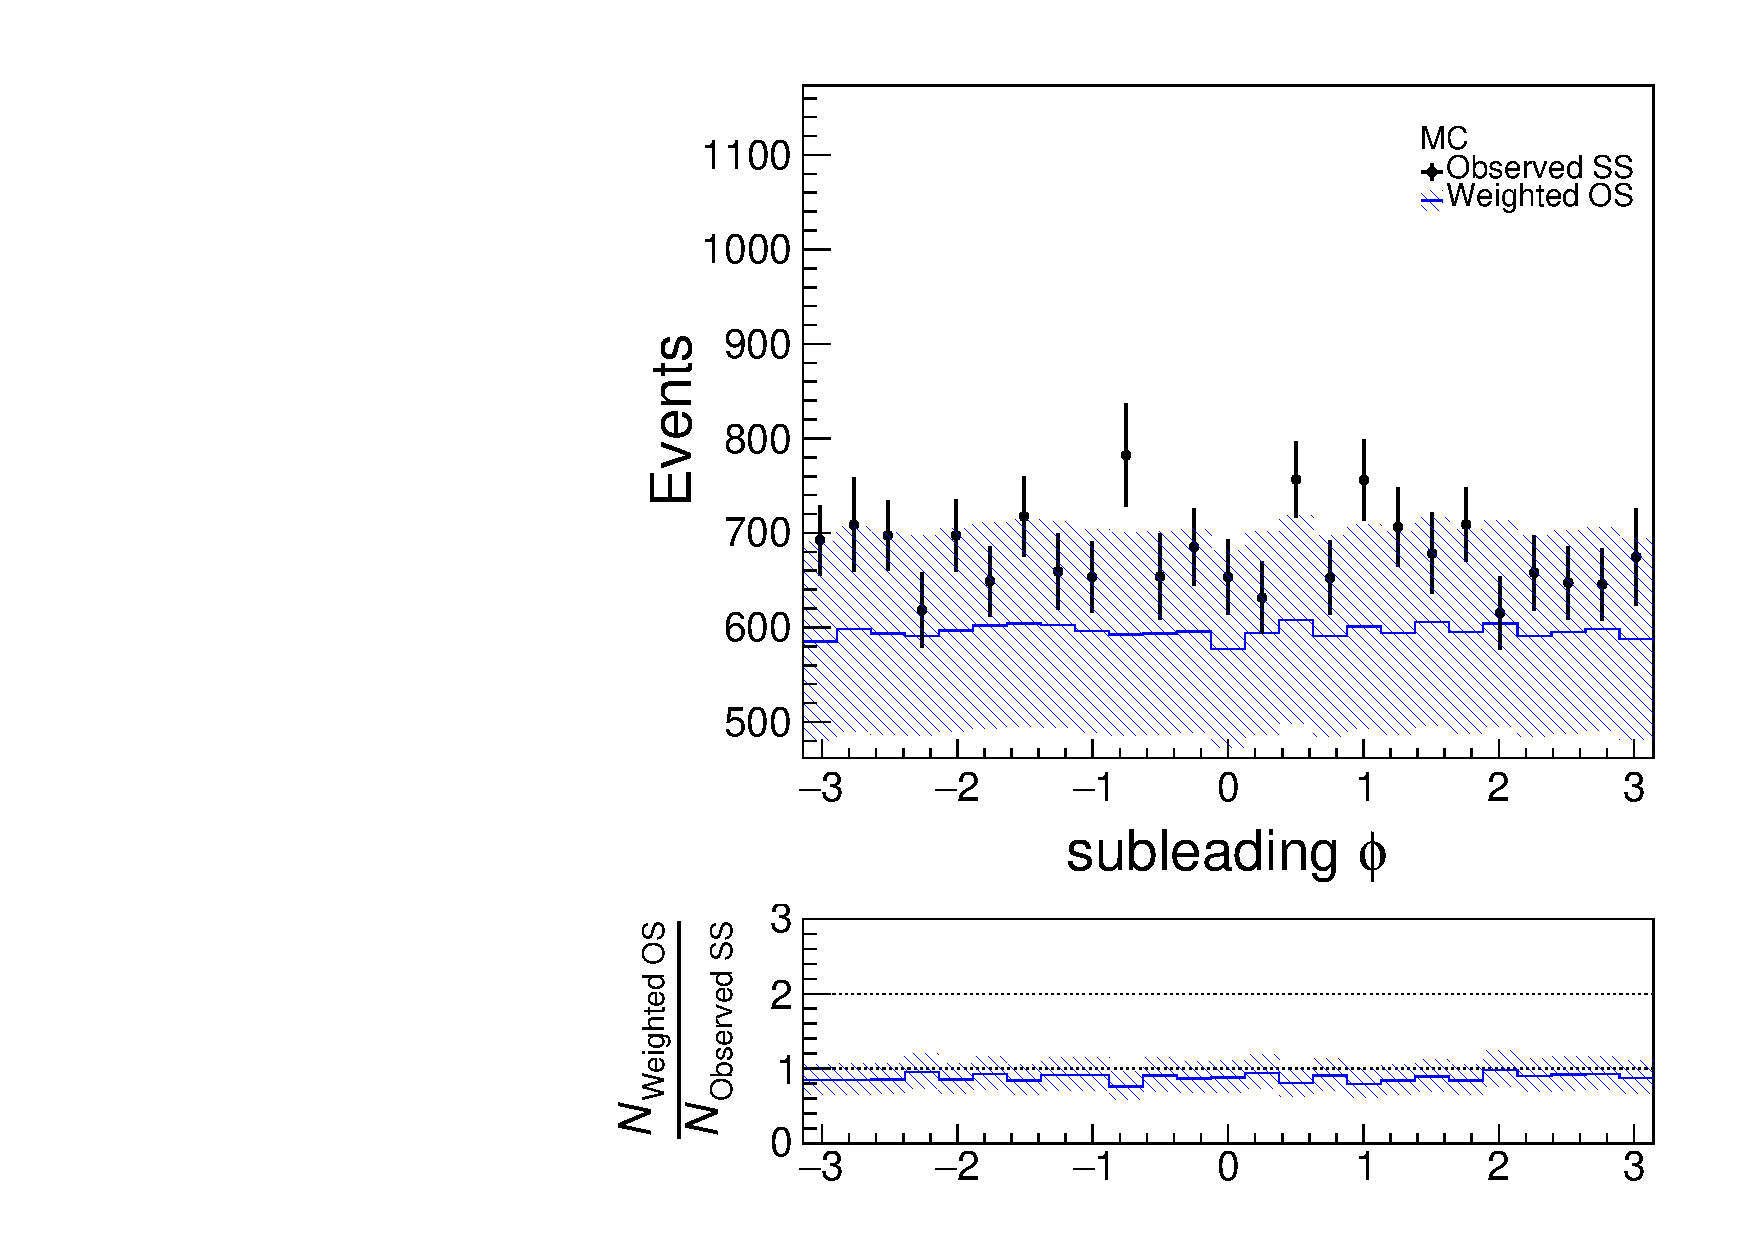
\includegraphics[width=0.3\textwidth]{data/plot/charge_flip/ReweightPlots/plots_NOchfSF/mc_phi_2.pdf}
\caption{The comparison between the weighted OS events and the SS events, with different variables.}
\end{figure}
\end{frame}

\subsection{Fake Lepton Background : Matrix Method}
\begin{frame}
\begin{center}
\huge
Fake Lepton Background : Matrix Method
\end{center}
\end{frame}

\begin{frame}{Fake Lepton Background : Matrix Method}
We can generalize the one-lepton case to the two-leptons case.
\begin{equation*}
\left( \begin{array}{c}
N_{TT} \\
N_{TL} \\
N_{LT} \\
N_{LL}
\end{array} \right)
=
\left( \begin{array}{cccc}
\epsilon_1 \epsilon_2 & \epsilon_1 f_2 & f_1 \epsilon_2 & f_1 f_2 \\
\epsilon_1 \bar{\epsilon_2} & \epsilon_1 \bar{f_2} & f_1 \bar{\epsilon_2} & f_1 \bar{f_2} \\
\bar{\epsilon_1} \epsilon_2 & \bar{\epsilon_1} f_2 & \bar{f_1} \epsilon_2 & \bar{f_1} f_2 \\
\bar{\epsilon_1} \bar{\epsilon_2} & \bar{\epsilon_1} \bar{f_2} & \bar{f_1} \bar{\epsilon_2} & \bar{f_1} \bar{f_2}
\end{array} \right)
\left( \begin{array}{c}
N_{RR} \\
N_{RF} \\
N_{FR} \\
N_{FF}
\end{array} \right)
\end{equation*}
where $\epsilon_1$ is the probability that a leading real lepton passes the signal selection (i.e. tight lepton), $\epsilon_2$ is the probability that a subleading real lepton passes the signal selection (i.e. tight lepton), etc.
\end{frame}

\begin{frame}{Fake Lepton Background : Matrix Method}
We can find $N_{RF}$, $N_{FR}$, $N_{FF}$ by inverting the matrix.

\begin{equation*}
\left( \begin{array}{c}
0 \\
N_{RF} \\
N_{FR} \\
N_{FF}
\end{array} \right)
=
\left( \begin{array}{cccc}
0 & 0 & 0 & 0 \\
0 & 1 & 0 & 0 \\
0 & 0 & 1 & 0 \\
0 & 0 & 0 & 1
\end{array} \right)
\left( \begin{array}{c}
N_{RR} \\
N_{RF} \\
N_{FR} \\
N_{FF}
\end{array} \right)
\end{equation*}

\begin{equation*}
=
\left( \begin{array}{cccc}
0 & 0 & 0 & 0 \\
0 & 1 & 0 & 0 \\
0 & 0 & 1 & 0 \\
0 & 0 & 0 & 1
\end{array} \right)
\left( \begin{array}{cccc}
\epsilon_1 \epsilon_2 & \epsilon_1 f_2 & f_1 \epsilon_2 & f_1 f_2 \\
\epsilon_1 \bar{\epsilon_2} & \epsilon_1 \bar{f_2} & f_1 \bar{\epsilon_2} & f_1 \bar{f_2} \\
\bar{\epsilon_1} \epsilon_2 & \bar{\epsilon_1} f_2 & \bar{f_1} \epsilon_2 & \bar{f_1} f_2 \\
\bar{\epsilon_1} \bar{\epsilon_2} & \bar{\epsilon_1} \bar{f_2} & \bar{f_1} \bar{\epsilon_2} & \bar{f_1} \bar{f_2}
\end{array} \right)^{-1}
\left( \begin{array}{c}
N_{TT} \\
N_{TL} \\
N_{LT} \\
N_{LL}
\end{array} \right)
\end{equation*}
\end{frame}

\begin{frame}{Fake Lepton Background : Matrix Method}
Then, we can find the number of tight-tight leptons due to the fake leptons, $N_{TT}'$

\begin{equation*}
\left( \begin{array}{c}
N_{TT}' \\
N_{TL}' \\
N_{LT}' \\
N_{LL}'
\end{array} \right)
=
\left( \begin{array}{cccc}
\epsilon_1 \epsilon_2 & \epsilon_1 f_2 & f_1 \epsilon_2 & f_1 f_2 \\
\epsilon_1 \bar{\epsilon_2} & \epsilon_1 \bar{f_2} & f_1 \bar{\epsilon_2} & f_1 \bar{f_2} \\
\bar{\epsilon_1} \epsilon_2 & \bar{\epsilon_1} f_2 & \bar{f_1} \epsilon_2 & \bar{f_1} f_2 \\
\bar{\epsilon_1} \bar{\epsilon_2} & \bar{\epsilon_1} \bar{f_2} & \bar{f_1} \bar{\epsilon_2} & \bar{f_1} \bar{f_2}
\end{array} \right)
\left( \begin{array}{c}
0 \\
N_{RF} \\
N_{FR} \\
N_{FF}
\end{array} \right)
\end{equation*}

\begin{equation*}
=
\left( \begin{array}{cccc}
\epsilon_1 \epsilon_2 & \epsilon_1 f_2 & f_1 \epsilon_2 & f_1 f_2 \\
\epsilon_1 \bar{\epsilon_2} & \epsilon_1 \bar{f_2} & f_1 \bar{\epsilon_2} & f_1 \bar{f_2} \\
\bar{\epsilon_1} \epsilon_2 & \bar{\epsilon_1} f_2 & \bar{f_1} \epsilon_2 & \bar{f_1} f_2 \\
\bar{\epsilon_1} \bar{\epsilon_2} & \bar{\epsilon_1} \bar{f_2} & \bar{f_1} \bar{\epsilon_2} & \bar{f_1} \bar{f_2}
\end{array} \right)
\left( \begin{array}{cccc}
0 & 0 & 0 & 0 \\
0 & 1 & 0 & 0 \\
0 & 0 & 1 & 0 \\
0 & 0 & 0 & 1
\end{array} \right)
\end{equation*}

\begin{equation*}
\left( \begin{array}{cccc}
\epsilon_1 \epsilon_2 & \epsilon_1 f_2 & f_1 \epsilon_2 & f_1 f_2 \\
\epsilon_1 \bar{\epsilon_2} & \epsilon_1 \bar{f_2} & f_1 \bar{\epsilon_2} & f_1 \bar{f_2} \\
\bar{\epsilon_1} \epsilon_2 & \bar{\epsilon_1} f_2 & \bar{f_1} \epsilon_2 & \bar{f_1} f_2 \\
\bar{\epsilon_1} \bar{\epsilon_2} & \bar{\epsilon_1} \bar{f_2} & \bar{f_1} \bar{\epsilon_2} & \bar{f_1} \bar{f_2}
\end{array} \right)^{-1}
\left( \begin{array}{c}
N_{TT} \\
N_{TL} \\
N_{LT} \\
N_{LL}
\end{array} \right)
\end{equation*}
\end{frame}

\subsection{Method for measuring real and fake efficiencies}
\begin{frame}
\begin{center}
\huge
Method for measuring real efficiencies
\end{center}
\end{frame}

\begin{frame}{Control Region for Real Efficiencies}
It uses the Z tag-and-probe method to measure the real efficiencies of electrons and muons. \\
Pre-selection:
\begin{itemize}
\item Trigger requirement
\item exactly 2 baseline leptons
\item same flavour and opposite charge ($Z \rightarrow ee$, $Z \rightarrow \mu \mu$)
\item $80 < m_{ll} < 100$
\item $p_T > 20$
\item $|\eta| < 2.47$ for electron, $|\eta| < 2.5$ for muon
\end{itemize}
Requirements for tag lepton
\begin{itemize}
\item $p_T > 25$
\item pass signal requirement
\end{itemize}
\end{frame}

\begin{frame}{Permutation of tag and probe}
Check the probe lepton: \\
Tight lepton: pass signal requirement \\
Loose lepton: pass baseline requirement (include tight lepton) \\
4 possible cases: (slightly simplified)
\begin{itemize}
\item TL: fill loose hist by the subleading lepton
\item LT: fill loose hist by the leading lepton
\item TT: fill both loose and tight hist by the both leading and subleading lepton
\item LL: do nothing
\end{itemize}
The real eff is calculated by
\begin{equation*}
\epsilon = \frac{N_{\text{tight}}}{N_{\text{loose}}}
\end{equation*}
\end{frame}

\begin{frame}{Fake Lepton Background : Results of Real Efficiencies}
The method for measuring the real efficiencies is described in the backup slides.
\begin{figure}
\begin{columns}

\begin{column}{0.5\textwidth}
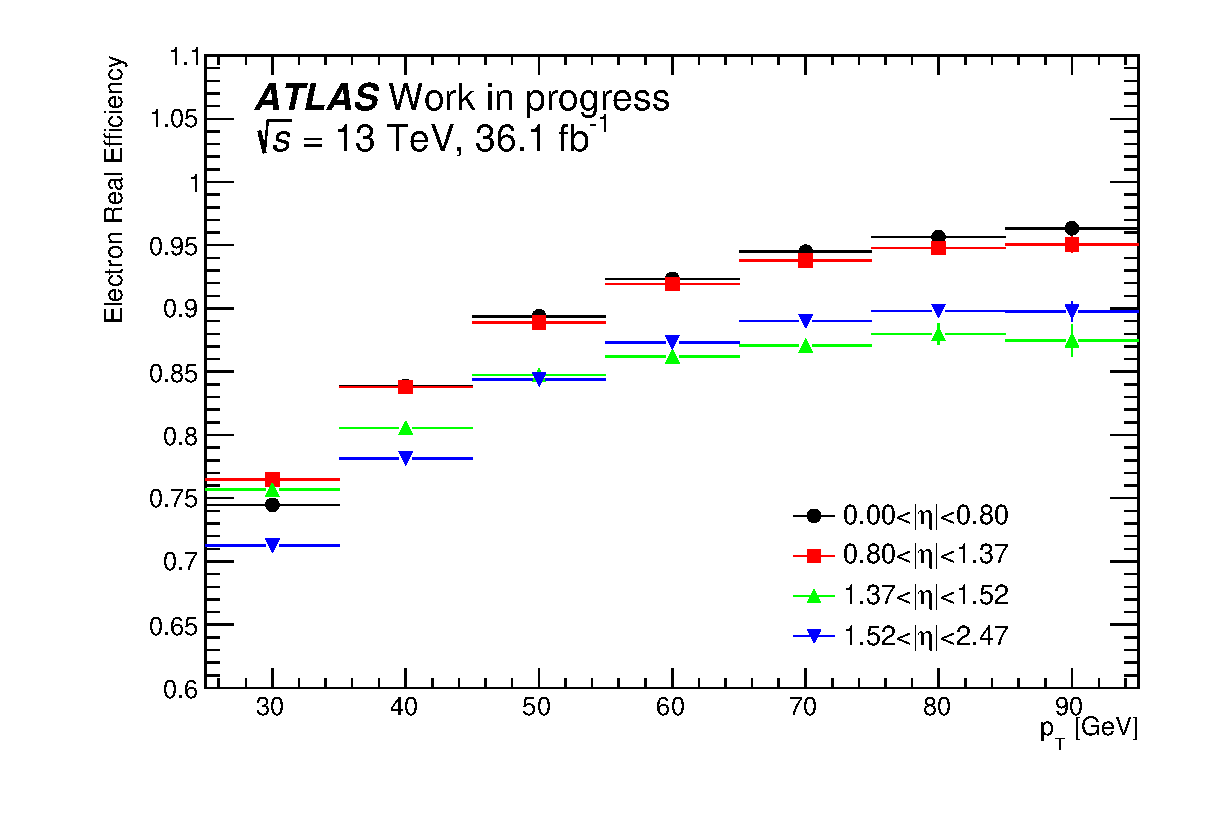
\includegraphics[width=\textwidth]{data/plot/plotRealEffs/El_hEff.eps}
\caption{Electron real efficiency}
\end{column}

\begin{column}{0.5\textwidth}
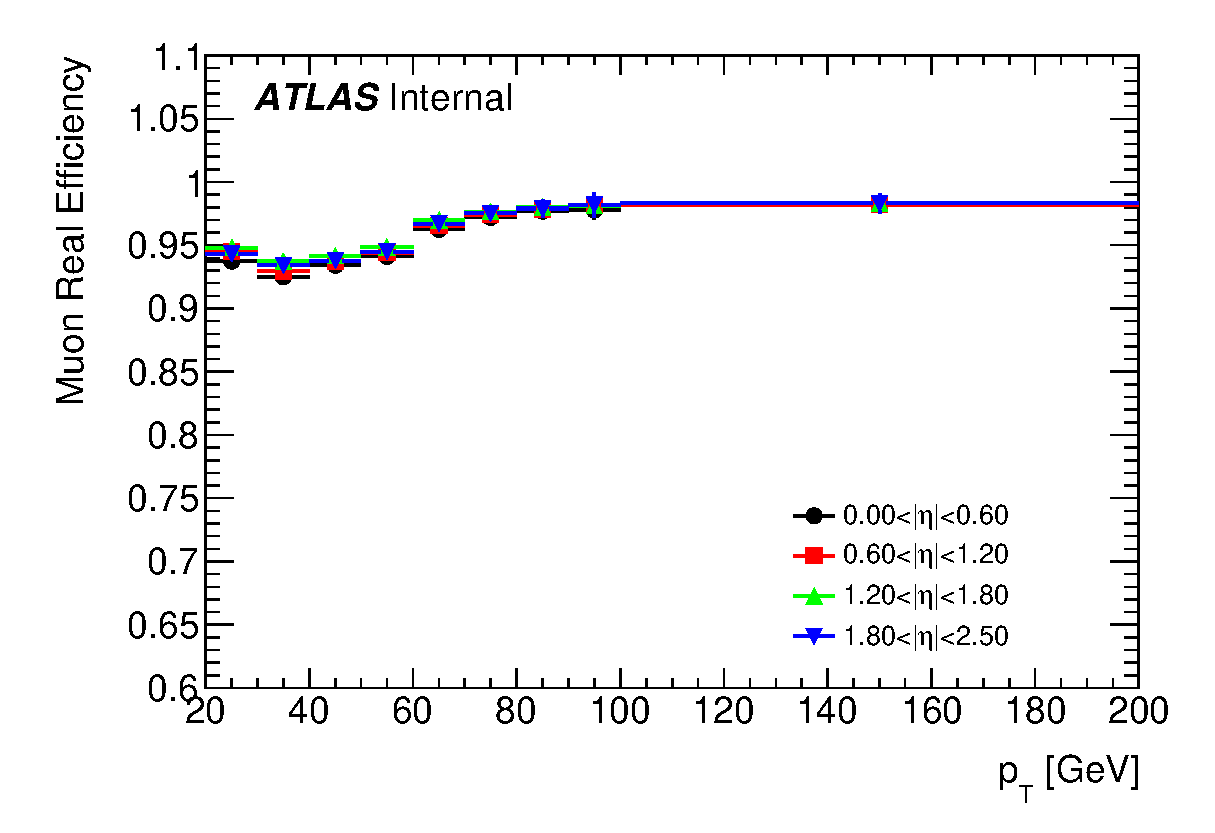
\includegraphics[width=\textwidth]{data/plot/plotRealEffs/Mu_hEff.eps}
\caption{Muon real efficiency}
\end{column}

\end{columns}
\end{figure}
\end{frame}

\begin{frame}
\begin{center}
\huge
Method for measuring fake efficiencies
\end{center}
\end{frame}

\begin{frame}{Control Region for fake eff for muon}
It uses the heavy-flavour fake-enriched region to measure the fake efficiencies of electrons and muons. \\
For muon fake eff, it uses the muon-muon events. \\
Pre-selection for muon-muon events:
\begin{itemize}
\item Trigger requirement
\item exactly 2 baseline muons
\item SS
\item at least 1 jet
\item at least 1 b-jet
\item $p_T > 20$
\item $|\eta| < 2.5$
\end{itemize}
Requirements for the tag lepton
\begin{itemize}
\item $p_T > 40$
\item pass signal requirement
\end{itemize}
\end{frame}

\begin{frame}{Control Region for fake eff for electron}
For electron fake eff, it uses the muon-electron events. \\
Pre-selection for muon-electron events:
\begin{itemize}
\item Trigger requirement
\item exactly 1 baseline electron and 1 baseline muon
\item SS
\item at least 1 jet
\item at least 1 b-jet
\item $p_T > 20$
\item $|\eta| < 2.5$
\end{itemize}
Requirements for the tag lepton
\begin{itemize}
\item muon
\item $p_T > 40$
\item pass signal requirement
\end{itemize}
\end{frame}

\begin{frame}{Calculate the fake eff}
The fake eff is calculated by
\begin{equation*}
\epsilon = \frac{N^{\text{data}}_{\text{tight}} - N^{\text{prompt MC}}_{\text{tight}}}{N^{\text{data}}_{\text{loose}} - N^{\text{prompt MC}}_{\text{loose}}}
\end{equation*}

The prompt lepton is estimated from MC by using the truth information. The prompt lepton is defined by the MCTruthClassifier, with the ParticleType = IsoElectron or IsoMuon.
\end{frame}

\subsection{Validation plots for fake lepton background}
\begin{frame}
\begin{center}
\huge
Validation plots for fake lepton background
\end{center}
\end{frame}

\begin{frame}{ee channel}
\vspace{5mm}
\begin{tabular}{|c|c|c|}
\hline
& Number of events & \\
\hline
Fakes & $860.738787\pm14.359660\pm630.863451$ (9663) & \\
\hline
WZ & $201.069385\pm3.094538$ (39857) & \\
\hline
charge flip & $167.954322\pm1.110819$ (86972) & \\
\hline
WW & $45.176809\pm0.401964$ (21140) & \\
\hline
Rare & $30.757392\pm3.403960$ (1268) & \\
\hline
ZZ & $8.351345\pm0.345416$ (6466) & \\
\hline
$t\bar{t}+V$ & $8.346022\pm0.254296$ (4158) & \\
\hline
Total BG & $1322.394062\pm15.130843\pm630.863451$ (169524) & \\
\hline
Data & $1201$ & \\
\hline

\end{tabular}
\end{frame}

\begin{frame}{ee channel}
\Wider{
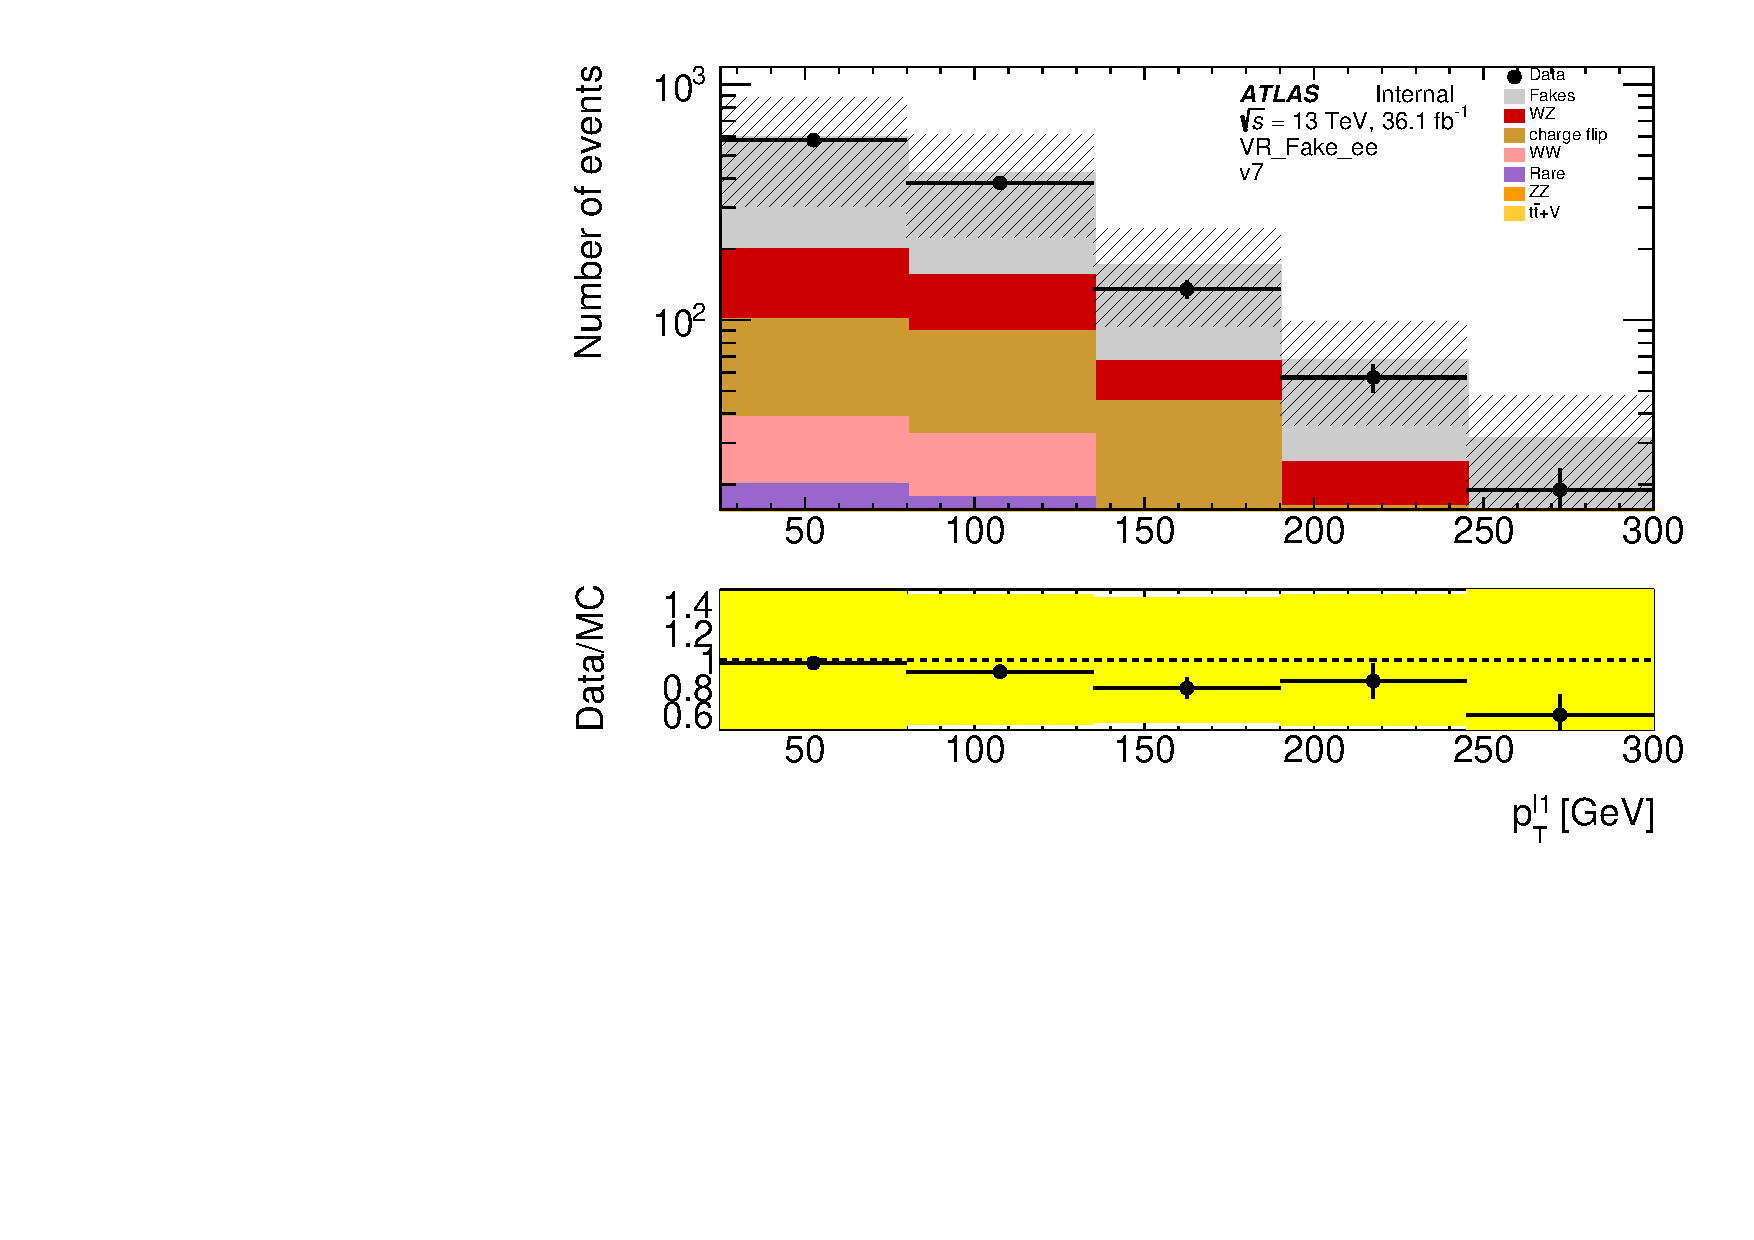
\includegraphics[width=0.4\textwidth]{data/plot/Fake_VR/pt1_VR_Fake_ee}
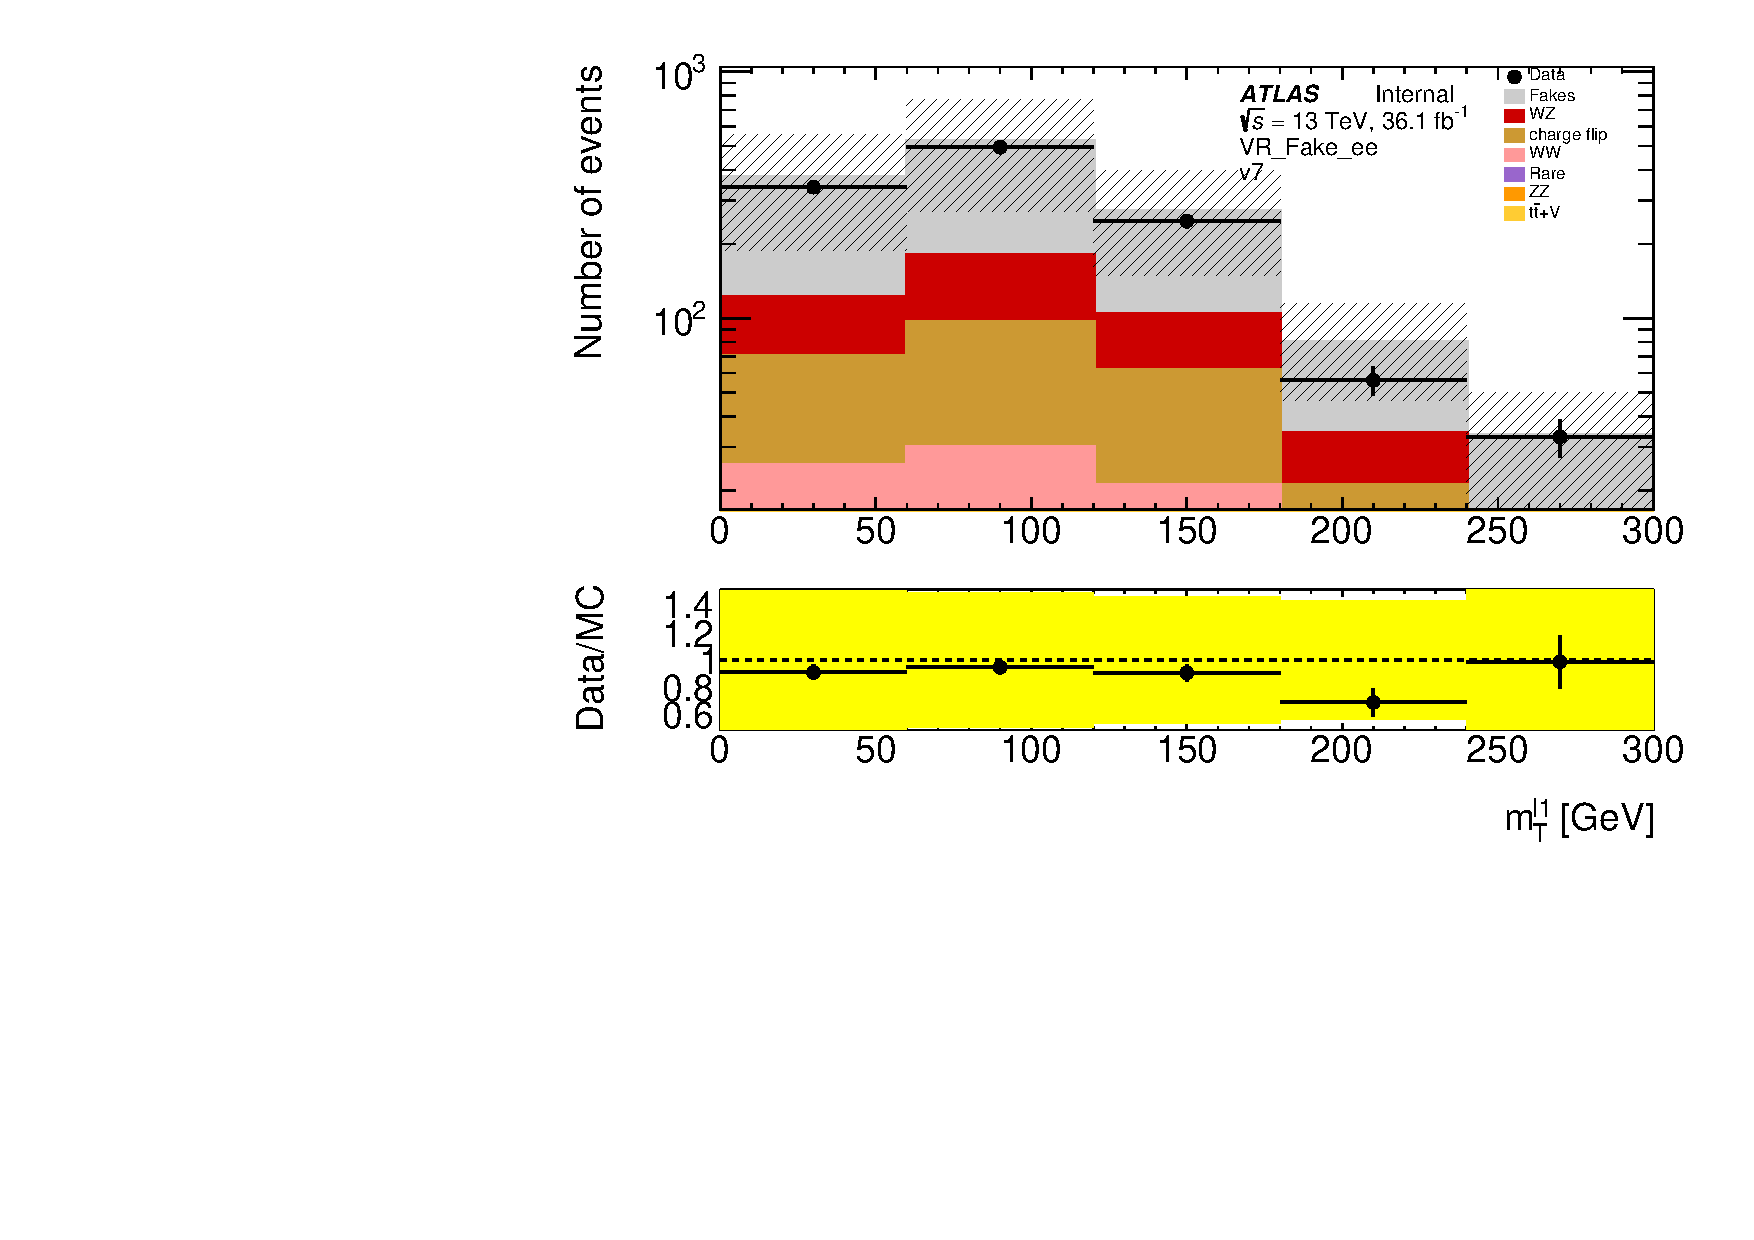
\includegraphics[width=0.4\textwidth]{data/plot/Fake_VR/mt1_VR_Fake_ee} \\
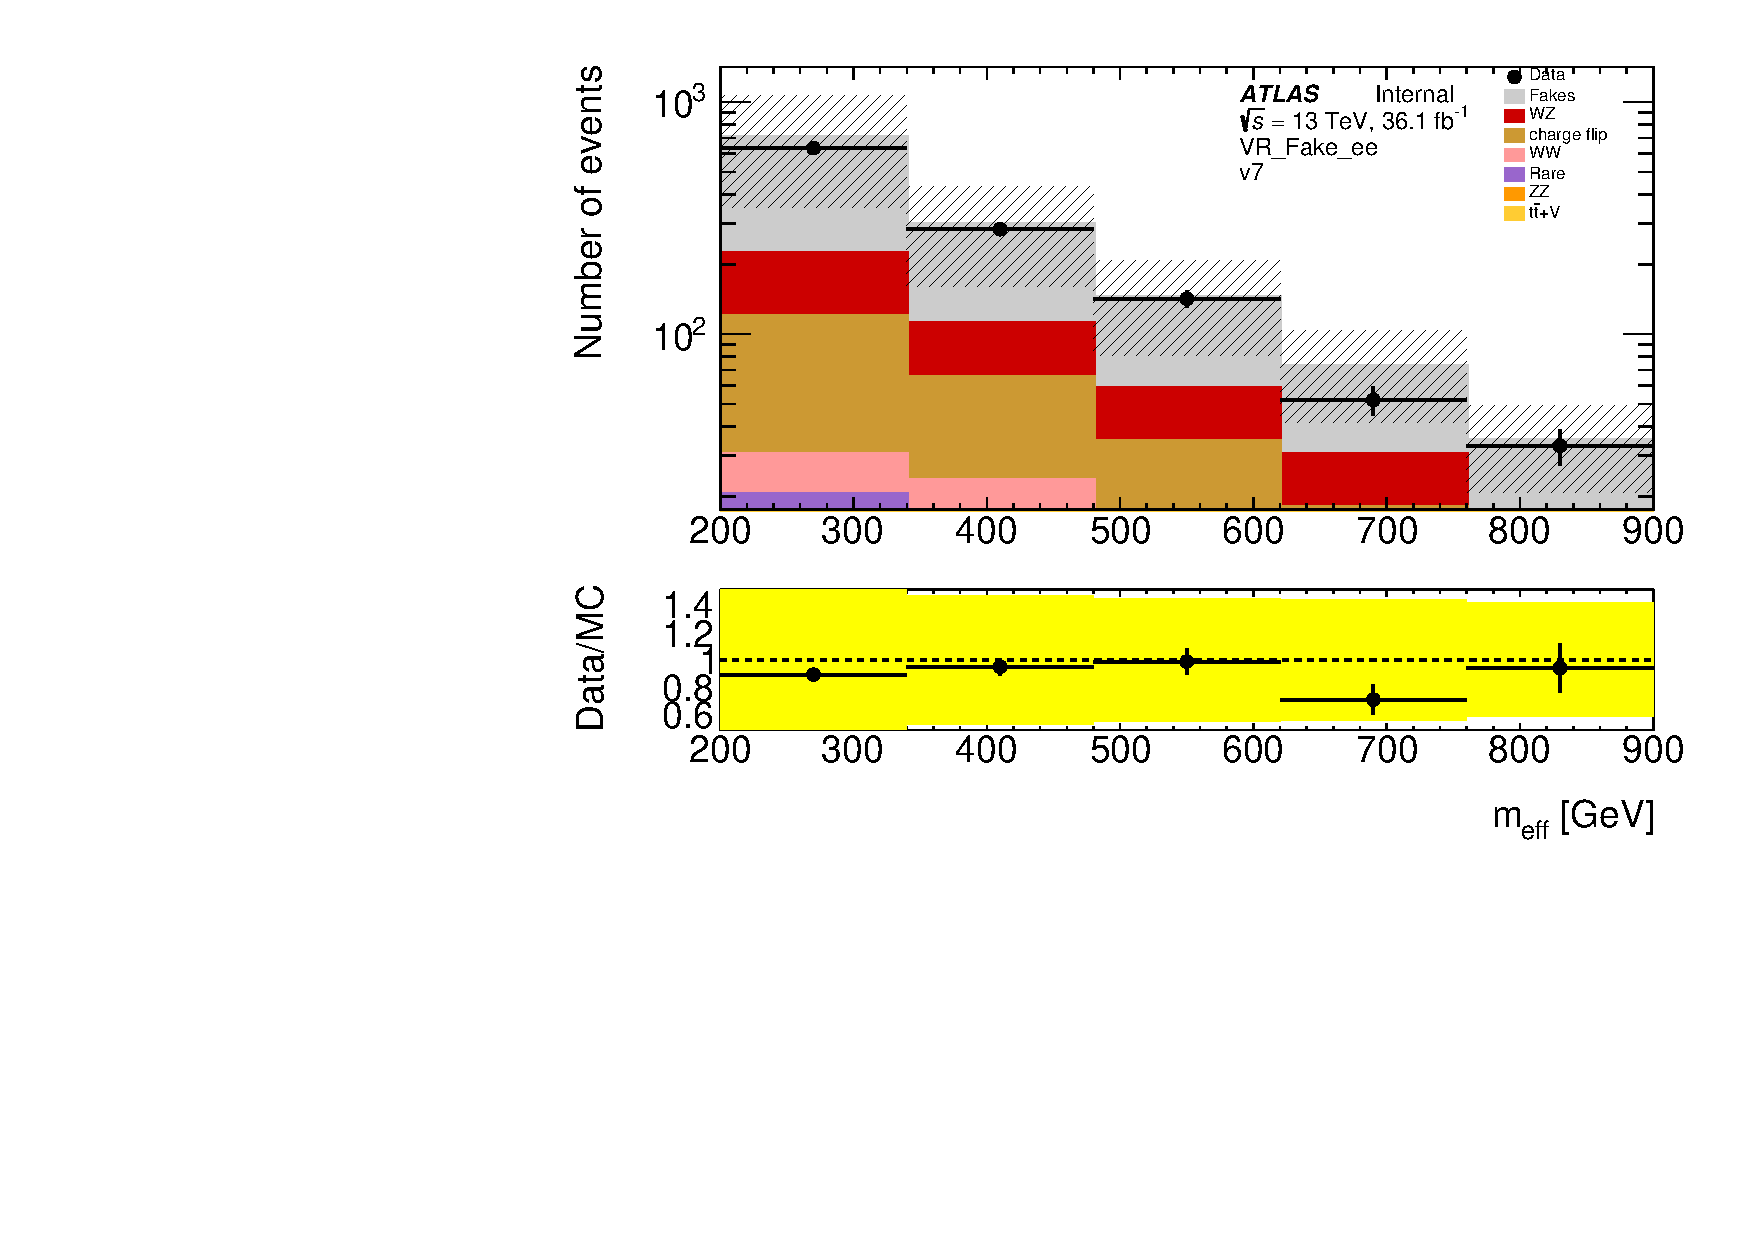
\includegraphics[width=0.4\textwidth]{data/plot/Fake_VR/meff_VR_Fake_ee}
\includegraphics[width=0.4\textwidth]{data/plot/Fake_VR/MET_VR_Fake_ee}
}
\end{frame}

\begin{frame}{mumu channel}
\vspace{5mm}
\begin{tabular}{|c|c|c|}
\hline
& Number of events & \\
\hline
WZ & $209.219829\pm2.994737$ (42458) & \\
\hline
Fakes & $96.203916\pm5.013796\pm70.510979$ (1160) & \\
\hline
WW & $53.675707\pm0.409851$ (25092) & \\
\hline
Rare & $30.460547\pm4.359663$ (1361) & \\
\hline
ZZ & $9.474511\pm0.534342$ (7674) & \\
\hline
$t\bar{t}+V$ & $9.369165\pm0.284944$ (4801) & \\
\hline
charge flip & $0.000000\pm0.000000$ (0) & \\
\hline
Total BG & $408.403674\pm7.324477\pm70.510979$ (82546) & \\
\hline
Data & $454$ & \\
\hline

\end{tabular}
\end{frame}

\begin{frame}{mumu channel}
\Wider{
\includegraphics[width=0.4\textwidth]{data/plot/Fake_VR/pt1_VR_Fake_mumu}
\includegraphics[width=0.4\textwidth]{data/plot/Fake_VR/mt1_VR_Fake_mumu} \\
\includegraphics[width=0.4\textwidth]{data/plot/Fake_VR/meff_VR_Fake_mumu}
\includegraphics[width=0.4\textwidth]{data/plot/Fake_VR/MET_VR_Fake_mumu}
}
\end{frame}

\begin{frame}{emu channel}
\vspace{5mm}
\begin{tabular}{|c|c|c|}
\hline
& Number of events & \\
\hline
Fakes & $702.995427\pm13.784203\pm515.248212$ (8544) & \\
\hline
WZ & $516.828375\pm33.696304$ (94571) & \\
\hline
WW & $110.280002\pm0.578575$ (51615) & \\
\hline
Rare & $58.742111\pm4.005608$ (3037) & \\
\hline
charge flip & $36.901490\pm0.479301$ (36998) & \\
\hline
ZZ & $23.391749\pm0.482387$ (16698) & \\
\hline
$t\bar{t}+V$ & $20.739252\pm0.424107$ (10526) & \\
\hline
Total BG & $1469.878407\pm36.639692\pm515.248212$ (221989) & \\
\hline
Data & $1593$ & \\
\hline

\end{tabular}
\end{frame}

\begin{frame}{emu channel}
\Wider{
\includegraphics[width=0.4\textwidth]{data/plot/Fake_VR/pt1_VR_Fake_emu}
\includegraphics[width=0.4\textwidth]{data/plot/Fake_VR/mt1_VR_Fake_emu} \\
\includegraphics[width=0.4\textwidth]{data/plot/Fake_VR/meff_VR_Fake_emu}
\includegraphics[width=0.4\textwidth]{data/plot/Fake_VR/MET_VR_Fake_emu}
}
\end{frame}

\begin{frame}
\begin{center}
\huge
Pre-selection plots
\end{center}
\end{frame}

\begin{frame}{Yields in pre-selection}
\begin{table}[htbp]
\centering
\tiny

\begin{columns}

\begin{column}{0.5\textwidth}
\scalebox{0.8}{
\begin{tabular}{|c|c|}
\hline
& Number of events \\
\hline
Fakes & $11580.965417\pm45.775452$ (107219) \\
\hline
charge flip & $3622.756937\pm2.810481$ (3375964) \\
\hline
WZ & $691.333566\pm34.238864$ (68626) \\
\hline
ZZ & $66.945860\pm1.049840$ (21749) \\
\hline
Rare & $47.371873\pm4.082859$ (1662) \\
\hline
WW & $38.128141\pm0.388221$ (15666) \\
\hline
$t\bar{t}+V$ & $1.971267\pm0.138488$ (671) \\
\hline
Total BG & $16049.473060\pm57.389305$ (3591557) \\
\hline
(225.0,75.0) & $33.08\pm1.57$ (676) \\
\hline
(187.5,37.5) & $62.09\pm3.13$ (568) \\
\hline
(175.0,0.0) & $74.30\pm3.57$ (556) \\
\hline

\end{tabular}
}
\caption{\tiny Yields in SRjet1}
\end{column}

\begin{column}{0.5\textwidth}
\scalebox{0.8}{
\begin{tabular}{|c|c|}
\hline
& Number of events \\
\hline
Fakes & $6848.284248\pm36.074557$ (66096) \\
\hline
charge flip & $2074.427691\pm2.680118$ (1679673) \\
\hline
WZ & $776.282836\pm5.978666$ (147413) \\
\hline
WW & $153.455294\pm0.679752$ (72175) \\
\hline
Rare & $92.181843\pm6.338615$ (3011) \\
\hline
ZZ & $62.932966\pm1.198123$ (35945) \\
\hline
$t\bar{t}+V$ & $16.375388\pm0.359456$ (6082) \\
\hline
Total BG & $10023.940266\pm37.235816$ (2010395) \\
\hline
(225.0,75.0) & $45.01\pm1.76$ (937) \\
\hline
(187.5,37.5) & $86.02\pm3.84$ (754) \\
\hline
(175.0,0.0) & $107.96\pm5.14$ (743) \\
\hline

\end{tabular}
}
\caption{\tiny Yields in SRjet23}
\end{column}

\end{columns}
\end{table}
\end{frame}

\subsection{pre-selection plots}
\begin{frame}{$p_T^{l1}$}
\Wider{
\includegraphics[width=0.49\textwidth]{pt1_SR_SS_jet1_pre}
\includegraphics[width=0.49\textwidth]{pt1_SR_SS_jet23_pre}
}
\end{frame}

\begin{frame}{$p_T^{l2}$}
\Wider{
\includegraphics[width=0.49\textwidth]{pt2_SR_SS_jet1_pre}
\includegraphics[width=0.49\textwidth]{pt2_SR_SS_jet23_pre}
}
\end{frame}

\begin{frame}{$|\Delta\eta_{ll}|$}
\Wider{
\includegraphics[width=0.49\textwidth]{dEta_SR_SS_jet1_pre}
\includegraphics[width=0.49\textwidth]{dEta_SR_SS_jet23_pre}
}
\end{frame}

\begin{frame}{$E_{\text{T}}^{\text{miss}}$}
\Wider{
\includegraphics[width=0.49\textwidth]{MET_SR_SS_jet1_pre}
\includegraphics[width=0.49\textwidth]{MET_SR_SS_jet23_pre}
}
\end{frame}

\begin{frame}{$m_{\text{eff}}$}
\Wider{
\includegraphics[width=0.49\textwidth]{meff_SR_SS_jet1_pre}
\includegraphics[width=0.49\textwidth]{meff_SR_SS_jet23_pre}
}
\end{frame}

\begin{frame}{$m_{\text{T}}^{l1}$}
\Wider{
\includegraphics[width=0.49\textwidth]{mt1_SR_SS_jet1_pre}
\includegraphics[width=0.49\textwidth]{mt1_SR_SS_jet23_pre}
}
\end{frame}

\begin{frame}{$m_{lj}$/$m_{ljj}$}
\Wider{
\includegraphics[width=0.49\textwidth]{mlj_SR_SS_jet1_pre}
\includegraphics[width=0.49\textwidth]{mlj_SR_SS_jet23_pre}
}
\end{frame}

\begin{frame}{$m_{T2}$}
\Wider{
\includegraphics[width=0.49\textwidth]{mTtwo_SR_SS_jet1_pre}
\includegraphics[width=0.49\textwidth]{mTtwo_SR_SS_jet23_pre}
}
\end{frame}



\begin{frame}
\begin{center}
\huge
N-1 plots
\end{center}
\end{frame}

\begin{frame}{Yields in SR}
\begin{table}[htbp]
\centering
\tiny

\begin{columns}

\begin{column}{0.5\textwidth}
\scalebox{0.8}{
\begin{tabular}{|c|c|c|}
\hline
& Number of events & Significance \\
\hline
Fakes & $3.295434\pm0.819175$ (24) & \\
\hline
WZ & $2.176292\pm0.397871$ (257) & \\
\hline
charge flip & $0.472185\pm0.052737$ (265) & \\
\hline
Rare & $0.443536\pm0.111301$ (56) & \\
\hline
WW & $0.165504\pm0.023455$ (67) & \\
\hline
$t\bar{t}+V$ & $0.124898\pm0.046227$ (36) & \\
\hline
ZZ & $0.055330\pm0.027713$ (31) & \\
\hline
Total BG & $6.733178\pm0.920855$ (736) & \\
\hline
(225.0,75.0) & $3.33\pm0.60$ (60) &$ \bf 0.74$\\
\hline
(187.5,37.5) & $3.77\pm0.95$ (31) &$0.86$\\
\hline
(175.0,0.0) & $4.29\pm0.73$ (36) &$0.98$\\
\hline

\end{tabular}
}
\caption{\tiny Yields in SRjet1}
\end{column}

\begin{column}{0.5\textwidth}
\scalebox{0.8}{
\begin{tabular}{|c|c|c|}
\hline
& Number of events & Significance \\
\hline
WZ & $1.848838\pm0.273025$ (319) & \\
\hline
Fakes & $1.764693\pm0.709215$ (20) & \\
\hline
Rare & $0.731015\pm0.195114$ (48) & \\
\hline
WW & $0.514488\pm0.036878$ (235) & \\
\hline
charge flip & $0.267485\pm0.029086$ (274) & \\
\hline
$t\bar{t}+V$ & $0.141679\pm0.030772$ (67) & \\
\hline
ZZ & $0.067226\pm0.024995$ (24) & \\
\hline
Total BG & $5.335425\pm0.787005$ (987) & \\
\hline
(225.0,75.0) & $2.35\pm0.34$ (58) &$0.57$\\
\hline
(187.5,37.5) & $4.72\pm0.74$ (47) &$\bf 1.26$\\
\hline
(175.0,0.0) & $8.60\pm1.51$ (58) &$2.24$\\
\hline

\end{tabular}
}
\caption{\tiny Yields in SRjet23}
\end{column}

\end{columns}
\end{table}
\end{frame}

\subsection{``N-1'' plots}
\begin{frame}{$p_T^{l1}$}
\Wider{
\includegraphics[width=0.49\textwidth]{pt1_SR_SS_jet1_opt_0}
\includegraphics[width=0.49\textwidth]{pt1_SR_SS_jet23_opt_0}
}
\end{frame}

\begin{frame}{$p_T^{l2}$}
\Wider{
\includegraphics[width=0.49\textwidth]{pt2_SR_SS_jet1_opt_0}
\includegraphics[width=0.49\textwidth]{pt2_SR_SS_jet23_opt_0}
}
\end{frame}

\begin{frame}{$|\Delta\eta_{ll}|$}
\Wider{
\includegraphics[width=0.49\textwidth]{dEta_SR_SS_jet1_opt_0}
\includegraphics[width=0.49\textwidth]{dEta_SR_SS_jet23_opt_0}
}
\end{frame}

\begin{frame}{$E_{\text{T}}^{\text{miss}}$}
\Wider{
\includegraphics[width=0.49\textwidth]{MET_SR_SS_jet1_opt_0}
\includegraphics[width=0.49\textwidth]{MET_SR_SS_jet23_opt_0}
}
\end{frame}

\begin{frame}{$m_{\text{eff}}$}
\Wider{
\includegraphics[width=0.49\textwidth]{meff_SR_SS_jet1_opt_0}
\includegraphics[width=0.49\textwidth]{meff_SR_SS_jet23_opt_0}
}
\end{frame}

\begin{frame}{$m_{\text{T}}^{l1}$}
\Wider{
\includegraphics[width=0.49\textwidth]{mt1_SR_SS_jet1_opt_0}
\includegraphics[width=0.49\textwidth]{mt1_SR_SS_jet23_opt_0}
}
\end{frame}

\begin{frame}{$m_{lj}$/$m_{ljj}$}
\Wider{
\includegraphics[width=0.49\textwidth]{mlj_SR_SS_jet1_opt_0}
\includegraphics[width=0.49\textwidth]{mlj_SR_SS_jet23_opt_0}
}
\end{frame}

\begin{frame}{$m_{T2}$}
\Wider{
\includegraphics[width=0.49\textwidth]{mTtwo_SR_SS_jet1_opt_0}
\includegraphics[width=0.49\textwidth]{mTtwo_SR_SS_jet23_opt_0}
}
\end{frame}



\subsection{Validation Region}
\begin{frame}
\begin{center}
\huge
Validation Region
\end{center}
\end{frame}

\begin{frame}{Validation Region: Check for Signal Contribution}
The signal contribution is below 12\% and 10\% for VRjet1 and VRjet23 respectively.
\begin{figure}
\centering
\includegraphics[width=0.45\textwidth]{data/plot/VR/SignalContamination_VRjet1.eps}
\includegraphics[width=0.45\textwidth]{data/plot/VR/SignalContamination_VRjet23.eps}
\caption{Percentages of signal contribution are shown for the VRjet1 (left) and VRjet23 (right).}
\end{figure}
\end{frame}

\begin{frame}{Validation Region: Check for Background Composition}
The background compositions for VRjet1 and SRjet1 are similar.
\begin{figure}
\centering
\includegraphics[width=0.45\textwidth]{data/plot/VR/BkgComposition_VRjet1.eps}
\includegraphics[width=0.45\textwidth]{data/plot/VR/BkgComposition_SRjet1.eps}
\caption{Background composition for the VRjet1 (left) and SRjet1 (right).}
\end{figure}
\end{frame}

\begin{frame}{Validation Region: Check for Background Composition}
The background compositions for VRjet23 and SRjet23 are similar.
\begin{figure}
\centering
\includegraphics[width=0.45\textwidth]{data/plot/VR/BkgComposition_VRjet23.eps}
\includegraphics[width=0.45\textwidth]{data/plot/VR/BkgComposition_SRjet23.eps}
\caption{Background composition for the VRjet23 (left) and SRjet23 (right).}
\end{figure}
\end{frame}

\begin{frame}{Validation Region : Plots for different variables (VRjet1)}
\Wider{
\includegraphics[width=0.4\textwidth]{data/plot/VR/all_DEtall_VRjet1.eps}
\includegraphics[width=0.4\textwidth]{data/plot/VR/all_Met_VRjet1.eps} \\
\includegraphics[width=0.4\textwidth]{data/plot/VR/all_Meff_VRjet1.eps}
\includegraphics[width=0.4\textwidth]{data/plot/VR/all_Mlj_VRjet1.eps}
}
\end{frame}

\begin{frame}{Validation Region : Plots for different variables (VRjet1)}
\Wider{
\includegraphics[width=0.4\textwidth]{data/plot/VR/all_Mt2_VRjet1.eps}
\includegraphics[width=0.4\textwidth]{data/plot/VR/all_Mt_VRjet1.eps} \\
\includegraphics[width=0.4\textwidth]{data/plot/VR/all_PtLep_VRjet1.eps}
\includegraphics[width=0.4\textwidth]{data/plot/VR/all_PtSublep_VRjet1.eps}
}
\end{frame}

\begin{frame}{Validation Region : Plots for different variables (VRjet1)}
\Wider{
\includegraphics[width=0.4\textwidth]{data/plot/VR/all_Njets_VRjet1.eps}
}
\end{frame}

\begin{frame}{Validation Region : Plots for different variables (VRjet23)}
\Wider{
\includegraphics[width=0.4\textwidth]{data/plot/VR/all_DEtall_VRjet23.eps}
\includegraphics[width=0.4\textwidth]{data/plot/VR/all_Met_VRjet23.eps} \\
\includegraphics[width=0.4\textwidth]{data/plot/VR/all_Meff_VRjet23.eps}
\includegraphics[width=0.4\textwidth]{data/plot/VR/all_Mlj_VRjet23.eps}
}
\end{frame}

\begin{frame}{Validation Region : Plots for different variables (VRjet23)}
\Wider{
\includegraphics[width=0.4\textwidth]{data/plot/VR/all_Mt2_VRjet23.eps}
\includegraphics[width=0.4\textwidth]{data/plot/VR/all_Mt_VRjet23.eps} \\
\includegraphics[width=0.4\textwidth]{data/plot/VR/all_PtLep_VRjet23.eps}
\includegraphics[width=0.4\textwidth]{data/plot/VR/all_PtSublep_VRjet23.eps}
}
\end{frame}

\begin{frame}{Validation Region : Plots for different variables (VRjet23)}
\Wider{
\includegraphics[width=0.4\textwidth]{data/plot/VR/all_Njets_VRjet23.eps}
}
\end{frame}

\end{document}
